\documentclass[12pt,a4paper]{article}
\setlength{\headheight}{13.6pt}
% ============================================================================
% PACKAGES
% ============================================================================
\usepackage[catalan]{babel}
\usepackage[utf8]{inputenc}
\usepackage[T1]{fontenc}
\usepackage{geometry}
\usepackage{graphicx}
\graphicspath{{../}{./}}
\usepackage{float}
\usepackage{subcaption}
\usepackage{amsmath}
\usepackage{amssymb}
\usepackage{booktabs}
\usepackage{multirow}
\usepackage{longtable}
\usepackage{xcolor}
\usepackage{listings}
\usepackage{hyperref}
\usepackage{fancyhdr}
\usepackage{titlesec}
\usepackage{enumitem}
\usepackage{makecell}

% ============================================================================
% CONFIGURACIÓ DE PÀGINA
% ============================================================================
\geometry{
    left=2.5cm,
    right=2.5cm,
    top=3cm,
    bottom=3cm
}

% ============================================================================
% CONFIGURACIÓ D'ESTIL
% ============================================================================
\pagestyle{fancy}
\fancyhf{}
\fancyhead[L]{\small Sistemes d'Informació en les Organitzacions}
\fancyhead[R]{\small Pràctica 1 - 2025/26}
\fancyfoot[C]{\thepage}

\hypersetup{
    colorlinks=true,
    linkcolor=blue,
    citecolor=blue,
    urlcolor=blue
}

% Format de seccions
\titleformat{\section}{\Large\bfseries}{\thesection}{1em}{}
\titleformat{\subsection}{\large\bfseries}{\thesubsection}{1em}{}
\titleformat{\subsubsection}{\normalsize\bfseries}{\thesubsubsection}{1em}{}

% Configuració de codi
\lstset{
    basicstyle=\ttfamily\small,
    breaklines=true,
    frame=single,
    language=Python,
    showstringspaces=false,
    commentstyle=\color{gray},
    keywordstyle=\color{blue},
    stringstyle=\color{red}
}

% ============================================================================
% DOCUMENT
% ============================================================================
\begin{document}

% ============================================================================
% PORTADA
% ============================================================================
\begin{titlepage}
    \centering
    
    % Logo URV
    
\includegraphics[width=0.35\textwidth]{Logo_URV.png}\\[1cm]
    
    {\large Escola Tècnica Superior d'Enginyeria}\\[2cm]
    
    \rule{\linewidth}{0.5mm}\\[0.4cm]
    {\huge\bfseries Pràctica 1}\\[0.3cm]
    {\Large El poder de les dades: Anàlisi d'una cadena\\
    de subministrament simple}\\[0.4cm]
    \rule{\linewidth}{0.5mm}\\[1.8cm]
    
    {\large\textbf{Sistemes d'Informació en les Organitzacions}}\\[0.4cm]
    {\large Curs 2025/2026}\\[2.5cm]
    
    {\large\textbf{Autors:}}\\[0.3cm]
    Nawfal Aissaoui\\
    Salma Jadiani
    
    \vfill
\end{titlepage}


% ============================================================================
% ÍNDEX
% ============================================================================
\tableofcontents
\newpage

% ============================================================================
% 1. INTRODUCCIÓ
% ============================================================================
\section{Introducció}

\subsection{Context i motivació}
% Explicar breument la importància de l'anàlisi de dades en les cadenes de subministrament
% Citar la importància del data science segons l'article de referència
% Contextualitzar el dataset: empreses de comerç electrònic 2015-2018
En l’actualitat, les empreses que treballen amb grans volums de dades tenen una avantatge competitiu clau. Saber analitzar aquesta informació permet prendre decisions més ràpides i precises, especialment en àmbits com la logística i la cadena de subministrament. Aquesta pràctica se centra precisament en això: utilitzar dades reals d’una empresa de comerç electrònic per entendre com funciona la seva activitat entre 2015 i 2018. El dataset inclou informació sobre comandes, clients, productes i enviaments, oferint una visió completa de tot el procés. L’objectiu no és només fer càlculs, sinó entendre com es poden millorar aspectes com els terminis de lliurament, la satisfacció del client o la rendibilitat de cada venda.
\subsection{Objectius de la pràctica}
% Llistar els objectius principals:
% - Comprendre l'estructura del dataset
% - Aplicar tècniques de neteja
% - Realitzar anàlisi descriptiu complet
% - Identificar patrons i correlacions
% - Comunicar resultats efectivament
% - Crear visualitzacions geogràfiques
El nostre propòsit amb aquest treball és doble. D’una banda, vam fer una anàlisi exploratòria de les dades per entendre’n l’estructura, netejar possibles errors i buscar patrons rellevants. Vam preguntar-nos coses com: quins països tenen més risc de retard? Les comandes de quines categories de producte donen més benefici? Hi ha estacions de l’any amb més activitat? D’altra banda, vam voler portar aquesta anàlisi a un nivell visual més intuïtiu, creant mapes interactius que permetessin veure com es distribueixen aquests fenòmens per tot el món. Així, no només treballàvem amb números, sinó que també podíem identificar patrons geogràfics i extreure conclusions espacials.
\subsection{Estructura del document}
% Descripció breu de com s'organitza l'informe
% Secció 2: Descripció del dataset
% Secció 3: Metodologia i eines
% Secció 4: Neteja i preprocessament
% Secció 5: Anàlisi exploratori de dades (Part 1)
% Secció 6: Visualitzacions geogràfiques (Part 2)
% Secció 7: Conclusions
Aquest informe està organitzat per guiar el lector a través de tot el procés que hem seguit. Comencem a la secció 2 presentant el dataset i les variables principals, perquè es pugui entendre sobre què treballem. A la secció 3 expliquem les eines que hem utilitzat, com Python i llibreries específiques per a l’anàlisi i la visualització. La secció 4 descriu com hem netejat i preparat les dades abans de començar l’anàlisi. A la secció 5 entrem de ple en l’anàlisi exploratòria, on mostrem els gràfics, els estadístics i les primeres tendències que hem identificat. La secció 6 està dedicada als mapes interactius, on expliquem com els hem creat i què ens permeten veure. Finalment, a la secció 7 resumim tot el que hem après, comentem les limitacions del treball i proposem idees per a futures millores o aplicacions pràctiques.

\newpage

% ============================================================================
% 2. DESCRIPCIÓ DEL DATASET
% ============================================================================
\section{Descripció del dataset}

\subsection{Característiques generals}
% Dimensions originals: ~180.000 registres
% Període temporal: 2015-2018
% Àmbit geogràfic: internacional
% Taula amb estadístiques bàsiques: nombre de files, columnes, memòria
El dataset \texttt{cadena\_subministrament\_2015\_2018.csv} conté dades reals d'una empresa de comerç electrònic internacional entre 2015 i 2018. Té uns 180.000 registres de comandes de tot el món, amb 58 variables que cobreixen aspectes com clients, productes i logística. Aquesta combinació de volum i diversitat de variables el converteix en una base sòlida per a l'anàlisi exploratòria.

\subsection{Tipologia de variables}
% Crear taula classificant les variables segons tipus:
Per analitzar les dades, hem classificat les variables en sis tipus: categòriques (per descriure), numèriques (per mesurar), binàries (sí/no), temporals (dates), geoespacials (ubicacions) i identificadors (codis únics). Això ens ajuda a triar les eines adequades per a cada anàlisi. La següent taula mostra exemples de cada tipus:




\begin{table}[H]
\centering
\caption{Classificació de les variables del dataset}
\label{tab:tipologia_vars}
\resizebox{\textwidth}{!}{%
\begin{tabular}{lp{12cm}}
\toprule
\textbf{Tipus} & \textbf{Variables principals} \\
\midrule
\textbf{Categòriques} &
\makecell[l]{%
\textit{type}, \textit{delivery\_status}, \textit{category\_name}, \textit{customer\_segment},\\
\textit{market}, \textit{order\_region}, \textit{order\_status}, \textit{shipping\_mode},\\
\textit{product\_name}, \textit{department\_name},\\
\textit{customer\_city}, \textit{customer\_state}, \textit{customer\_country},\\
\textit{order\_city}, \textit{order\_state}, \textit{order\_country},\\
\textit{order\_city\_en}, \textit{order\_state\_en}, \textit{order\_country\_en}
} \\
\midrule
\textbf{Numèriques} &
\makecell[l]{%
\textit{sales}, \textit{sales\_per\_customer}, \textit{benefit\_per\_order},\\
\textit{order\_profit\_per\_order}, \textit{order\_item\_total},\\
\textit{order\_item\_product\_price}, \textit{product\_price},\\
\textit{order\_item\_quantity}, \textit{order\_item\_discount},\\
\textit{order\_item\_discount\_rate}, \textit{order\_item\_profit\_ratio},\\
\textit{days\_for\_shipping\_real}, \textit{days\_for\_shipment\_scheduled}
} \\
\midrule
\textbf{Binàries} &
\makecell[l]{%
\textit{late\_delivery\_risk}, \textit{product\_status}
} \\
\midrule
\textbf{Temporals} &
\makecell[l]{%
\textit{order\_date\_dateorders}, \textit{shipping\_date\_dateorders}
} \\
\midrule
\textbf{Geoespacials} &
\makecell[l]{%
\textit{latitude\_src}, \textit{longitude\_src},\\
\textit{latitude\_dest}, \textit{longitude\_dest},\\
\textit{order\_zipcode}, \textit{customer\_zipcode}, \textit{address\_dest}
} \\
\midrule
\textbf{Identificadors} &
\makecell[l]{%
\textit{order\_id}, \textit{order\_item\_id}, \textit{order\_customer\_id},\\
\textit{customer\_id}, \textit{product\_card\_id},\\
\textit{order\_item\_cardprod\_id}, \textit{category\_id},\\
\textit{product\_category\_id}, \textit{department\_id}
} \\
\bottomrule
\end{tabular}
}
\end{table}

\newpage
% ============================================================================
% 3. METODOLOGIA I EINES
% ============================================================================
\section{Metodologia i eines}

\subsection{Entorn de treball}
% Llenguatge: Python 3.x
% IDE: Jupyter Notebook / VSCode
% Sistema operatiu utilitzat
Com disposem d'un volum elevat de dades (més de 180.000 registres) hem optat per un entorn de programació que ens permetés automatitzar la neteja i generar visualitzacions de qualitat.

Hem desenvolupat tot el codi utilitzant el llenguatge \textit{Python}, treballant principalment sobre \textit{Jupyter Notebooks}. Aquest entorn ens ha permès anar executant el codi per blocs, veure els resultats a l'instant i corregir errors sobre la marxa, cosa que ha agilitzat molt la feina.
\subsection{Llibreries utilitzades}
% Crear taula amb les llibreries i la seva funció
Per dur a terme l'anàlisi i la visualització de les dades, hem fet servir diverses llibreries de Python especialitzades en Data Science. Aquestes eines ens han permès des de la càrrega i neteja del dataset fins a la creació de gràfics i mapes interactius. A continuació es detallen les principals llibreries utilitzades i la seva funció en el projecte:
\begin{table}[H]
\centering
\caption{Eines de Python utilitzades en l’anàlisi}
\label{tab:eines_python}
\resizebox{\textwidth}{!}{%
\begin{tabular}{l p{9.5cm}}
\toprule
\textbf{Llibreria} & \textbf{Ús principal en la pràctica} \\
\midrule
\textbf{pandas} &
Motor principal de l'anàlisi. Càrrega del CSV, neteja de nuls, transformació de dates i càlcul de KPIs agregats. \\
\midrule
\textbf{numpy} &
Suport per a operacions vectorials i càlculs numèrics d'alt rendiment. \\
\midrule
\textbf{matplotlib / seaborn} &
Generació de gràfics estadístics estàtics (histogrames, mapes de calor, diagrames de caixa) per a l'anàlisi exploratòria (EDA). \\
\midrule
\textbf{scikit-learn} &
Implementació d'algorismes de Machine Learning. Utilitzat concretament per al model \textit{K-Means} en la segmentació de clients. \\
\midrule
\textbf{folium} &
Creació de mapes interactius basats en \textit{Leaflet.js}. \\
\midrule
\textbf{geopandas} &
Manipulació de dades geoespacials (GeoJSON) per fusionar les estadístiques de negoci amb les fronteres dels països. \\
\bottomrule
\end{tabular}
}
\end{table}

\newpage  
\newpage
\subsection{Pipeline d'anàlisi}
Per garantir la rigorositat i la reproductibilitat de l'estudi, hem dissenyat i executat un flux de treball seqüencial dividit en 6 fases.

\begin{enumerate}
    \item \textbf{Càrrega i Auditoria Inicial:}
    Vam començar important el dataset cru i realitzant una auditoria tècnica per detectar inconsistències de format, valors nuls i possibles problemes de privacitat (PII).
    
    \item \textbf{Neteja i Preprocessament (Data Wrangling):}
    Execució del sanejament de dades: eliminació de columnes redundants, conversió de formats temporals i creació de variables calculades essencials (\texttt{delay\_days}).
    
    
    \item \textbf{Anàlisi Univariant (Visió General):}
    Estudi de la distribució individual de les variables per detectar asimetries en les vendes i cues de distribució en la rendibilitat.
    
    \item \textbf{Anàlisi Bi/Multivariant (Relacions):}
    Encreuament de variables per buscar patrons causa-efecte (ex: relació entre mode d'enviament i retard).
    
    \item \textbf{Estudis Específics Avançats:}
    Aplicació de tècniques complexes per respondre a problemes estratègics:
    \begin{itemize}
        \item Principi de Pareto (Concentració de catàleg).
        \item Clustering K-Means (Segmentació de clients).
        \item Simulació d'escenaris (Impacte dels descomptes).
    \end{itemize}
    
    \item \textbf{Visualització Geogràfica:}
    Projecció final de les dades sobre mapes interactius per detectar patrons espacials invisibles en els gràfics tradicionals.
\end{enumerate}
\newpage
% ============================================================================
% 4. NETEJA I PREPROCESSAMENT DE DADES
% ============================================================================
\section{Neteja i preprocessament de dades}
Un dels pilars d'aquesta pràctica ha estat assegurar que les dades fossin fiables abans de començar a analitzar-les. No ens hem limitat a executar funcions automàtiques de neteja, sinó que hem realitzat un procés exhaustiu en dues fases per entendre realment què teníem entre mans.
\subsection{Inspecció inicial}
% Estadístiques del dataset original
% Nombre de valors nuls per variable (si n'hi ha)
% Tipus de dades originals
Partíem d'un dataset original amb 180.519 registres i 58 variables. Per abordar aquesta complexitat, vam combinar dues estratègies d'inspecció:

\begin{enumerate}
    \item \textbf{Revisió Semàntica (Manual):} Vam analitzar la definició de cada variable una per una. Això ens va permetre detectar que moltes columnes eren conceptualment idèntiques (ex: IDs vs Noms) o traduccions innecessàries.
    \item \textbf{Revisió Tècnica (Automàtica):} Hem utilitzat Python (Pandas) per detectar errors ``visibles'' per a la màquina: files duplicades exactes, recompte de valors nuls i inconsistències en els tipus de dades (ex: dates que eren text).
\end{enumerate}
\subsection{Variables descartades}
% Explicar per què s'han eliminat certes columnes
% Crear taula justificant cada eliminació:
Fruit d'aquest doble anàlisi, vam decidir eliminar 21 columnes que introduïen soroll o risc. La decisió no va ser aleatòria; cada eliminació està justificada per criteris de redundància, privacitat o qualitat tècnica.

\begin{table}[H]
\centering
\caption{Mostra de variables eliminades i la seva justificació}
\label{tab:vars_eliminades}
\small
\begin{tabular}{lp{9cm}}
\toprule
\textbf{Variable} & \textbf{Motiu d'eliminació} \\
\midrule
category\_id & \textbf{Redundant:} Ja disposem de \textit{category\_name} que és més descriptiu per a l'anàlisi. El mateix aplica a altres IDs. \\
customer\_password & \textbf{Privacitat (PII):} Dada sensible i irrellevant per a l'estudi estadístic. També s'han eliminat \textit{customer\_email} i \textit{customer\_street}. \\
product\_image & \textbf{Format:} És una URL tècnica sense valor analític numèric o categòric. \\
order\_zipcode & \textbf{Qualitat:} Presentava un alt volum de valors nuls difícilment imputables. \\
order\_city\_en & \textbf{Duplicitat:} Traducció innecessària de la variable original \textit{order\_city}. \\
product\_status & \textbf{Constant:} Valor invariable (0) en tot el dataset, per tant no aporta informació (variància zero). \\
\bottomrule
\end{tabular}
\end{table}
\newpage
\subsection{Tractament de valors nuls}
% Si n'hi ha, explicar estratègia seguida:
% - Eliminació de files/columnes
% - Imputació (mitjana, mediana, moda)
% - Creació de categoria ''Unknown''
Després d'eliminar les variables conflictives com \textit{order\_zipcode}, vam tornar a executar un recompte de nuls sobre el dataset resultant. 

El resultat va ser molt satisfactori: les variables restants  estaven completes. Per tant, l'estratègia ha estat l'eliminació preventiva de columnes defectuoses en lloc de la imputació de valors inventats (mitjanes o modes), preservant la veracitat de les dades originals.
\subsection{Tractament d'outliers}
% Identificació d'outliers (mètode IQR, Z-score...)
% Decisió presa: mantenir, eliminar, transformar
% Justificació de la decisió
Durant el cribratge visual (veure secció d'anàlisi exploratòria preliminar), vam detectar valors extrems en variables com \textit{Sales} i \textit{Benefit per Order}.
\begin{itemize}
    \item \textbf{Identificació:} S'observen cues llargues a la distribució (asimetria positiva).
    \item \textbf{Decisió:} Hem decidit mantenir aquests valors. 
    \item \textbf{Justificació:} En el context B2B i Supply Chain, una comanda de valor molt alt o un retard excepcional no són necessàriament errors de dades, sinó situacions reals del negoci que volem analitzar, no amagar.
\end{itemize}
\subsection{Transformacions aplicades}
% Variables derivades creades (si n'hi ha):
% - Diferència entre dates reals i programades
% - Mes/any extret de dates
% - Ratios calculats
% - Categories agrupades
En aquesta fase de neteja, les úniques transformacions han estat de format per garantir la consistència tècnica:
\begin{itemize}
    \item Conversió de \textit{order\_date} i \textit{shipping\_date} a objectes \texttt{datetime} per permetre càlculs temporals posteriors.
    \item Unificació de formats numèrics.
\end{itemize}
La creació de noves variables derivades (com l'extracció del mes o el càlcul de dies de retard) s'ha deixat per a l'etapa d'anàlisi específica per mantenir el dataset base el més net i flexible possible.
\subsection{Dataset final}
% Estadístiques del dataset net
% Dimensions finals
% Afirmació de qualitat de les dades
Un cop completat el procés, disposem d'un conjunt de dades optimitzat i d'alta qualitat per a l'anàlisi.

\begin{itemize}
    \item \textbf{Dimensions finals:} 180.519 registres i 37 columnes.
    \item \textbf{Integritat:} 0 valors nuls en les variables seleccionades.
    \item \textbf{Emmagatzematge:} El resultat s'ha exportat com a \texttt{supply\_chain\_cleaned.csv}.
\end{itemize}

Aquest procés de neteja rigorós ens assegura que les conclusions que extreurem a continuació no estaran esbiaixades per dades brutes o duplicades.
% ============================================================================
% 5. ANÀLISI EXPLORATORI DE DADES (PART 1)
% ============================================================================
\section{Anàlisi exploratori de dades}

% NOTA IMPORTANT: Aquesta és la secció més llarga i valuosa
% Per a CADA estudi, segueix aquesta estructura:
% 5.X.1 Plantejament i hipòtesi
% 5.X.2 Variables i tècniques utilitzades
% 5.X.3 Resultats (gràfics + taules)
% 5.X.4 Interpretació i conclusions
Un cop amb les dades netes, iniciem la fase d'exploració. En lloc de saltar directament a respondre preguntes de negoci, hem aplicat una metodologia de ``dins cap a fora'': primer un cribratge massiu per entendre la forma de les dades i, després, un anàlisi detallat de les relacions clau.

\subsection{Cribratge visual sistemàtic (Screening)}

Abans de començar amb estudis complexos, vam generar de manera automàtica gràfics per a totes les 31 variables del dataset net. Aquest procés, anomenat \textit{cribratge visual} o ``screening'', consisteix en mirar totes les variables d'una tirada per detectar patrons generals, anomalies o problemes evidents abans de fer anàlisis més profunds. És com fer una primera fotografia de les dades per saber per on començar.

Vam classificar les variables en tres grups i generar els gràfics adequats per a cadascuna, segons es resumeix a la Taula~\ref{tab:cribratge_summary}:

\begin{table}[H]
\centering
\caption{Resum del procés de cribratge visual}
\label{tab:cribratge_summary}
\small
\begin{tabular}{lccp{8cm}}
\toprule
\textbf{Tipus de variable} & \textbf{Quantitat} & \textbf{Gràfic utilitzat} & \textbf{Propòsit} \\
\midrule
Categòriques & 16 & Barres (Top 20) & Identificar categories dominants i concentracions extremes. \\
Numèriques & 14 & Histograma + KDE & Veure forma de la distribució, asimetries i outliers. \\
Binàries & 1 & Barres + Sectors & Entendre la proporció entre les dues categories (ex: retard sí/no). \\
\bottomrule
\end{tabular}
\end{table}

El resultat complet d'aquest cribratge (31 gràfics) es pot trobar a la carpeta \texttt{figures/exploratory/} del codi adjunt. A continuació mostrem alguns exemples representatius que van permetre extreure les primeres observacions generals.

\subsubsection{Exemples visuals del cribratge}

% EXEMPLE 1: Concentració extrema
\begin{figure}[H]
\centering
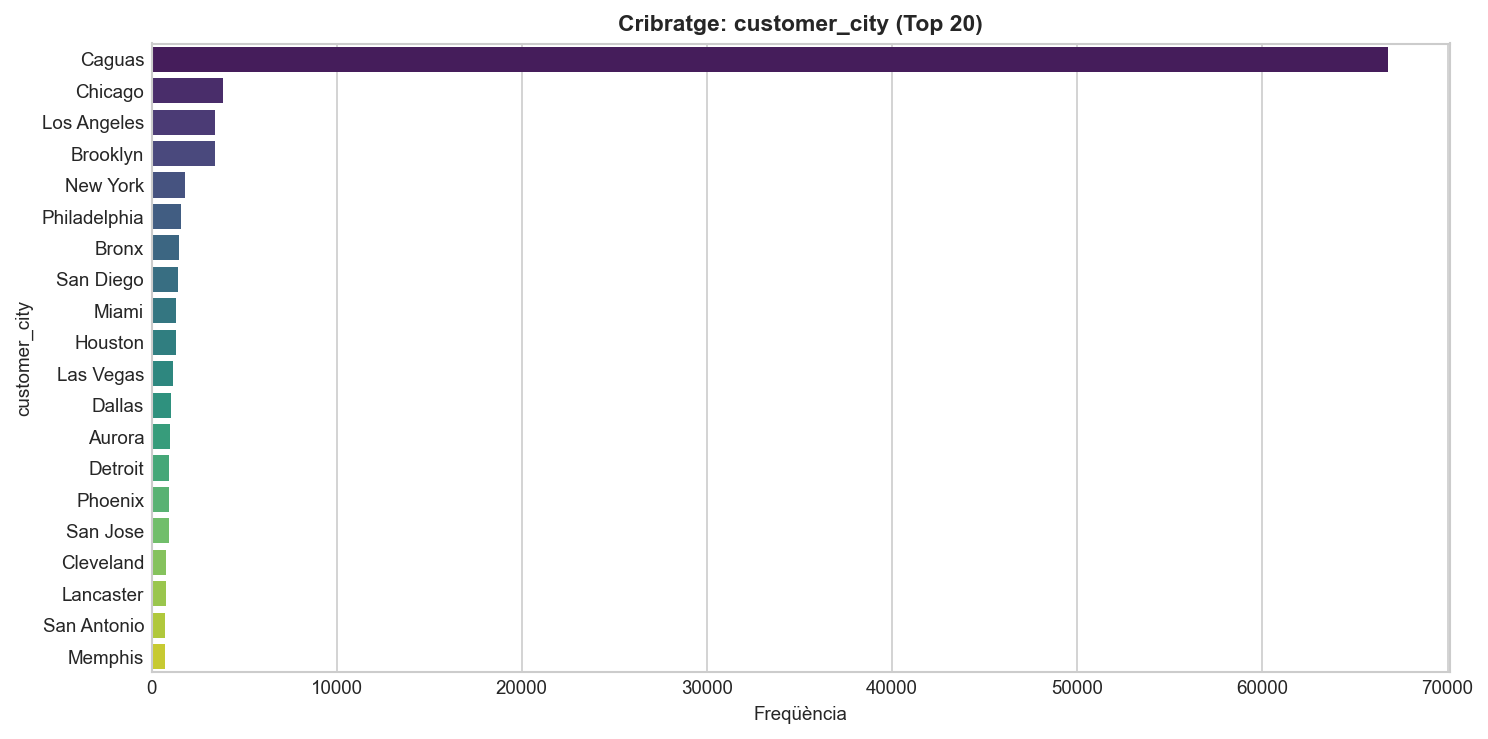
\includegraphics[width=0.8\textwidth]{figures/exploratory/cat_customer_city.png}
\caption{Cribratge de \texttt{customer\_city}: concentració extrema a Caguas (Puerto Rico).}
\label{fig:crib_customer_city}
\end{figure}

La Figura~\ref{fig:crib_customer_city} il·lustra una de les anomalies més evidents: mentre la majoria de ciutats tenen pocs centenars de comandes, \textbf{Caguas} acumula més de 65.000 registres. Això indica una dependència geogràfica molt forta que podria afectar l'estratègia logística.

% EXEMPLE 2: Distribució de retards
\begin{figure}[H]
\centering
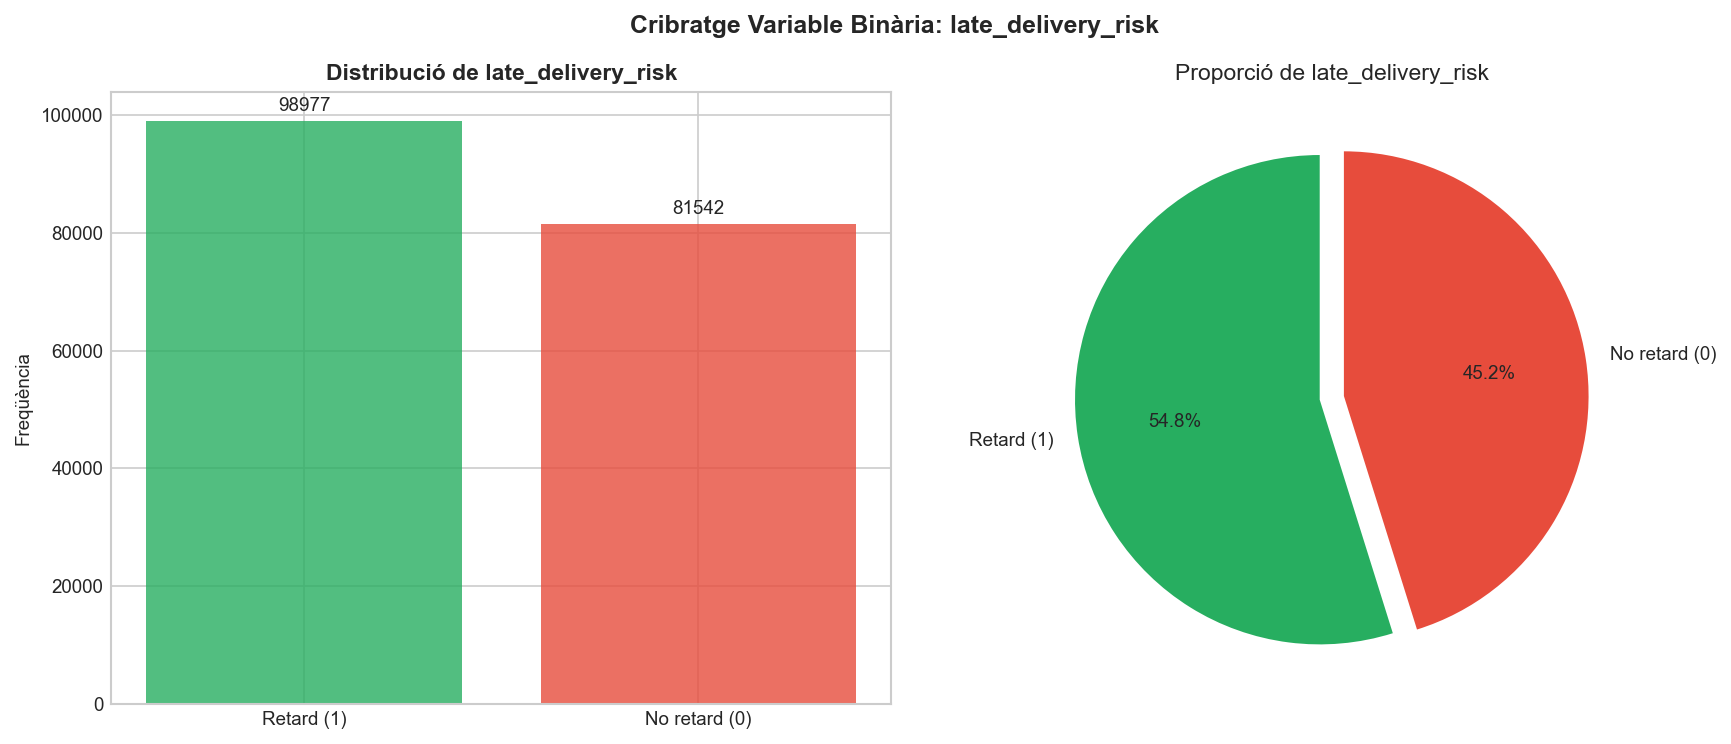
\includegraphics[width=0.8\textwidth]{figures/exploratory/bin_late_delivery_risk.png}
\caption{Cribratge de \texttt{late\_delivery\_risk}: més de la meitat de les comandes tenen risc de retard.}
\label{fig:crib_late_delivery}
\end{figure}

La Figura~\ref{fig:crib_late_delivery} confirma un problema operatiu greu: el \textbf{54.8\%} de les comandes presenten risc de retard. Aquesta dada justifica que una part important de l'anàlisi posterior se centri en la logística i els terminis de lliurament.

% EXEMPLE 3: Distribució de vendes
\begin{figure}[H]
\centering
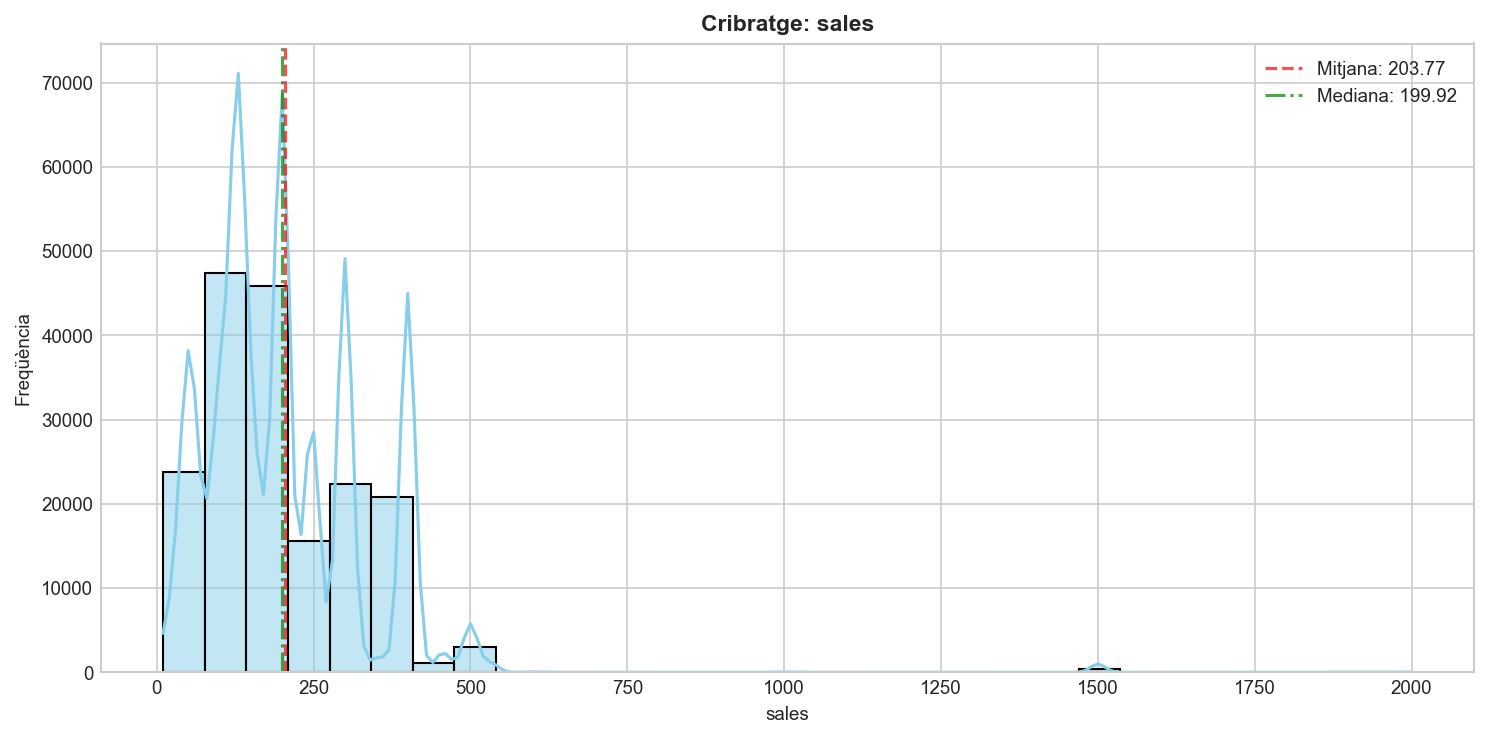
\includegraphics[width=0.8\textwidth]{figures/exploratory/num_sales.png}
\caption{Cribratge de \texttt{sales}: distribució asimètrica amb cua llarga cap a la dreta.}
\label{fig:crib_sales}
\end{figure}

La Figura~\ref{fig:crib_sales} mostra com la variable de vendes té una \textbf{distribució asimètrica}: la majoria de comandes són de valor baix (menys de 500\texteuro),amb presència de valors extrems aïllats (cap a 1.500). Això ens alerta que la mitjana podria no ser representativa.

\subsubsection{Insights principals del cribratge}

A partir de la revisió sistemàtica de tots els gràfics, vam identificar els patrons més rellevants:

\begin{itemize}
    \item \textbf{Distribucions asimètriques (Cues llargues):} Variables com \textit{Sales} o \textit{Order Item Quantity} no segueixen una distribució normal. La majoria de comandes són d'imports petits, però hi ha una ``cua'' de comandes molt grans que estiren la mitjana cap amunt. Això indica que la mitjana pot no ser el millor representant.
    \item \textbf{Normalitat en els beneficis:} Curiosament, la variable \textit{Benefit per Order} presenta una distribució semblant a una campana de Gauss (normal), centrada lleugerament en positiu, però amb una quantitat rellevant de valors negatius (pèrdues) que caldrà investigar.
    
    \item \textbf{Concentració extrema en categories:} A més del cas de Caguas, variables com \textit{Category Name} o \textit{Department Name} mostren que el volum de negoci es concentra en poques categories (Cleats, Men's Footwear, Fan Shop).
    
    \item \textbf{Problema crític de retards:} Confirmat tant per la variable binària com per \textit{delivery\_status}, on ``Late delivery'' és l'estat més freqüent.
    
    \item \textbf{Preus i descomptes estandarditzats:} Els histogrames de \textit{Product Price} i \textit{Order Item Discount Rate} mostren pics clars a valors concrets, indicant que l'empresa treballa amb preus fixos i descomptes per graons, amb una freqüència d'aparició pràcticament idèntica per a tots els nivells.
\end{itemize}

Gràcies a aquest cribratge, vam poder seleccionar les variables que realment aportaven informació (les que tenien variància i patrons clars) i descartar les que, tot i ser tècnicament correctes, no mostraven comportaments rellevants per al negoci. A més, vam definir les preguntes d'investigació que abordarem a la següent fase: l'anàlisi exploratòria detallada.
\subsection{Anàlisi univariant}
Un cop filtrades les dades, hem estudiat les variables una per una per entendre el comportament base del negoci. Aquesta fase és crítica per detectar anomalies que podrien distorsionar els models posteriors. Donat l'elevat nombre de variables disponibles, hem aplicat un criteri de priorització basat en l'impacte estratègic:

\begin{itemize}
    \item \textbf{Crítiques:} Variables que afecten directament la satisfacció del client o la rendibilitat.
    \item \textbf{Alt:} Variables amb gran influència en les operacions.
    \item \textbf{Mitjanes/Derivades:} Variables suport o calculades.
\end{itemize}

Ens hem centrat principalment en aquelles variables que actuen com a indicadors clau de rendiment (KPIs) o que presenten anomalies estadístiques rellevants:
\begin{enumerate}
    \item \textbf{Variables de Servei:} \texttt{delivery\_status} i \texttt{delay\_days}, ja que la puntualitat és crítica per a la retenció de clients.
    \item \textbf{Variables Financeres:} \texttt{sales} i \texttt{benefit\_per\_order}, per entendre l'estructura d'ingressos i detectar focus de pèrdues.
\end{enumerate}

La resta de variables s'analitzen en funció de la seva prioritat i només es presenten aquelles que mostren comportaments rellevants per al negoci.
\subsubsection{Anàlisi de variables Categòriques: La crisi dels retards}
L'anàlisi de freqüències ha revelat immediatament el problema operatiu més greu de l'empresa. Com es pot veure a la Figura \ref{fig:delivery_status}, la puntualitat és l'assignatura pendent.

\begin{figure}[H]
    \centering
    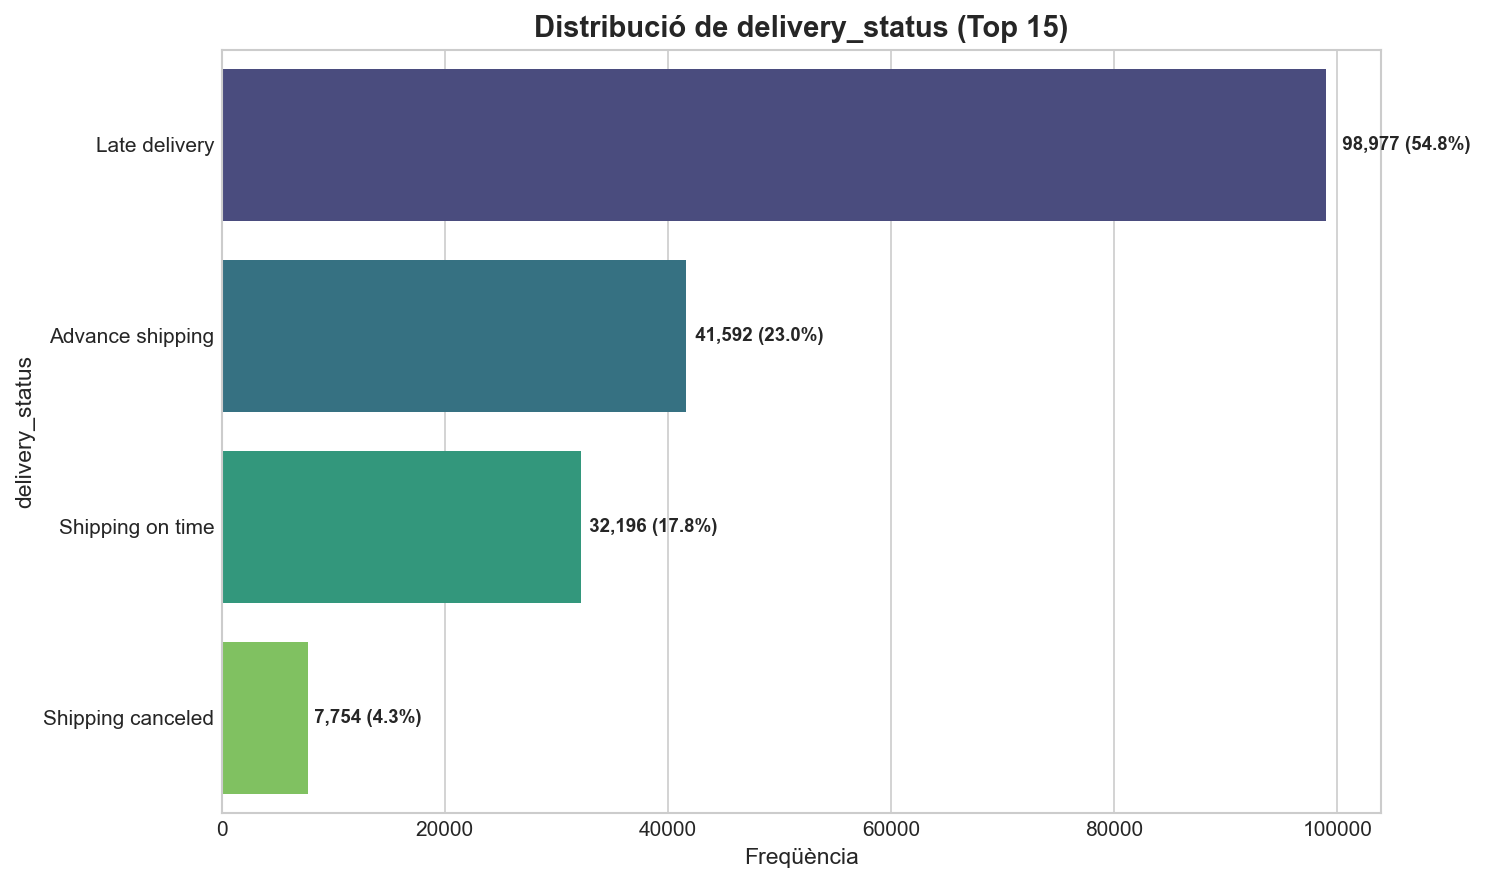
\includegraphics[width=0.85\textwidth]{figures/final/01_univariant/categoriques/cat_delivery_status.png}
    \caption{Distribució de l'estat dels lliuraments. El color dominant mostra una majoria de retards.}
    \label{fig:delivery_status}
\end{figure}

Les dades són contundents: un \textbf{54.8\% dels enviaments arriben tard} (\textit{Late delivery}). Això significa que més de la meitat dels clients no reben el producte quan se'ls va prometre. Només un 23\% aproximadament arriba ''A temps'', mentre que els enviaments avançats representen una quota similar. Afortunadament, la taxa de cancel·lacions és baixa, però el risc de retard és molt alt.

Pel que fa al perfil de l'activitat, hem identificat que:
\begin{itemize}
    \item \textbf{Mercat principal:} L'activitat es concentra a \textbf{LATAM (28.6\%)}, seguit de prop per Europa, Asia Pacífica i USCA.
    \item \textbf{Tipus de client:} El segment \textit{Consumer} (particulars) representa el 51.8\% de les comandes, superant al \textit{Corporate}.
    \item \textbf{Logística:} El mode d'enviament estàndard és el preferit pel 59.7\% dels clients.
\end{itemize}

\subsubsection{Anàlisi de variables Numèriques: Rendibilitat i Vendes}
En passar a les variables quantitatives, hem detectat patrons financers complexos que requereixen atenció.

\paragraph{Distribució de les Vendes}
La variable \texttt{sales} mostra una clara asimetria positiva (Skewness: 2.88).

\begin{figure}[H]
    \centering
    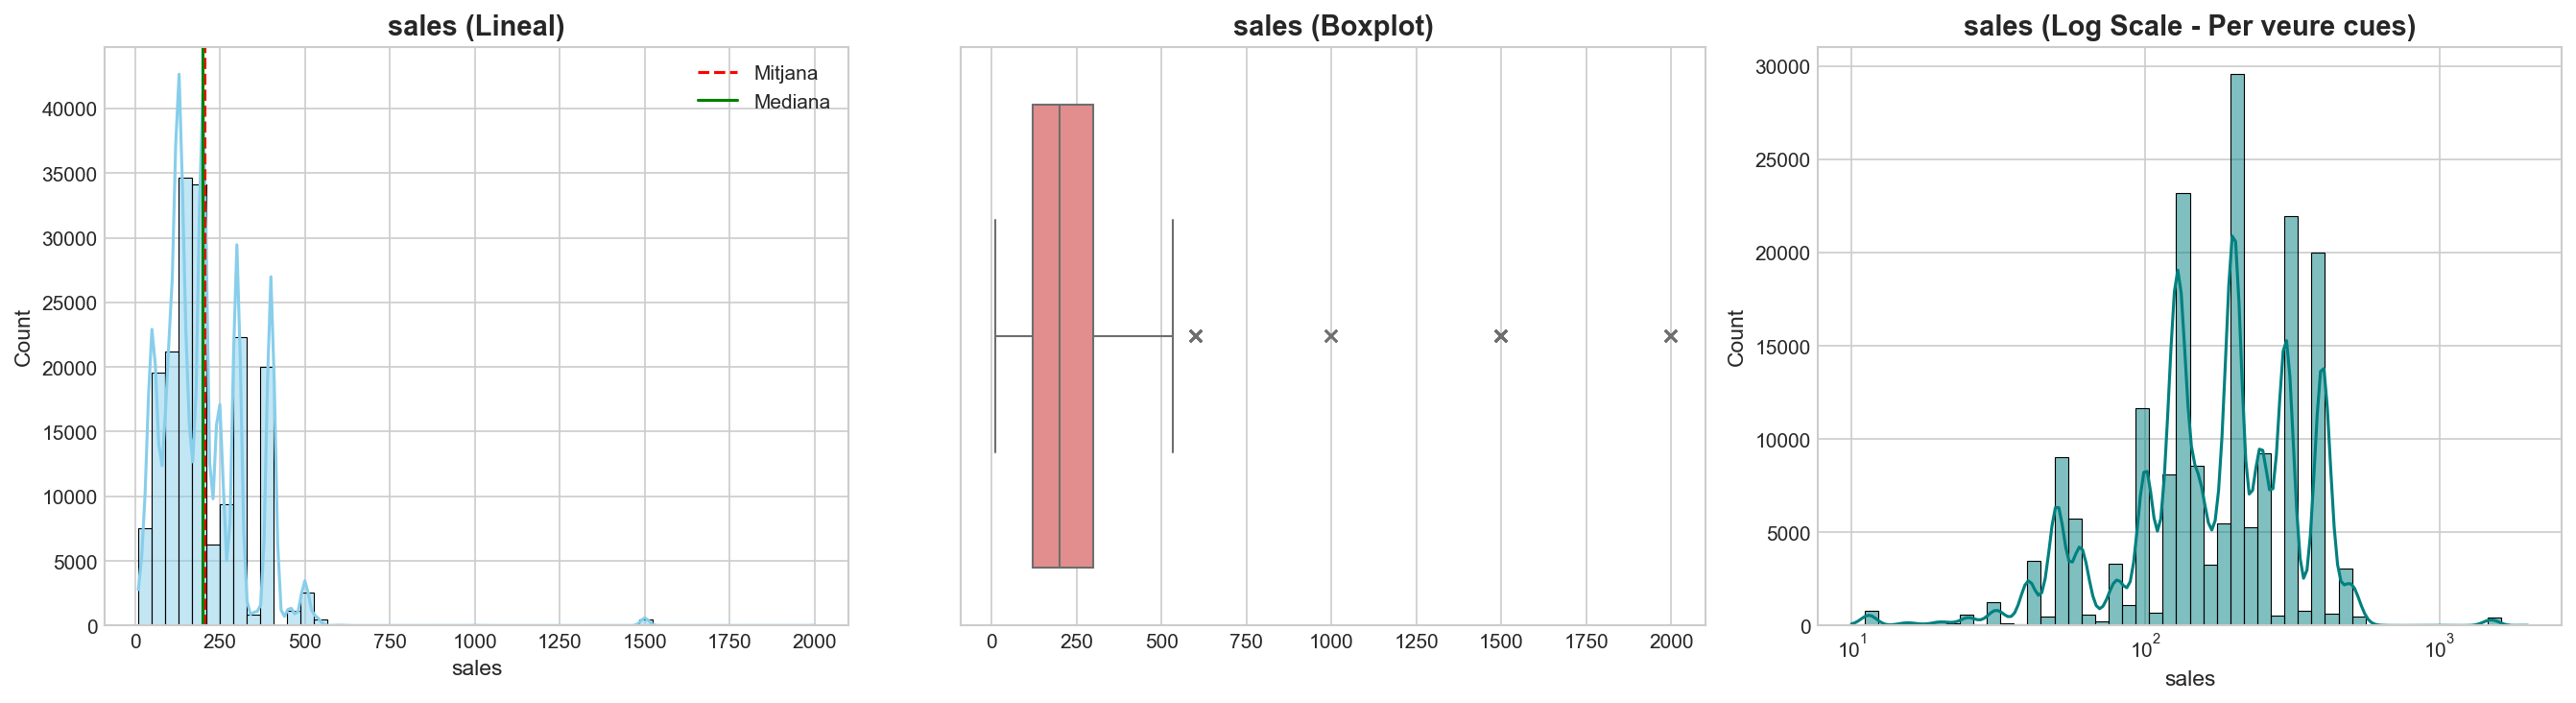
\includegraphics[width=1.0\textwidth]{figures/final/01_univariant/numeriques/num_sales.png}
    \caption{Distribució de les vendes (Escala lineal i logarítmica).}
    \label{fig:sales}
\end{figure}

Tot i que la mitjana de vendes per comanda és de 203.77\$, la presència d'una ''cua llarga'' de comandes d'alt valor estira aquesta xifra cap amunt.

El diagrama de caixa (centre de la Figura \ref{fig:sales}) ens ajuda a acotar la normalitat, mostrant que el 50\% central de les operacions es mou realment entre 80\$ i 350\$, i identificant visualment els valors superiors (les 'X') com a anomalies.

Finalment, la visualització en escala logarítmica (dreta) ens permet apreciar millor aquestes comandes grans que, encara que són menys freqüents, aporten gran part de la facturació.

\newpage
\paragraph{La dualitat del Benefici}
Potser la troballa més crítica és la distribució del benefici (\texttt{benefit\_per\_order}). A diferència de les vendes, aquí trobem una asimetria negativa forta (Skewness: -4.74).

\begin{figure}[H]
    \centering
    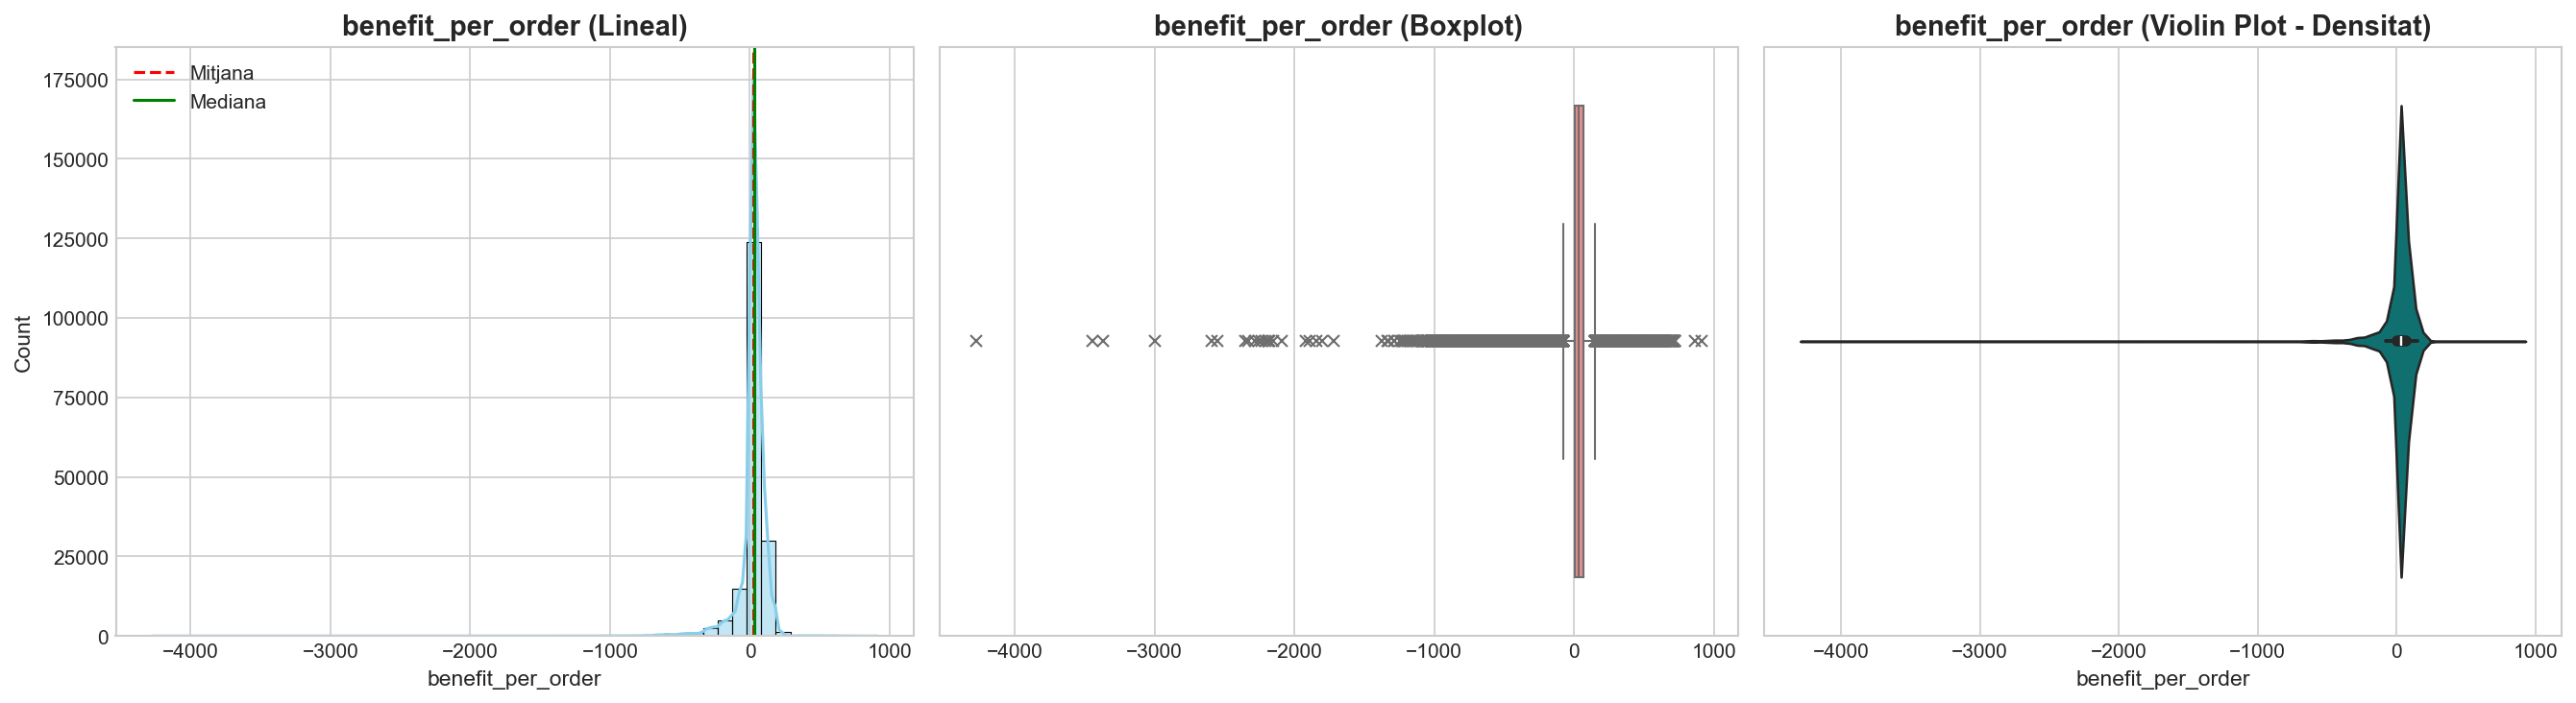
\includegraphics[width=1.0\textwidth]{figures/final/01_univariant/numeriques/num_benefit_per_order.png}
    \caption{Distribució del benefici per comanda. Noteu els valors negatius a l'esquerra.}
    \label{fig:benefit}
\end{figure}

Les dades indiquen que:
\begin{itemize}
    \item \textbf{Marges ajustats:} La mitjana de benefici és baixa (21.97\$) en comparació amb les vendes. La forma punxeguda de l'histograma i la caixa comprimida del Boxplot confirmen que la gran majoria d'operacions tenen un benefici mínim, proper al punt d'equilibri.
    
    \item \textbf{Pèrdues severes (Cua Esquerra):} Existeix una quantitat significativa d'operacions amb rendibilitat negativa. A diferència de les vendes, el Boxplot mostra \textit{outliers} que s'estenen dramàticament cap a l'esquerra (fins a -4.000\$), indicant operacions puntuals que destrueixen valor.
    
    \item \textbf{Kurtosis extrema (71.38):} Aquest valor ens avisa que tenim cues molt pesades. Ens indica que, fora de la normalitat, els casos són extrems: o es guanya bastant o, més preocupantment, es perd molt, sense gaires ''termes mitjos''.
\end{itemize}

Això ens porta a plantejar la hipòtesi per a l'anàlisi bivariant: \textit{Què està causant aquestes pèrdues? Són descomptes excessius o costos d'enviament mal calculats?}

\paragraph{Anàlisi dels retards (Dies)}
Finalment, quantificant el problema logístic, veiem que la mitjana de dies reals d'enviament (3.50 dies) supera sistemàticament la mitjana programada (2.93 dies). El retard mitjà (\texttt{delay\_days}) és de 0.57 dies, però amb una desviació estàndard alta (1.49), fet que explica la impredictibilitat del servei.
\newpage

% ============================================================================
% 5.3 ANÀLISI BIVARIANT
% ============================================================================
\subsection{Anàlisi Bivariant}

En aquesta fase, hem creuat les variables clau per entendre les causes dels fenòmens detectats anteriorment, especialment els retards i la variabilitat del benefici.

\subsubsection{La paradoxa de l'eficiència logística}
Hem analitzat la relació entre el mode d'enviament (\texttt{shipping\_mode}) i els dies de retard (\texttt{delay\_days}). Els resultats, validats pel test de Kruskal-Wallis (p < 0.05), mostren una realitat contraintuïtiva il·lustrada a la Figura \ref{fig:ship_delay}.

\begin{figure}[H]
    \centering
    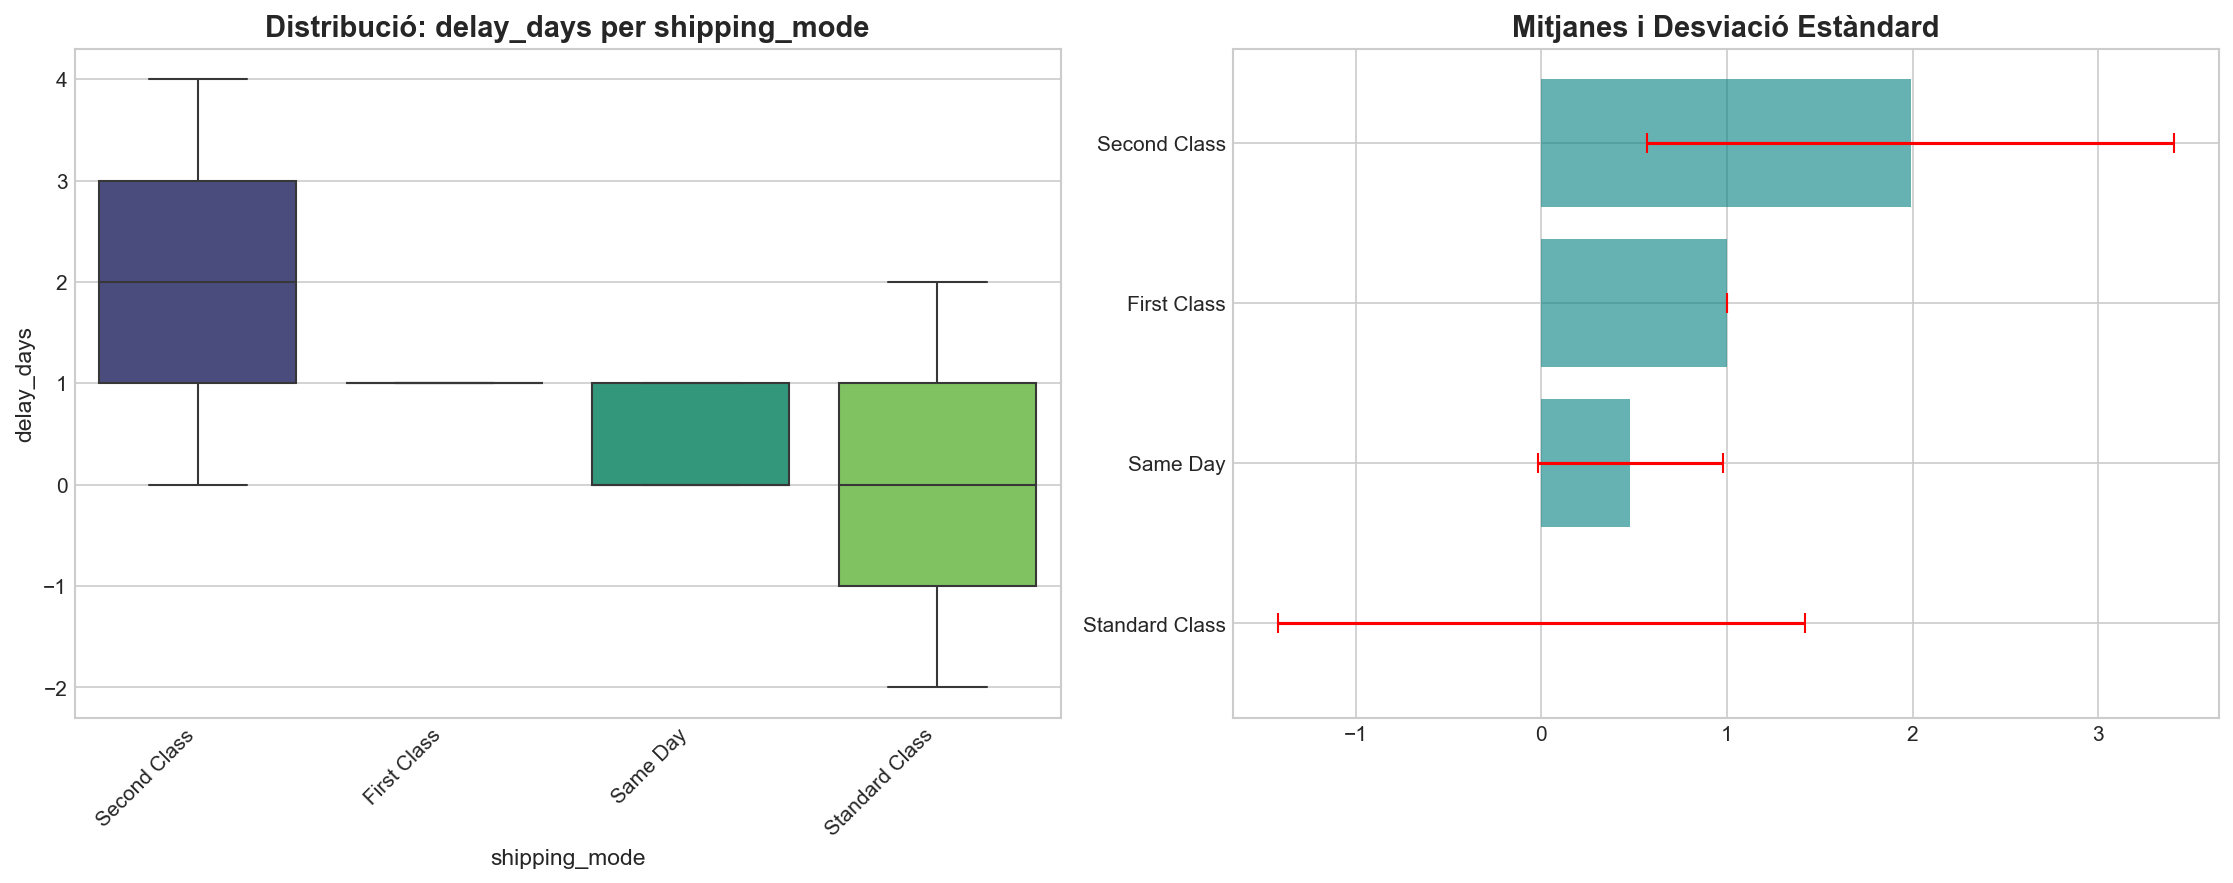
\includegraphics[width=0.9\textwidth]{figures/final/02_bivariant/cat_vs_num/shipping_mode_vs_delay_days.png}
    \caption{Distribució de dies de retard per mode d'enviament.}
    \label{fig:ship_delay}
\end{figure}

Com es detalla a la Taula \ref{tab:shipping_delay}, ens trobem davant d'una paradoxa operativa: els mètodes d'enviament suposadament més ràpids i prèmium són els que acumulen més retard respecte a la data promesa.

\begin{table}[H]
\centering
\caption{Estadístics de retard segons mode d'enviament}
\label{tab:shipping_delay}
\begin{tabular}{lrrr}
\toprule
\textbf{Mode d'Enviament} & \textbf{N} & \textbf{Retard Mitjà (dies)} & \textbf{Desv. Std} \\
\midrule
Standard Class & 107,752 & \textbf{-0.00} & 1.42 \\
Same Day & 9,737 & 0.48 & 0.50 \\
First Class & 27,814 & 1.00 & 0.00 \\
Second Class & 35,216 & \textbf{1.99} & 1.42 \\
\bottomrule
\end{tabular}
\end{table}

L'anàlisi revela dos comportaments oposats:
\begin{itemize}
    \item La \textbf{Standard Class} presenta una mitjana perfecta (-0.00), però la seva alta desviació estàndard (1.42) i la distribució del \textit{boxplot} indiquen que això s'aconsegueix gràcies a paquets que arriben \textbf{abans d'hora} (valors negatius), compensant els que arriben tard.
    \item La \textbf{Second Class}, en canvi, és sistemàticament la menys eficient, amb un retard mitjà de gairebé 2 dies.
    \item La \textbf{First Class} mostra un comportament rígid amb un retard constant d'1 dia (Desv. Std 0.00).
\end{itemize}

Aquestes dades suggereixen que l'empresa promet terminis massa ajustats o impossibles per als serveis prèmium, mentre que és massa conservadora amb l'estàndard, generant una potencial frustració en el client que paga un extra per rapidesa i rep un servei pitjor.
\subsubsection{Rendibilitat per Categoria i Mercat}
Què impulsa realment el benefici? Hem creuat el benefici per comanda amb les categories de producte i els mercats per identificar on es genera valor i on es destrueix.

\paragraph{Categories: El dilema entre rendibilitat i risc}
L'anàlisi revela una dispersió del benefici enorme. La categoria \textit{Fishing} (Pesca) és, amb diferència, la més rendible, amb un benefici mitjà de \textbf{43.65\$}, més del triple que categories tecnològiques com \textit{Electronics} (12.96\$).

No obstant això, la visualització de les desviacions estàndard (Figura \ref{fig:cat_benefit}, dreta) exposa una realitat preocupant:
\begin{itemize}
    \item \textbf{Alta Volatilitat en Productes Estrella:} Les categories més rendibles (\textit{Fishing}, \textit{Camping}) són també les més inestables. Les seves barres d'error són molt àmplies, indicant que, tot i que la mitjana és alta, els resultats varien dràsticament entre comandes.
    \item \textbf{Pèrdues Estructurals:} El \textit{boxplot} (esquerra) mostra que \textbf{totes} les categories, sense excepció, tenen bigotis inferiors que arriben a valors negatius significatius. Això confirma que el problema de les pèrdues no és específic d'un mal producte, sinó un problema operatiu transversal (devolucions o costos logístics) que afecta tot el catàleg.
\end{itemize}

\begin{figure}[H]
    \centering
    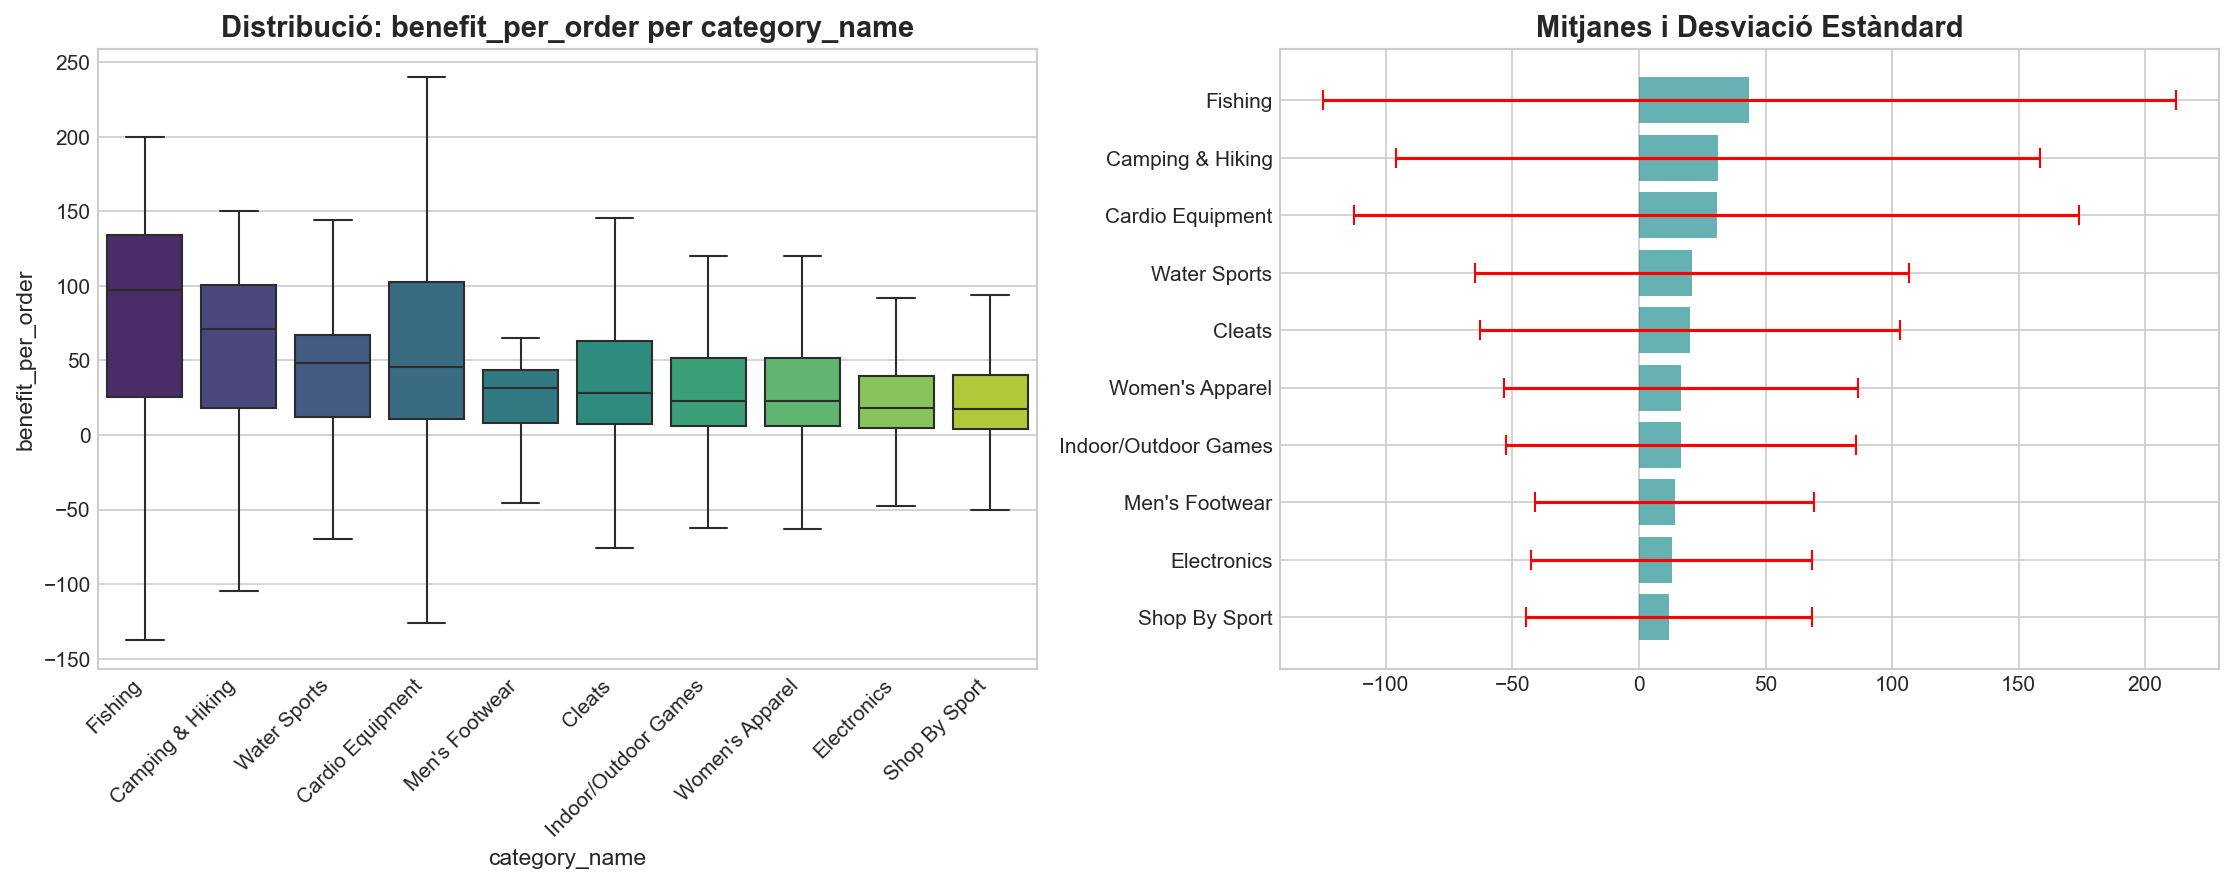
\includegraphics[width=0.9\textwidth]{figures/final/02_bivariant/cat_vs_num/category_name_vs_benefit_per_order.png}
    \caption{Benefici per comanda: Distribució i Volatilitat per Categoria.}
    \label{fig:cat_benefit}
\end{figure}

\paragraph{Mercats més valuosos}
Des d'una perspectiva geogràfica, Europa es posiciona com el mercat amb el tiquet mitjà (Vendes) més alt (\textbf{216.36\$}), significativament superior als EUA (USCA) que es queda en 196.38\$. Aquesta diferència, validada estadísticament ($p < 0.05$), suggereix que el client europeu tendeix a fer cistelles de compra més grans, fet que podria amortitzar millor els costos d'enviament fixos si la logística es gestiona correctament.

\subsubsection{Anàlisi de Segments: Un resultat negatiu rellevant}
És important destacar un ''no-resultat'' que té grans implicacions estratègiques. En analitzar el benefici segons el segment de client (\texttt{customer\_segment}), el test de Kruskal-Wallis ha donat un \textit{p-valor} de 0.165 (no significatiu), indicant una manca de diferències reals entre grups.

\begin{figure}[H]
    \centering
    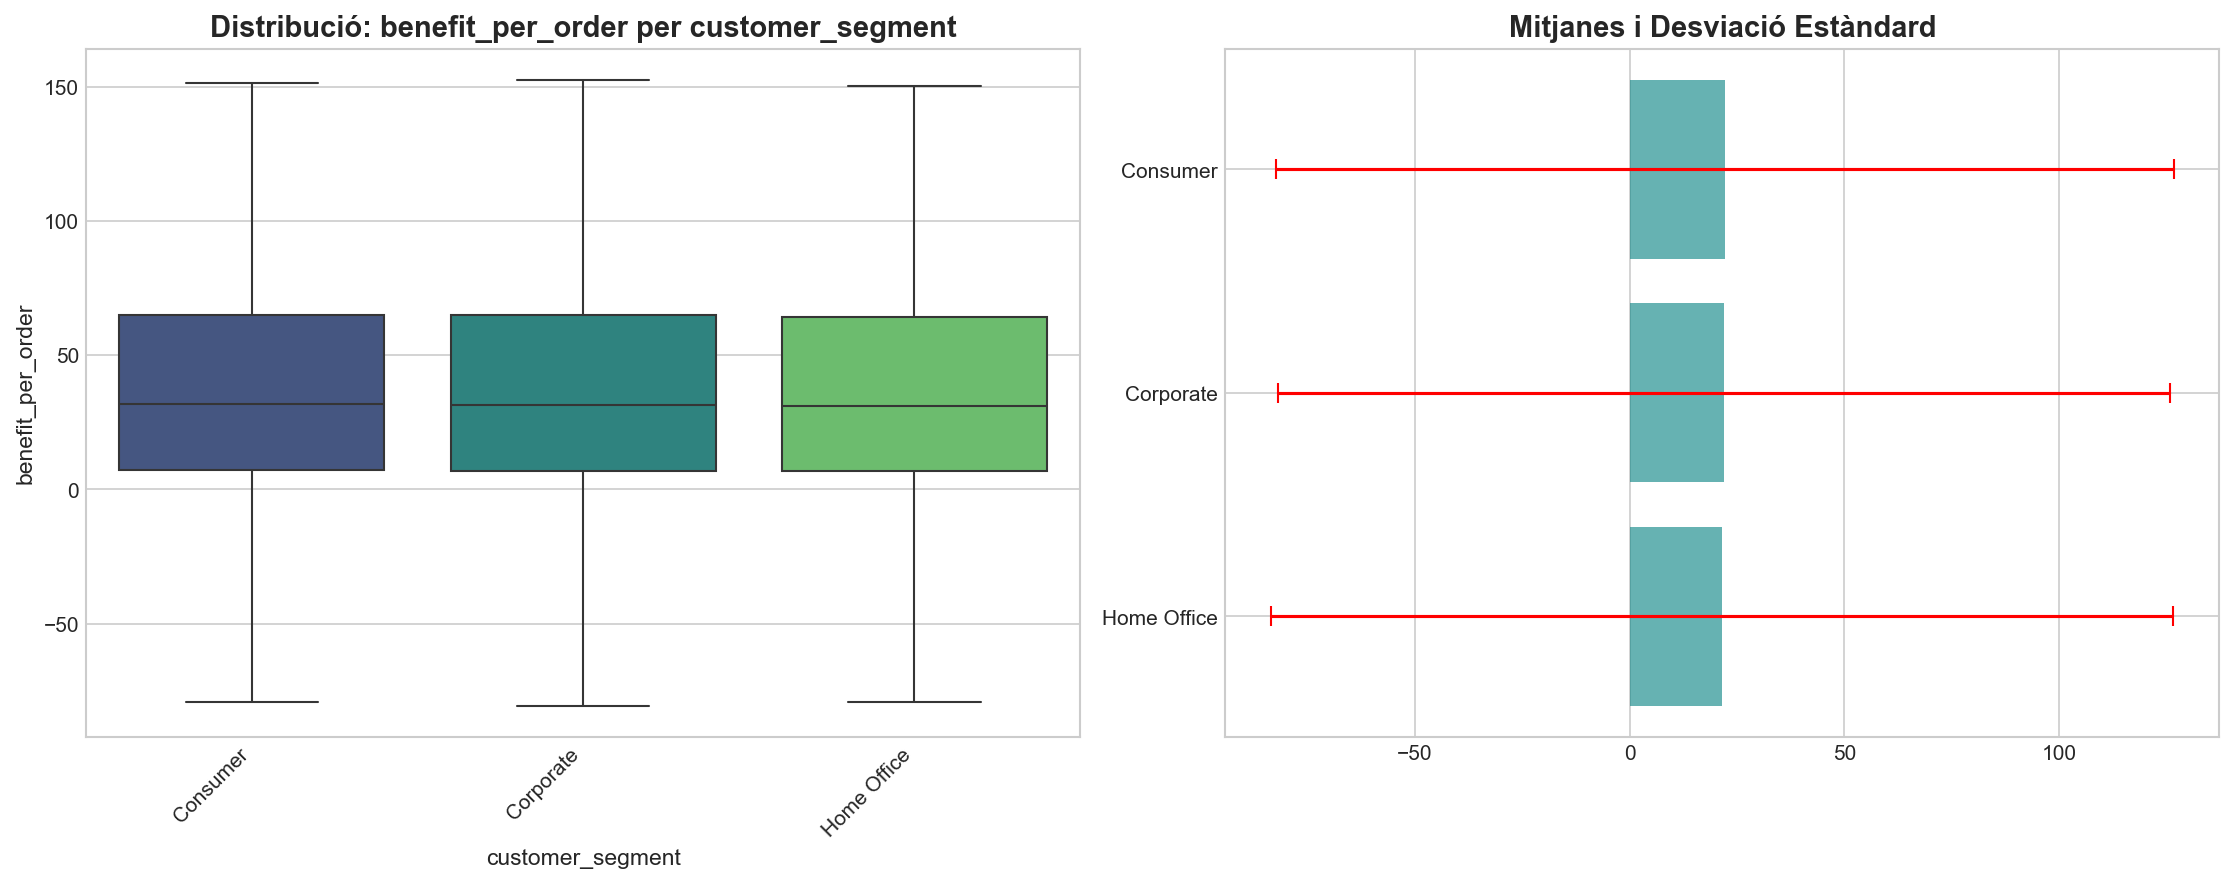
\includegraphics[width=0.8\textwidth]{figures/final/02_bivariant/cat_vs_num/customer_segment_vs_benefit_per_order.png}
    \caption{Comparació de benefici entre segments de clients.}
    \label{fig:cust_seg}
\end{figure}

Com es detalla a la Taula \ref{tab:segment_stats}, les mètriques són sorprenentment uniformes. Tant els clients particulars (\textit{Consumer}) com els corporatius (\textit{Corporate}) aporten el mateix benefici mitjà (~22\$) i, el més important, comparteixen el mateix nivell de risc, amb una desviació estàndard extremadament alta (~104\$).

\begin{table}[H]
\centering
\caption{Estadístics de Benefici per Segment de Client}
\label{tab:segment_stats}
\begin{tabular}{lrrrr}
\toprule
\textbf{Segment} & \textbf{N} & \textbf{Mitjana (\$)} & \textbf{Mediana (\$)} & \textbf{Desv. Std} \\
\midrule
Consumer & 93,504 & 22.18 & 31.85 & 104.54 \\
Corporate & 54,789 & 21.95 & 31.32 & 103.87 \\
Home Office & 32,226 & 21.44 & 31.11 & 105.08 \\
\bottomrule
\end{tabular}
\end{table}

\textbf{Conclusió de negoci:} Aquesta homogeneïtat implica que estratègies de màrqueting basades en tractar el client corporatiu com a ''VIP'' o més rendible no tenen base financera en aquest dataset. El problema de la volatilitat dels beneficis és estructural i no depèn de qui fa la compra.
\subsubsection{Anàlisi de Risc: La probabilitat de retard}
L'anàlisi anterior mostrava el retard mitjà, però per prendre decisions operatives necessitem entendre quantes comandes arriben tard (probabilitat de fallada). Per això, hem calculat el percentatge de comandes amb retard segons el mode d'enviament.

Els resultats de la Figura \ref{fig:risk_ship} són alarmants i confirmen la ineficiència dels serveis ràpids.

\begin{figure}[H]
    \centering
    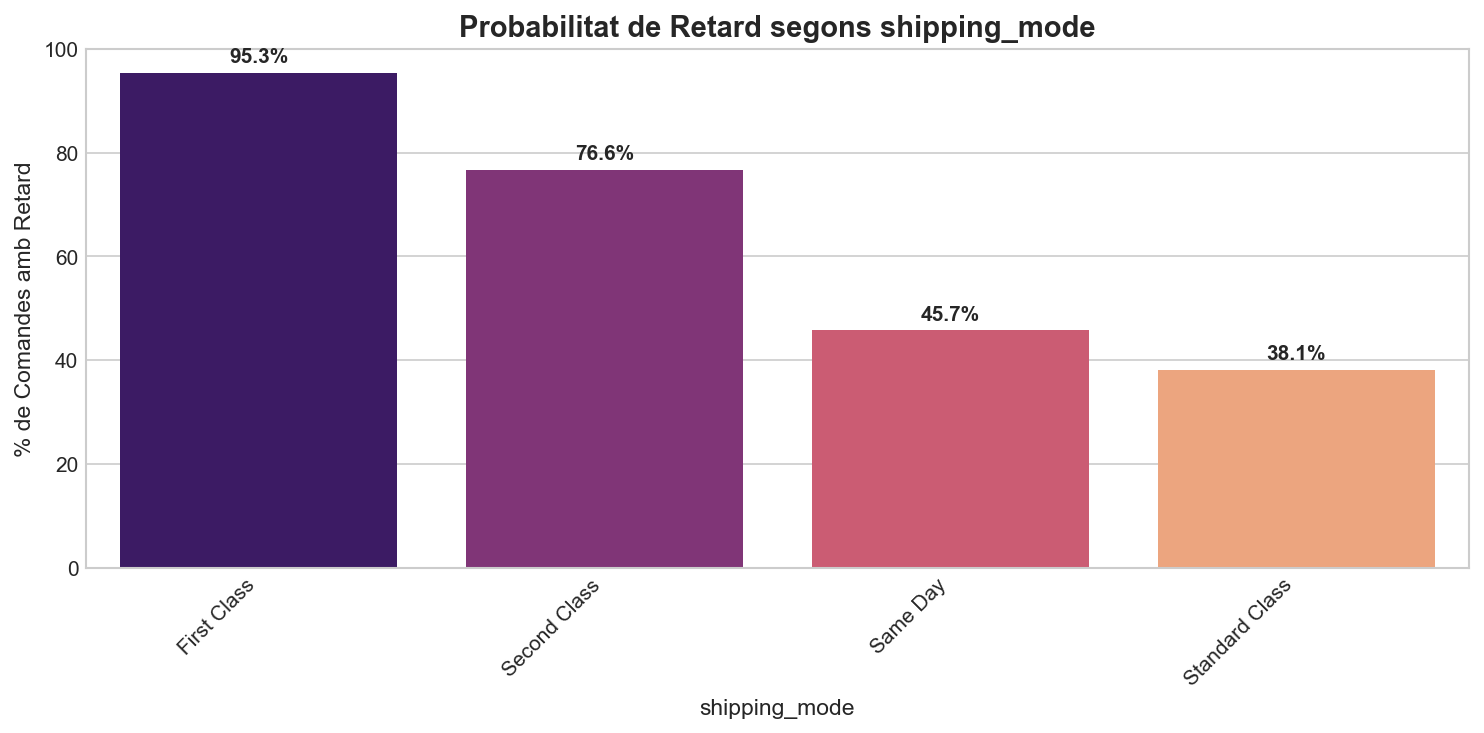
\includegraphics[width=0.8\textwidth]{figures/final/02_bivariant/cat_vs_cat/risk_shipping_mode.png}
    \caption{Percentatge de comandes amb retard segons el mode d'enviament.}
    \label{fig:risk_ship}
\end{figure}

Mentre que l'anàlisi per mercats o segments de client mostra un risc homogeni (al voltant del 55\% a tot arreu), l'anàlisi per mode d'enviament destapa una fallada sistèmica en els serveis prèmium:

\begin{itemize}
    \item \textbf{Fallada gairebé total en First Class:} El 95.3\% de les comandes de ''Primera Classe'' arriben amb retard. Això implica que és pràcticament impossible per a l'empresa complir amb la promesa d'aquest servei.
    
    \item \textbf{Second Class també falla:} El 76.6\% de les comandes de segona classe arriben tard.
    
    \item \textbf{L'opció més segura és la barata:} Paradoxalment, la \textit{Standard Class} és l'opció més fiable, amb només un 38.1\% de probabilitat de retard.
\end{itemize}

\textbf{Conclusió:} Existeix una correlació inversa entre el preu de l'enviament i la fiabilitat. Els serveis que haurien de ser prioritaris són els que tenen les taxes de fallada més altes, posant en risc la reputació de l'empresa i la satisfacció dels clients de més valor.

\subsubsection{Correlacions i Vendes: L'estructura del risc}
Finalment, l'anàlisi de dispersió (Figura \ref{fig:scatter}) és fonamental per entendre la qualitat de la facturació.

\begin{figure}[H]
    \centering
    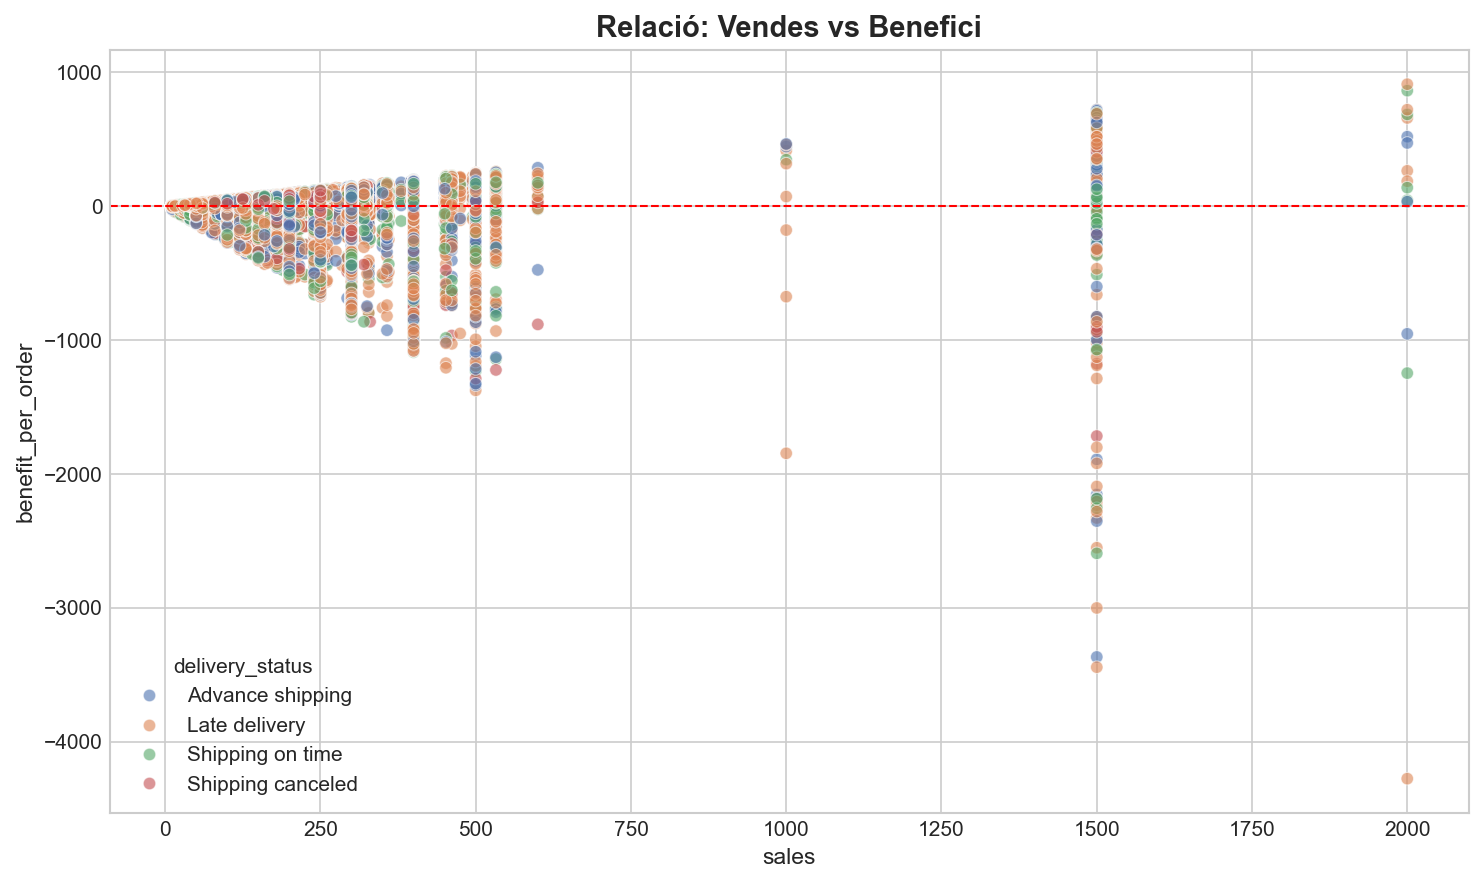
\includegraphics[width=0.8\textwidth]{figures/final/02_bivariant/num_vs_num/scatter_sales_benefit.png}
    \caption{Relació Vendes vs. Benefici. Els colors indiquen l'estat de l'entrega.}
    \label{fig:scatter}
\end{figure}

El gràfic revela tres patrons crítics que confirmen una estructura de risc asimètrica:

\begin{itemize}
    \item \textbf{Heteroscedasticitat (Efecte Ventall):} A mesura que augmenta el volum de vendes (eix X), la variància es dispara. Les operacions de major valor són les més inestables.
    
    \item \textbf{Asimetria Pèrdua-Guany:} Existeix un desequilibri preocupant. Mentre que el benefici màxim per comanda rarament s'apropa als +1.000\$, les pèrdues poden enfonsar-se arribant a superar -4.000\$. Això pot indicar que una mala gestió dels descomptes en productes cars penalitza molt més del que aporta una venda exitosa.
    
    \item \textbf{El paper dels Descomptes vs. Logística:} La distribució aleatòria dels colors (estat d'entrega) suggereix que els problemes logístics no són el detonant directe de les pèrdues financeres. En canvi, la forta correlació entre \textit{Sales} i \textit{Discount} (0.617) apunta a que l'aplicació agressiva de descomptes en comandes grans és la principal destructora de marge.
\end{itemize}

% ============================================================================
% 5.4 ANÀLISI MULTIVARIANT
% ============================================================================
\subsection{Anàlisi Multivariant}

Per tancar l'etapa exploratòria, hem afegit una tercera dimensió a les visualitzacions. Això ens permet verificar si els patrons detectats (com la rendibilitat de certs productes o els retards) són globals o si depenen de la regió geogràfica.

\subsubsection{Mapa de calor: Consistència Global del Producte}
A la secció bivariant havíem vist que la categoria \textit{Fishing} era molt rendible. Ara, creuant \textbf{Categoria vs. Mercat vs. Benefici} (Figura \ref{fig:heatmap}), confirmem que aquesta rendibilitat és estructural del producte i no depèn de la regió.

\begin{figure}[H]
    \centering
    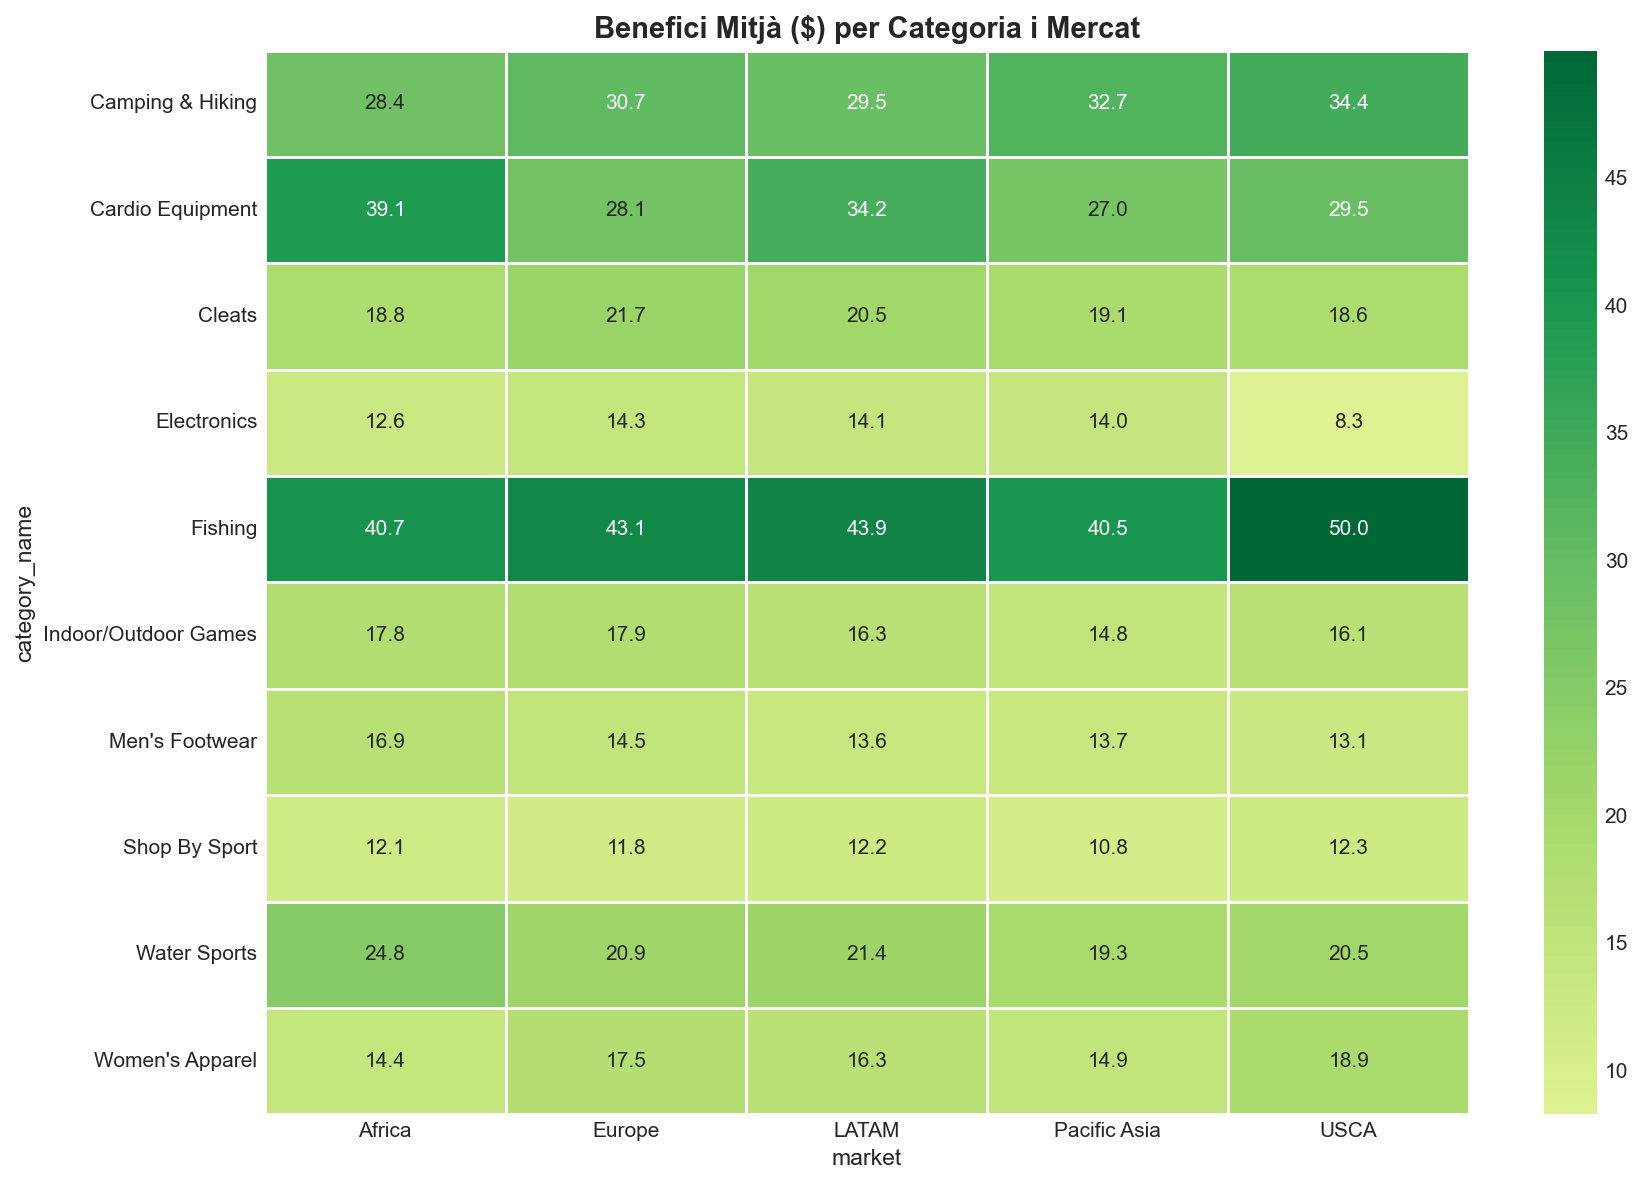
\includegraphics[width=0.95\textwidth]{figures/final/03_multivariant/heatmap_benefit_market_cat.png}
    \caption{Mapa de calor del benefici mitjà per Categoria i Mercat. La intensitat del verd indica alta rendibilitat; els tons grocs, marges ajustats.}
    \label{fig:heatmap}
\end{figure}

El mapa de calor revela una \textbf{jerarquia clara}:
\begin{itemize}
    \item \textbf{Consistència del Producte Estrella:} La categoria \textit{Fishing} es mostra en verd intens a gairebé tots els mercats (superant els 40\$ de mitjana), amb un pic destacat al mercat \textbf{USCA} (50.0\$). Això demostra que és un producte guanyador global.
    
    \item \textbf{Marges Ajustats Transversals:} Per contra, categories com \textit{Electronics} o \textit{Shop By Sport} apareixen en color groc pàl·lid (mitjanes baixes de 10-14\$) a totes les regions. No és un problema específic de LATAM, sinó una característica d'aquests productes que tenen poc marge a tot el món.
    
    \item \textbf{Anomalia Positiva:} Destaca l'excepció de \textit{Cardio Equipment} a l'Àfrica, on mostra un rendiment inusualment alt (39.1\$) comparat amb la resta de continents, suggerint una oportunitat de nínxol en aquest mercat específic.
\end{itemize}
\subsubsection{La universalitat del retard logístic}
Recordem la ''paradoxa logística'' detectada anteriorment, on els enviaments de \textit{Second Class} eren els que més fallavem i els estàndard els que menys. Ens preguntàvem: és un problema d'infraestructura en països concrets? La Figura \ref{fig:delay_region} ofereix una resposta definitiva.

\begin{figure}[H]
    \centering
    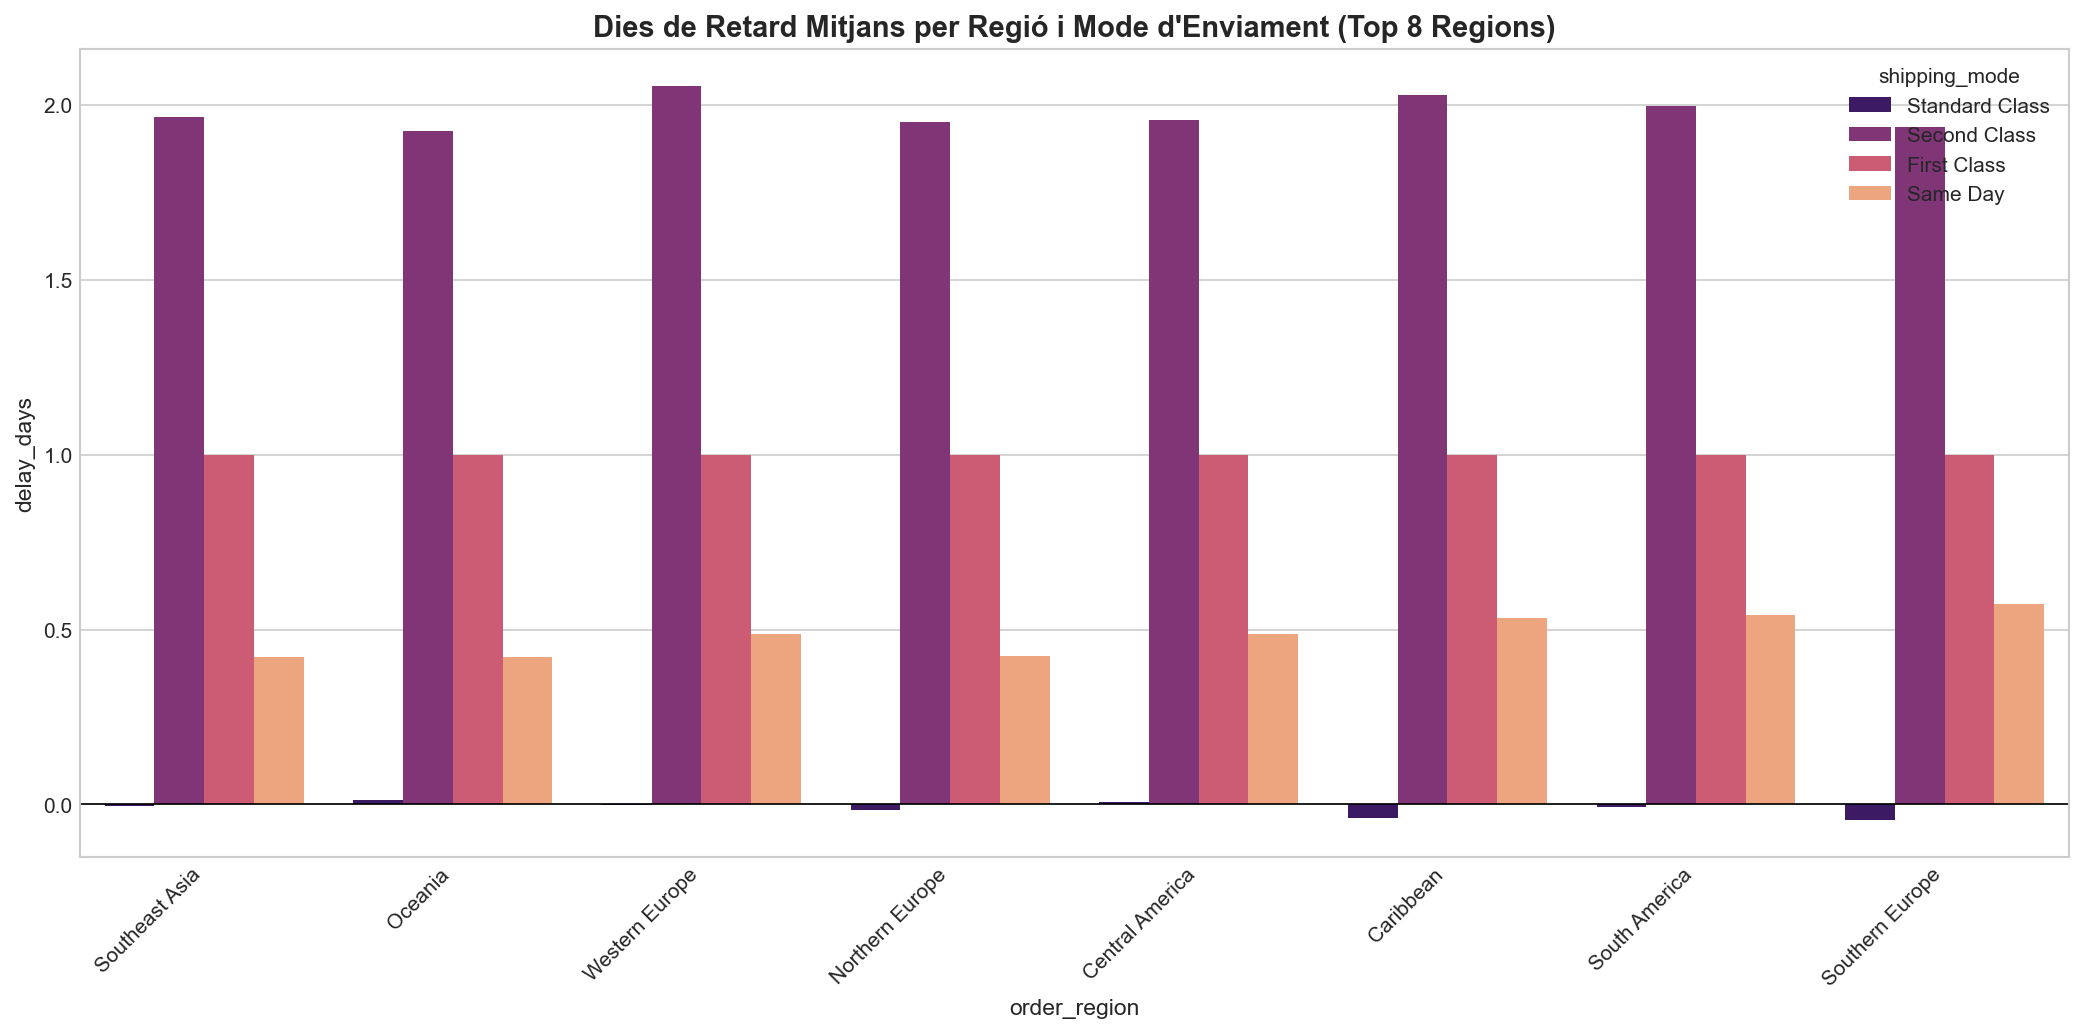
\includegraphics[width=1.0\textwidth]{figures/final/03_multivariant/bar_delay_region_mode.png}
    \caption{Mitjana de dies de retard desglossada per Regió i Mode d'Enviament.}
    \label{fig:delay_region}
\end{figure}

L'anàlisi multivariant revela una invariància geogràfica absoluta. Com s'observa al gràfic, el patró de barres es repeteix com una ''fotocòpia'' a les 8 principals regions comercials (des d'Europa fins a Sud-amèrica):

\begin{itemize}
    \item \textbf{Consistència del Fracàs:} La barra lila (\textit{Second Class}) és sistemàticament la més alta a totes les regions, amb un retard mitjà clavat al voltant dels \textbf{2 dies}. De la mateixa manera, la \textit{First Class} (rosa) manté un retard constant d'1 dia globalment.
    \item \textbf{L'excepció positiva:} La \textit{Standard Class} (barra fosca) es manté invisible o propera a 0 a tot el món, demostrant ser l'única opció fiable independentment del destí.
\end{itemize}

\textbf{Conclusió:} Aquesta homogeneïtat descarta la hipòtesi de problemes en duanes locals o infraestructures regionals. El problema és \textbf{sistèmic i centralitzat}: l'empresa (o el seu operador logístic global) està calculant erròniament les dates d'entrega promesa per als serveis prèmium a escala mundial, generant expectatives impossibles de complir a qualsevol continent.
\subsubsection{Impacte dels descomptes per mercat: Risc global compartit}
Finalment, la Figura \ref{fig:scatter_discount} explora si la sensibilitat als descomptes varia segons la regió geogràfica.

\begin{figure}[H]
    \centering
    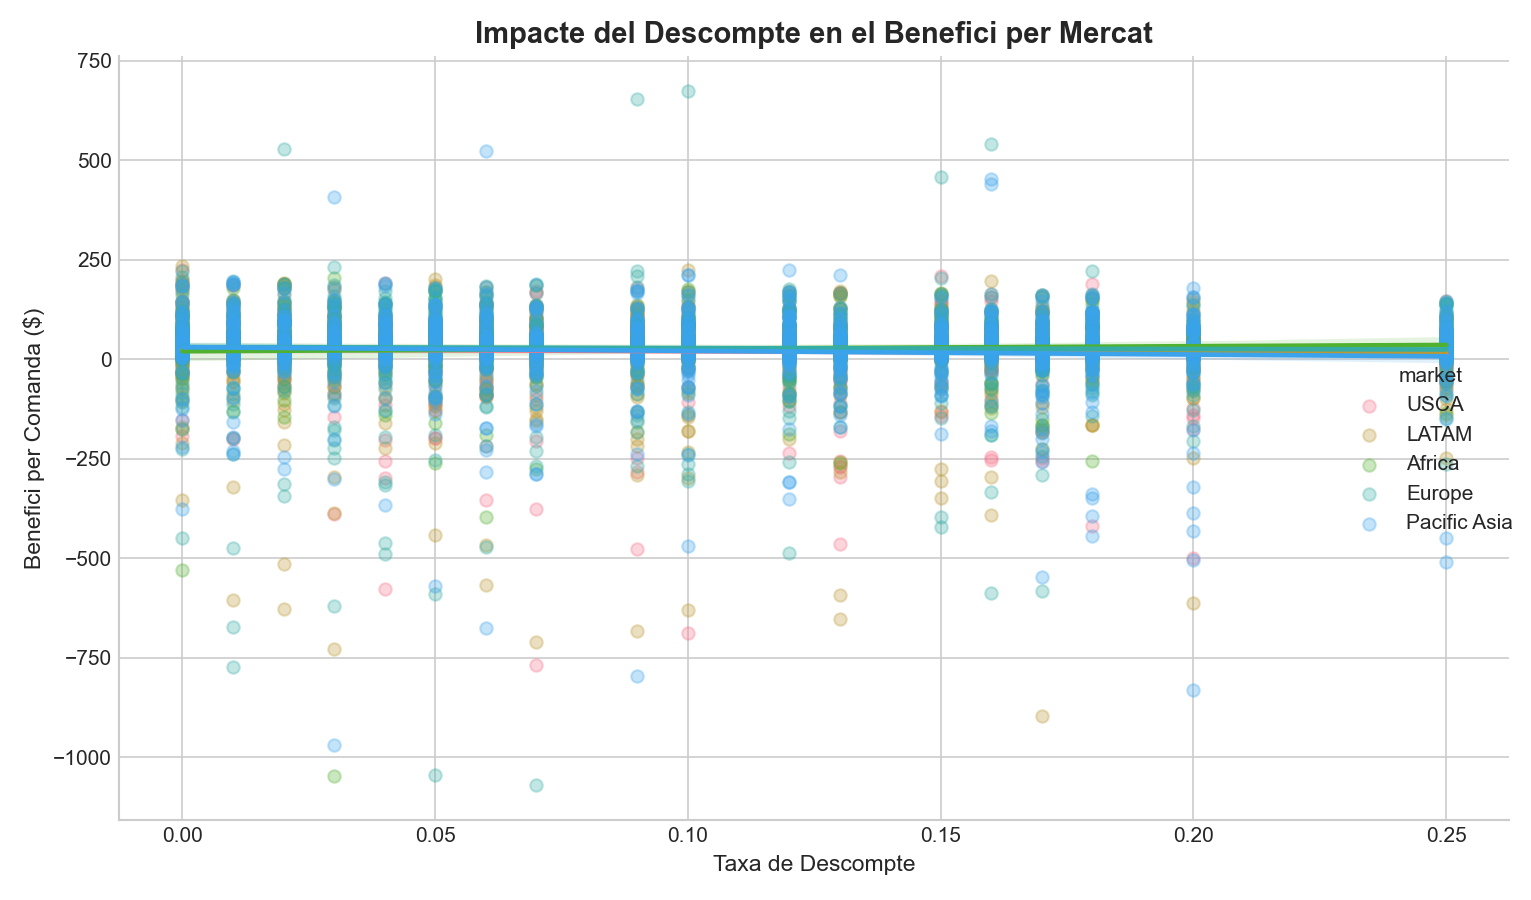
\includegraphics[width=0.85\textwidth]{figures/final/03_multivariant/scatter_discount_benefit_market.png}
    \caption{Relació entre taxa de descompte i benefici. Els punts per sota de 0 indiquen comandes amb pèrdues.}
    \label{fig:scatter_discount}
\end{figure}

El gràfic revela dos patrons clau per a la presa de decisions:

\begin{itemize}
    \item \textbf{Homogeneïtat de Mercat:} Les línies de tendència de tots els mercats (Europa, LATAM, USCA, etc.) es superposen i són pràcticament idèntiques. Això significa que no hi ha cap regió ''immune'' als descomptes; l'elasticitat del preu és universal i, per tant, la política de descomptes ha de ser global i centralitzada.
    
    \item \textbf{Descomptes i Pèrdues:} Tot i que la mitjana (línies rectes) es manté estable prop de zero, observem una gran dispersió de punts individuals cap a la zona negativa (valors de -250\$ a -1.000\$). Això confirma que, encara que el promig no s'enfonsi, l'aplicació de descomptes (especialment els superiors al 10\%) augmenta dràsticament el risc d'incórrer en pèrdues severes en operacions concretes, independentment del mercat.
\end{itemize}
% ============================================================================
% 5.5 ESTUDIS ESPECÍFICS
% ============================================================================
\subsection{Estudis específics d'aprofundiment}

Més enllà de la descripció estadística estàndard, hem volgut aplicar tècniques avançades (Machine Learning i simulació) per respondre a tres problemes estratègics crítics que hem detectat durant l'exploració: la concentració de risc en el catàleg, la manca de segmentació de clients i la incertesa sobre la rendibilitat dels descomptes.

\subsubsection{Anàlisi de Pareto: Una dependència excessiva de pocs productes}
Hem aplicat la Llei de Pareto (80/20) per veure si les vendes estan ben repartides entre els productes o si depenem massa d'uns pocs. El resultat és clar: la concentració és molt més alta del que seria saludable.

\paragraph{7 productes aguanten l'empresa}
Si mirem la corba de la (Figura \ref{fig:pareto}), veiem una dada impactant: de tot el catàleg de 118 productes, \textbf{només 7 generen el 80\% de tots els ingressos}.
En lloc de la famosa proporció 80/20, aquí tenim un 80/6 (7 productes corresponen al 6\% del catàleg). Això vol dir que la immensa majoria del catàleg (més de 100 productes) aporta molt pocs diners a la caixa.

Si baixem al detall dels productes (gràfic de barres dret):
\begin{itemize}
    \item \textbf{El líder indiscutible:} El producte \textit{Field \& Stream Sportsman} factura, ell sol, 6.9 milions de dòlars. Això representa gairebé el \textbf{19\% de tota la facturació} de l'empresa.
    \item \textbf{Marques clau:} Els productes més venuts són de marques molt concretes com \textit{Nike} o \textit{Perfect Fitness}. Si sumem els ingressos dels 4 o 5 primers productes, ja tenim gran part de l'any fet.
\end{itemize}

\begin{figure}[H]
    \centering
    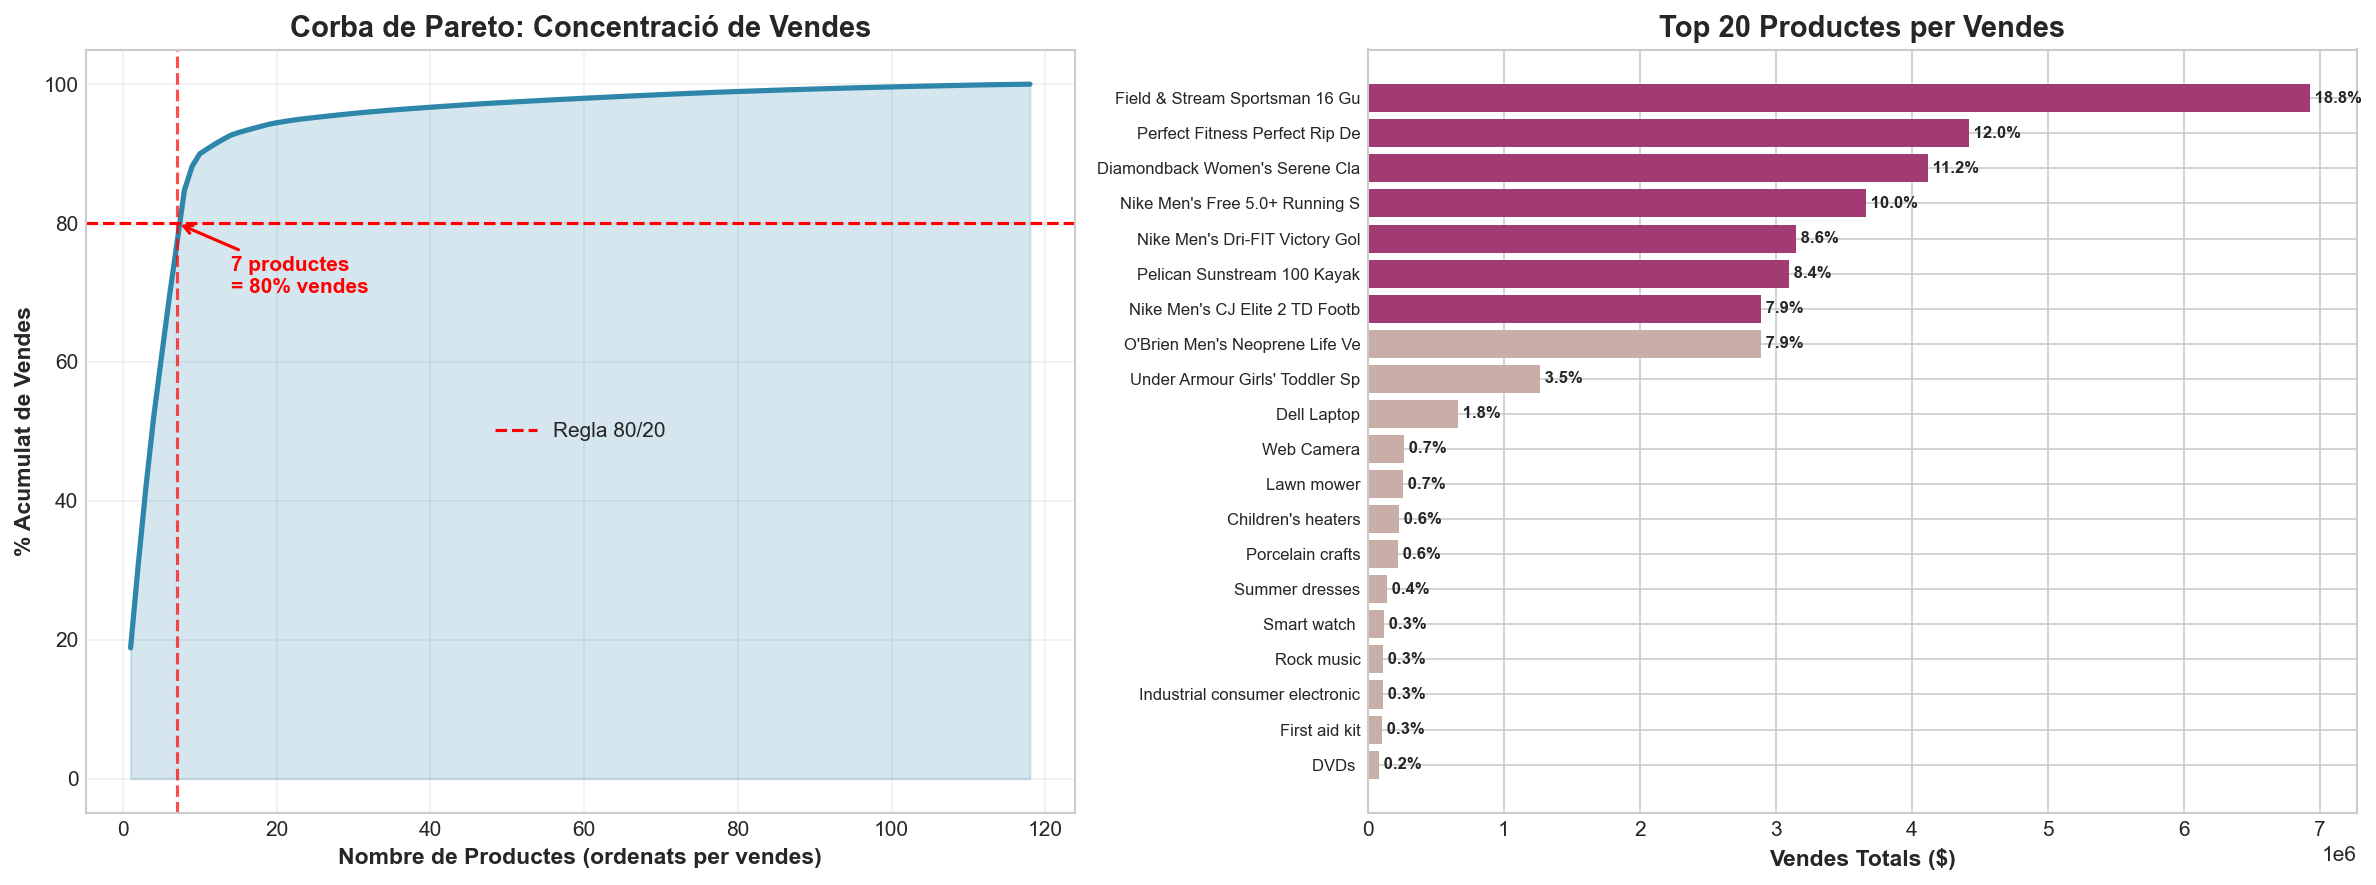
\includegraphics[width=1.0\textwidth]{figures/final/04_estudis_especifics/pareto_products.png}
    \caption{Esquerra: Corba de concentració (amb 7 productes ja fem el 80\% de les vendes). Dreta: Els productes que més facturen.}
    \label{fig:pareto}
\end{figure}

\paragraph{Evolució: Estem anant a pitjor?}
Al gràfic temporal (Figura \ref{fig:pareto_evo}) hem analitzat quants productes feien falta cada any per arribar a aquest 80\% de vendes.
\begin{itemize}
    \item Fins al 2017, la tendència era positiva: cada cop teníem més productes ''importants'' (el pic arriba a 13 productes), cosa que indicava que estàvem diversificant bé.
    \item Però el \textbf{2018 hi ha una caiguda dràstica}. Hem passat a dependre de només 2 o 3 productes per mantenir el gruix del negoci. Això és un senyal d'alerta important.
\end{itemize}

\begin{figure}[H]
    \centering
    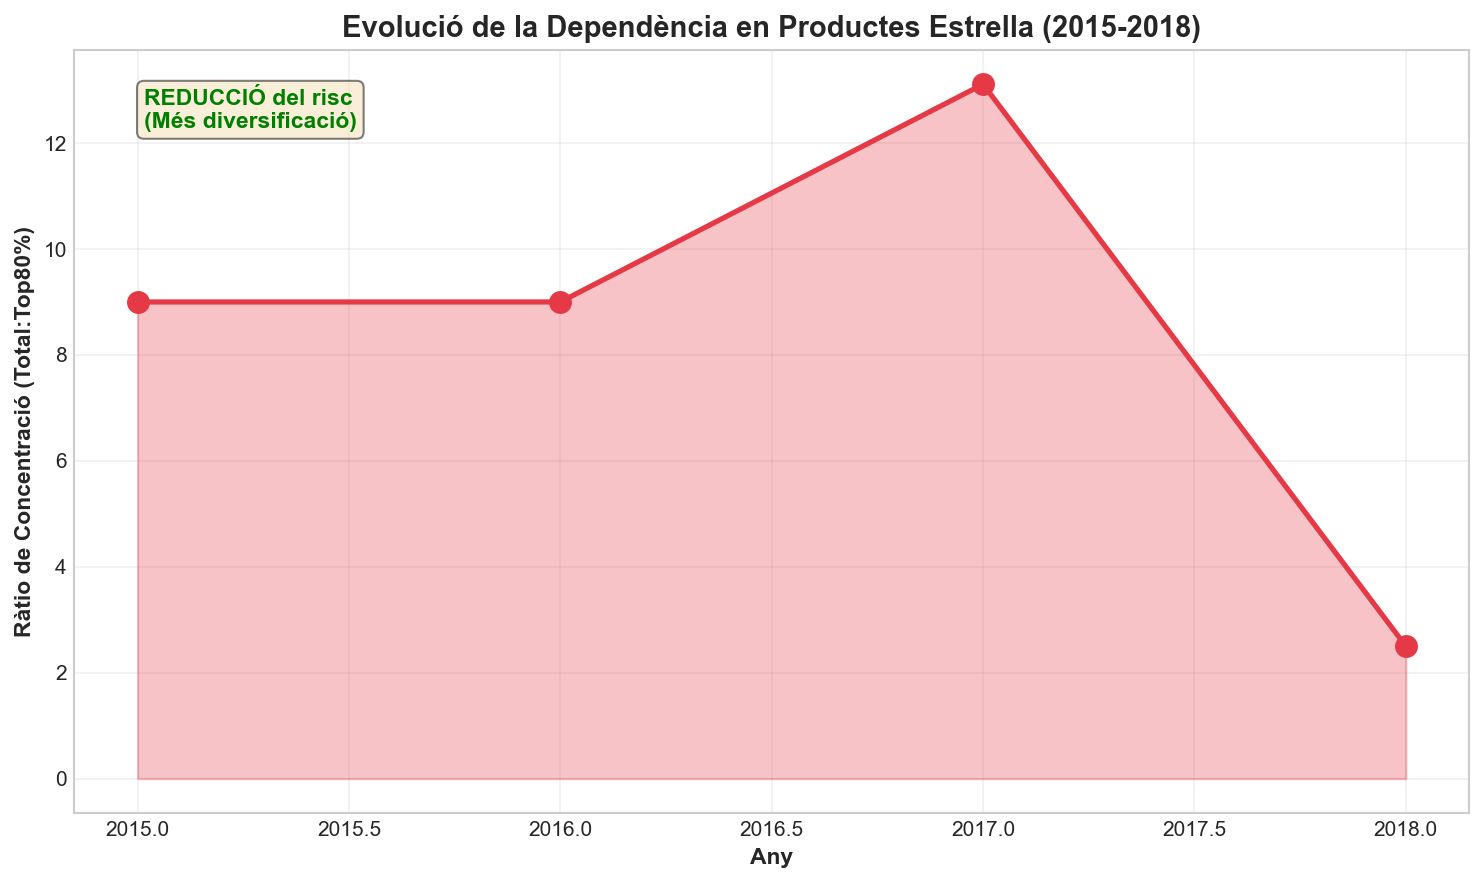
\includegraphics[width=0.8\textwidth]{figures/final/04_estudis_especifics/pareto_evolution.png}
    \caption{Evolució de quants productes calen per arribar al 80\% de les vendes (2015-2018).}
    \label{fig:pareto_evo}
\end{figure}

\paragraph{Per què això és un problema?}
Tenir una dependència tan forta de tan pocs productes ens fa molt fràgils:
\begin{enumerate}
    \item \textbf{Risc d'estoc:} Si el proveïdor de \textit{Nike} falla o tenim un trencament d'estoc amb el \textit{Field \& Stream}, les vendes globals cauran en picat immediatament perquè no tenim altres productes que compensin la pèrdua.
    \item \textbf{Competència:} Si la competència treu un producte millor que el nostre ''Top 1'', l'impacte en els nostres comptes serà enorme.
\end{enumerate}


\subsubsection{Segmentació Avançada de Clients: Model RFM i Clustering}

Fins ara, hem analitzat l'empresa de manera descriptiva (què ha passat). En aquesta secció, fem un salt cap a l'analítica avançada per entendre el comportament dels usuaris.

Per tal de no tractar tots els clients per igual, hem aplicat la metodologia RFM, un estàndard en màrqueting analític que classifica els clients basant-se en tres variables clau:
\begin{itemize}
    \item \textbf{Recència (R):} Quants dies han passat des de l'última compra? (Menys és millor: indica un client actiu).
    \item \textbf{Freqüència (F):} Quantes vegades ha comprat el client? (Més és millor: indica fidelitat).
    \item \textbf{Valor Monetari (M):} Quant ha gastat en total? (Més és millor: indica valor per a l'empresa).
\end{itemize}

Com que analitzar aquestes tres variables manualment per a 20.652 clients és impossible, hem utilitzat un algorisme d'Intel·ligència Artificial no supervisat anomenat \textbf{K-Means}. Aquest algorisme agrupa matemàticament els clients que s'assemblen entre ells en ''Clústers'' o segments.

\paragraph{1. Determinació del nombre òptim de segments (El mètode del Colze)}
Abans de segmentar, hem de decidir quants grups volem fer. Per fer-ho de manera científica i no arbitrària, utilitzem el ''Mètode del Colze'' (Figura \ref{fig:rfm_method}).

\begin{figure}[H]
    \centering
    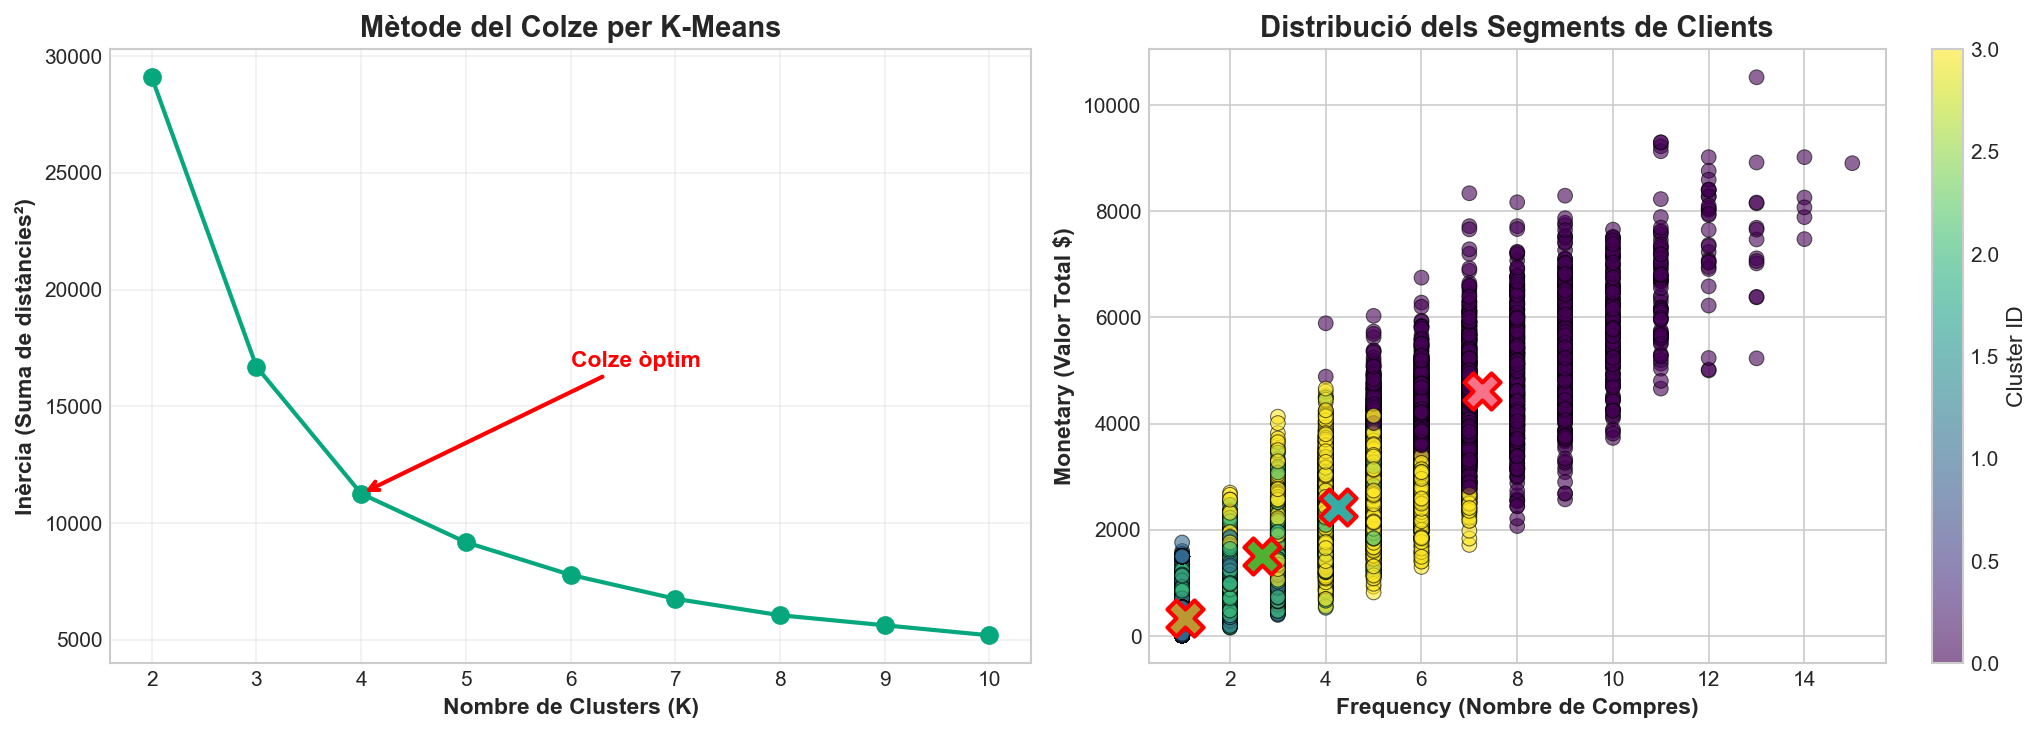
\includegraphics[width=1.0\textwidth]{figures/final/04_estudis_especifics/rfm_clustering.png}
    \caption{Esquerra: Mètode del Colze. L'eix Y (Inèrcia) mesura l'error o la dispersió dins dels grups. Dreta: Visualització dels clústers resultants.}
    \label{fig:rfm_method}
\end{figure}

El gràfic de l'esquerra mostra com es redueix l'error a mesura que afegim més grups. Busquem el punt on la corba fa un ''colze'' (deixa de baixar bruscament i s'estabilitza). En el nostre cas, aquest punt òptim és K=4. Això significa que els nostres clients es divideixen naturalment en 4 grans perfils de comportament.
Aquesta divisió es confirma visualment al gràfic de dispersió de la dreta, on hem projectat els clients segons la seva Freqüència i Valor Monetari:
\begin{itemize}
    \item Els clients (punts) apareixen clarament separats per colors, validant que els grups són diferents entre ells.
    \item Les creus vermelles marquen els ''centroides'': el punt exacte que defineix el comportament mitjà de cada grup.
    \item S'observa una progressió diagonal clara: des de la gran massa de compradors ocasionals (a baix a l'esquerra) fins als clients VIP que compren sovint i gasten molt (a dalt a la dreta).
\end{itemize}

\paragraph{2. Interpretació dels Perfils (Lectura de Boxplots)}
Un cop l'algorisme ha separat els clients en 4 grups (etiquetats del 0 al 3), hem d'entendre ''qui és qui''. Per a això, utilitzem els diagrames de caixa de la Figura \ref{fig:rfm_box}, que ens mostren com es comporta cada grup en les tres variables.

\begin{figure}[H]
    \centering
    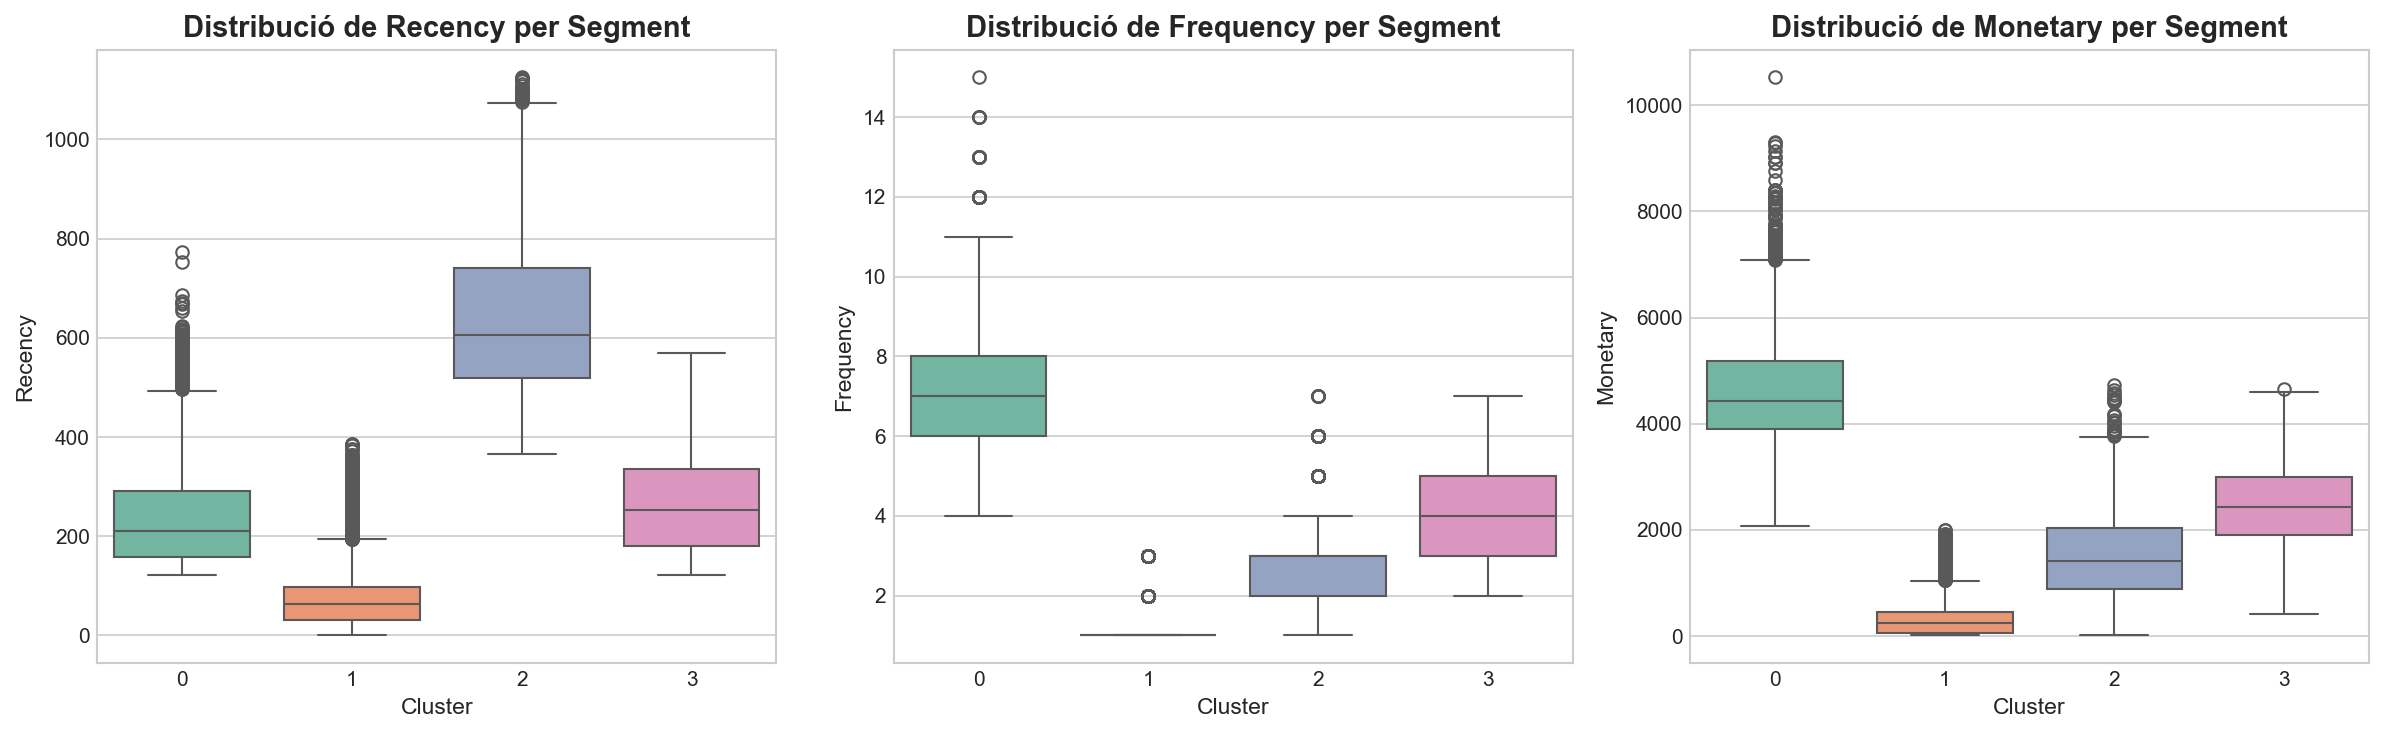
\includegraphics[width=1.0\textwidth]{figures/final/04_estudis_especifics/rfm_boxplots.png}
    \caption{Caracterització dels clústers. Cada color representa un grup de clients i la seva posició indica si tenen valors alts o baixos en Recència, Freqüència i Diners.}
    \label{fig:rfm_box}
\end{figure}

Analitzant els gràfics superiors (Figura \ref{fig:rfm_box}), deduïm la identitat dels 4 segments:

\begin{itemize}
    \item \textbf{Clúster 0 (Caixa Verda):} Els \textbf{Clients VIP}. Destaquen visualment per tenir les caixes més altes en \textit{Frequency} i \textit{Monetary}. Són els que més compren i més gasten.
    
    \item \textbf{Clúster 1 (Caixa Taronja):} Els \textbf{Nous o Ocasionals}. Al primer gràfic (\textit{Recency}), la seva caixa està enganxada a baix de tot (0 dies), cosa que indica que acaben d'arribar i la seva despesa (tercer gràfic) és la més baixa.
    
    \item \textbf{Clúster 2 (Caixa Lila/Blava):} Els \textbf{Inactius o ''Dormits''}. La seva característica definitòria és al primer gràfic: una caixa situada molt amunt (mitjana > 600 dies). Fa anys que no compren i probablement s'han perdut.
    
    \item \textbf{Clúster 3 (Caixa Rosa):} Si mirem els gràfics de \textit{Frequency} i \textit{Monetary}, tenen caixes força altes (bon comportament de compra, gasten uns 2.500\$), però la seva \textit{Recency} és moderada-alta. Són bons clients que s'estan ''refredant''.
\end{itemize}

\paragraph{3. Resultats i Estratègia}
La Taula \ref{tab:rfm_results} resumeix les dades exactes d'aquests perfils i proposa una acció de negoci per a cadascun.

\begin{table}[H]
\centering
\caption{Perfils de Clients i Accions Recomanades}
\label{tab:rfm_results}
\resizebox{\textwidth}{!}{%
\begin{tabular}{llcccc}
\toprule
\textbf{Segment} & \textbf{Descripció} & \textbf{Clients (\%)} & \textbf{Despesa Mitjana} & \textbf{Dies sense comprar} & \textbf{Acció Estratègica} \\
\midrule
\textbf{0 (VIPs)} & Els millors clients & 16.1\% & \$4,626 & 239 dies & Programes de fidelització exclusius. \\
\textbf{3 (Risc)} & Alt valor, però es refreden & \textbf{29.4\%} & \textbf{\$2,437} & \textbf{265 dies} & \textbf{Campanyes de reactivació urgents.} \\
\textbf{1 (Nous)} & Poca despesa, molt recents & 43.0\% & \$335 & 69 dies & Cross-selling per augmentar tiquet. \\
\textbf{2 (Perduts)} & Fa anys que no compren & 11.5\% & \$1,514 & 642 dies & Minimitzar inversió en màrqueting. \\
\bottomrule
\end{tabular}
}
\end{table}

\textbf{Conclusió Clau:} L'anàlisi ha revelat l'existència del \textbf{Segment 3 (Potencials en Risc)}. Aquest grup representa gairebé el 30\% de la base de dades i són clients que gasten molt (2.400\$), però que estan començant a ''adormir-se'' (fa 9 mesos que no compren). A diferència dels ''Perduts'' (Clúster 2) que ja és difícil recuperar, aquest grup encara és salvable si s'actua ara.

\subsubsection{Anàlisi de Descomptes: Realment estem perdent diners?}

Arribem a la pregunta final i la més important per a la direcció de l'empresa. Durant tot l'estudi hem vist que hi ha comandes amb pèrdues. La intuïció ens diu que la culpa hauria de ser dels descomptes: si baixem massa el preu, deixem de guanyar diners. Però, és això veritat en aquest cas?

Per comprovar-ho, hem realitzat dos estudis complementaris: un de \textit{Micro} (mirant comanda per comanda) i un de \textit{Macro} (mirant el total de l'empresa).

\paragraph{1. La visió Micro: Guanyem diners amb un descompte alt?}
El primer que hem fet és agrupar totes les comandes segons el descompte que s'ha aplicat (de 0\% a 25\%) i mirar si el benefici mitjà continua sent positiu. El Gràfic \ref{fig:breakeven} ens dona la resposta.

\begin{figure}[H]
    \centering
    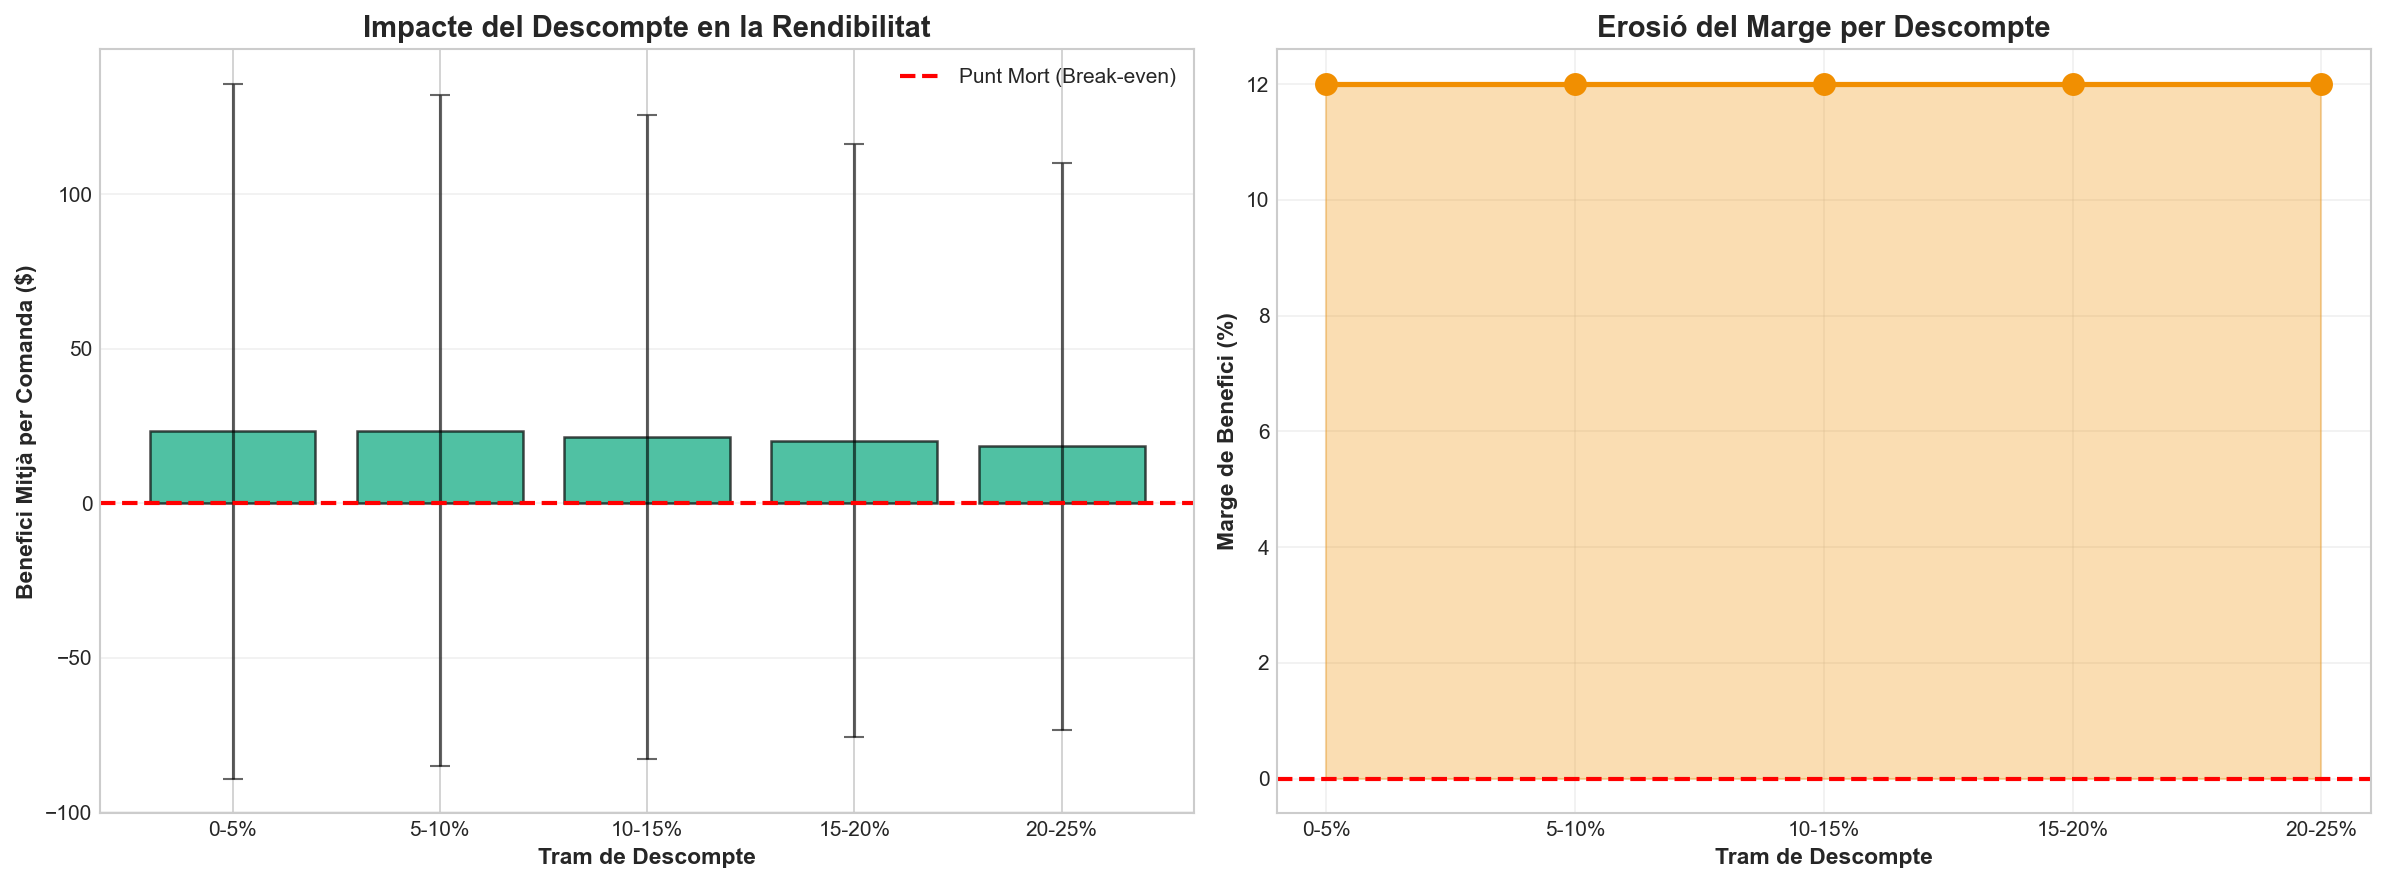
\includegraphics[width=1.0\textwidth]{figures/final/04_estudis_especifics/breakeven_analysis.png}
    \caption{Esquerra: Benefici en dòlars (barres verdes) per tram de descompte. Dreta: Marge de benefici en percentatge (línia taronja).}
    \label{fig:breakeven}
\end{figure}

Què estem veient exactament en aquest gràfic?
\begin{itemize}
    \item \textbf{La línia vermella (El perill):} La línia de punts vermella marca el zero (el punt on no guanyem ni perdem). Si les barres baixessin d'aquí, tindríem un problema greu.
    \item \textbf{La realitat (Barres Verdes):} Sorprenentment, \textbf{totes les barres estan per sobre de zero}. Fins i tot quan apliquem el descompte màxim possible (del 20 al 25\%), l'empresa segueix guanyant una mitjana de \textbf{18.41\$} nets per comanda.
    \item \textbf{L'enginyeria de preus (Línia Taronja):} Si mirem el gràfic de la dreta, veiem una línia taronja totalment plana. Això vol dir que el marge de benefici es manté estable al \textbf{12\%} independentment del descompte.
\end{itemize}

\textbf{Què vol dir això?} Que l'empresa té els preus molt ben calculats. Probablement, els productes amb molt descompte tenen un preu de sortida inflat artificialment per poder fer l'oferta després sense perdre diners realment.

\paragraph{2. La visió Macro: Què passaria si prohibim els descomptes?}
Ara que sabem que cada comanda individual és rendible, podríem pensar: ''D'acord, però si eliminem els descomptes, guanyarem MÉS diners, oi?''.

Per respondre a això, hem fet una simulació d'escenaris (Figura \ref{fig:scenario}). Hem calculat què passaria si demà l'empresa decidís prohibir tots els descomptes superiors al 12\%.

\begin{figure}[H]
    \centering
    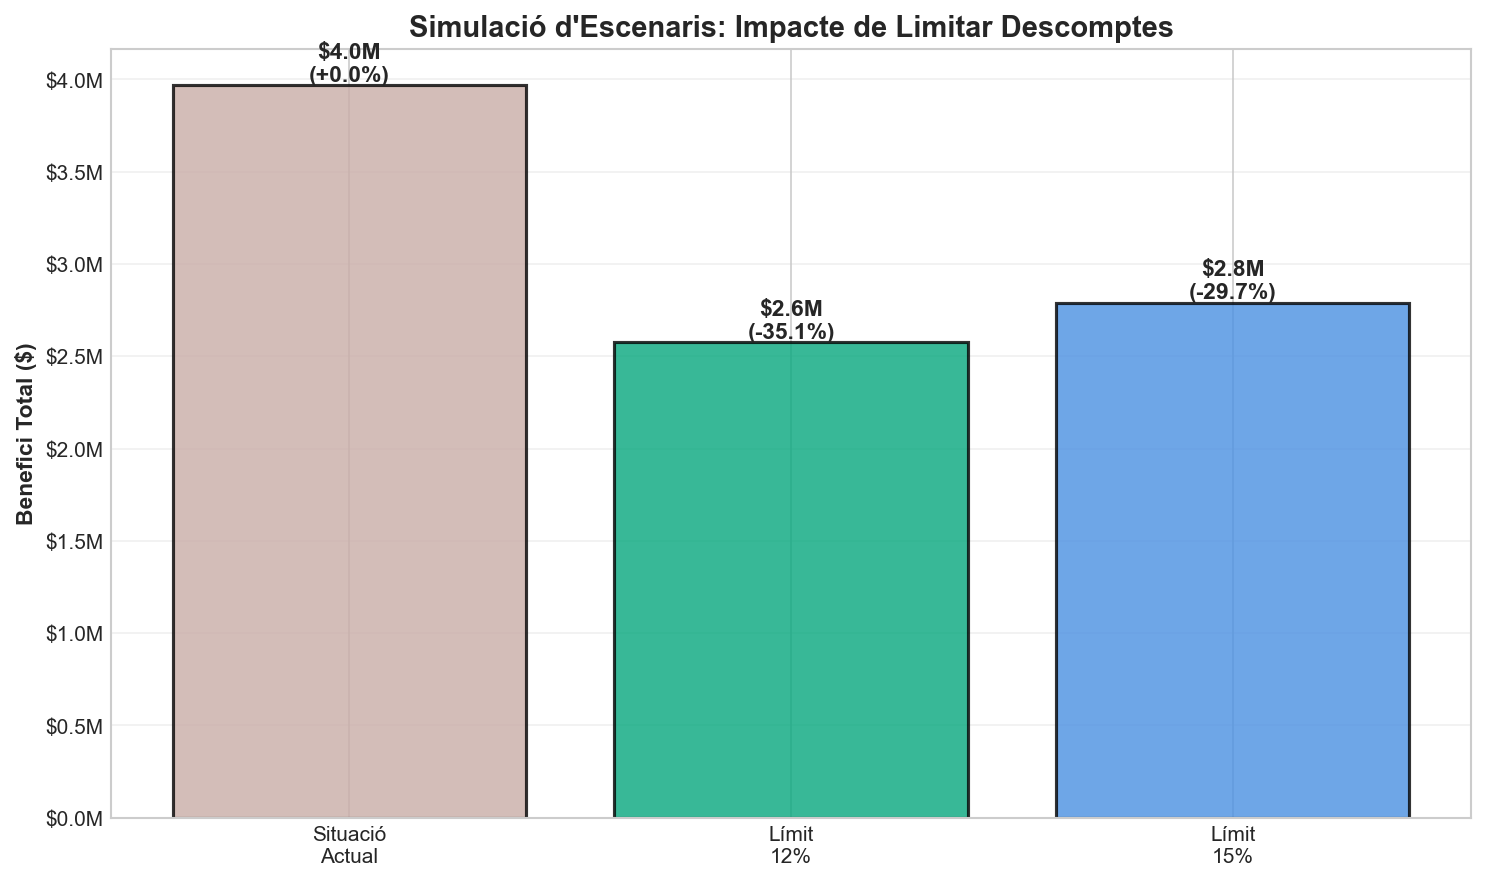
\includegraphics[width=0.8\textwidth]{figures/final/04_estudis_especifics/scenario_simulation.png}
    \caption{Simulació: La barra grisa és el benefici actual. La barra verda i blava és el benefici que tindríem si limitéssim els descomptes al 12 i 15\%.}
    \label{fig:scenario}
\end{figure}

El resultat de la simulació és molt clar:
\begin{itemize}
    \item \textbf{Pèrdua de Clients:} Si limitéssim els descomptes, molts clients deixarien de comprar perquè trobarien el producte car. Concretament, perdríem el volum de vendes de més de 70.000 comandes (un 39\% del total).
    \item \textbf{Impacte Econòmic:} La barres verda i blava són mes baixes que la grisa. Passaríem de guanyar 4 milions de dòlars a guanyar-ne només 2.6 milions. És a dir, perdríem 1.4 milions de dòlars de benefici (-35\%).
\end{itemize}

\paragraph{Conclusió Final de l'Estudi}
Les dades desmunten el mite. Els descomptes en aquesta empresa no són un problema, són una necessitat.
L'estratègia actual funciona així: acceptem guanyar una mica menys per cada unitat (baixant de 23\$ a 18\$) a canvi de vendre moltíssimes més unitats. Gràcies a aquest volum extra, el benefici total de l'empresa és molt més alt que si fóssim estrictes amb els preus.

\subsection{Resum de descobriments clau}
% Síntesi executiva dels insights més rellevants de la Part 1
Per tancar la fase d'anàlisi exploratòria i diagnòstic, sintetitzem la realitat operativa i financera de l'empresa en 12 punts crítics:

\begin{enumerate}
    \item \textbf{Crisi de Puntualitat:} El 54.8\% de les comandes arriben tard. La incapacitat de complir amb les dates d'entrega promeses és el punt més feble de l'operativa i afecta la majoria de clients.
    
    \item \textbf{La ''Estafa'' dels Enviaments Prèmium:} Existeix una correlació inversa entre preu i fiabilitat. Mentre que l'enviament estàndard és fiable, el servei \textit{First Class} té una taxa de fallada del \textbf{95.3\%}. El client paga més per un servei que sistemàticament arriba tard.
    
    \item \textbf{Invariància Geogràfica del Retard:} El patró de retards és idèntic a Europa, Àsia, Amèrica i Àfrica. Això descarta problemes de duanes locals i apunta a un \textbf{error de càlcul centralitzat} en la definició dels terminis d'entrega previstos.
    
    \item \textbf{Hiper-concentració de Vendes (Pareto 80/6):} La dependència del producte és extrema. Només 7 articles (el 5.9\% del catàleg) generen el 80\% de la facturació. L'empresa és vulnerable si falla qualsevol d'aquests ''Top Sellers''.
    
    \item \textbf{Risc de Proveïdor Únic:} Un sol producte (\textit{Field \& Stream Sportsman}) sosté el \textbf{18.8\%} de tots els ingressos globals (6.9M\$). Tota l'estabilitat financera penja d'un sol fil.
    
    \item \textbf{Evolució Negativa del Catàleg:} La salut de la cartera de productes ha empitjorat dràsticament el 2018, passant de necessitar 13 productes per fer el 80\% de les vendes a necessitar-ne només 4. La diversificació s'ha col·lapsat.
    
    \item \textbf{Robustesa del Marge (12\%):} Contràriament a la intuïció, els descomptes agressius no destrueixen la rendibilitat unitària. L'empresa manté un marge constant del 12\% fins i tot en els trams de descompte màxim, indicant una excel·lent enginyeria de preus.
    
    \item \textbf{El Perill de Limitar Descomptes:} La simulació demostra que prohibir els descomptes superiors al 12\% provocaria una \textbf{caiguda del 35\% en el benefici total} (-1.4M\$) degut a la pèrdua massiva de volum. Els descomptes són un motor necessari.
    
    \item \textbf{Clúster d'Oportunitat (Els que es refreden):} Mitjançant IA s'ha detectat un grup clau (29.4\% dels clients) que gasta molt (2.400\$) però que fa 9 mesos que no compra. Reactivar aquest grup és la prioritat nº1 de màrqueting.
    
    \item \textbf{Homogeneïtat del Client B2B/B2C:} No existeixen diferències de rendibilitat ni comportament entre clients particulars i corporatius. Les estratègies basades en tractar el client d'empresa com a VIP no tenen base financera en aquestes dades.
    
    \item \textbf{El Producte mana sobre el Mercat:} La rendibilitat depèn de \textit{què} es ven, no d'\textit{on} es ven. La categoria \textit{Fishing} és una mina d'or global, mentre que categories com \textit{Shop By Sport} tenen marges baixos a tots els continents.
    
    \item \textbf{Oportunitats de Nínxol:} Tot i la uniformitat global, s'han detectat anomalies positives, com l'èxit desproporcionat del \textit{Cardio Equipment} al mercat africà o la pesca als EUA, que permetrien estratègies regionals específiques.
\end{enumerate}

% ============================================================================
% 6. VISUALITZACIONS GEOGRÀFIQUES (PART 2)
% ============================================================================
\section{Visualitzacions geogràfiques interactives}

\subsection{Introducció a l'anàlisi geoespacial}
La cadena de subministrament que hem analitzat opera a escala global, connectant proveïdors i clients arreu del món. Per entendre aquesta dimensió espacial, hem complementat l'anàlisi estadística amb tècniques de visualització geogràfica.

Mitjançant la llibreria \texttt{Folium} de Python, hem creat 5 mapes interactius que s'exporten en format HTML. Aquests mapes permeten explorar les dades de manera dinàmica, amb funcions com el zoom, canvi de capes i finestres d'informació (\textit{popups}) que revelen detalls en passar el cursor o fer clic.

\subsection{Visualització 0: Panoràmica continental (La foto global)}

Abans d'entrar en el detall de països i ciutats, vam voler tenir una visió general de com es reparteix el negoci pel món. Aquest primer mapa ens dóna la ''foto gran'': quins continents venen més i quins donen més benefici.

\textbf{Per què aquest mapa?}
Quan tens dades de tot el món, és fàcil perdre's en els detalls. Aquest mapa respon a dues preguntes senzilles però importants:
\begin{itemize}
    \item \textbf{On es concentren les vendes?} Quins continents aporten més diners a la caixa?
    \item \textbf{On es guanya més per cada venda?} Quin és el marge real de benefici per continent?
\end{itemize}

\textbf{Com es va fer?}
Vam agrupar totes les comandes per continent, utilitzant un fitxer amb les fronteres mundials (\texttt{continents.geojson}). Després, vam pintar cada continent segons el total de vendes (com més fosc el color, més vendes) i vam afegir finestres d'informació que es mostren en passar el cursor.

\begin{figure}[H]
    \centering
    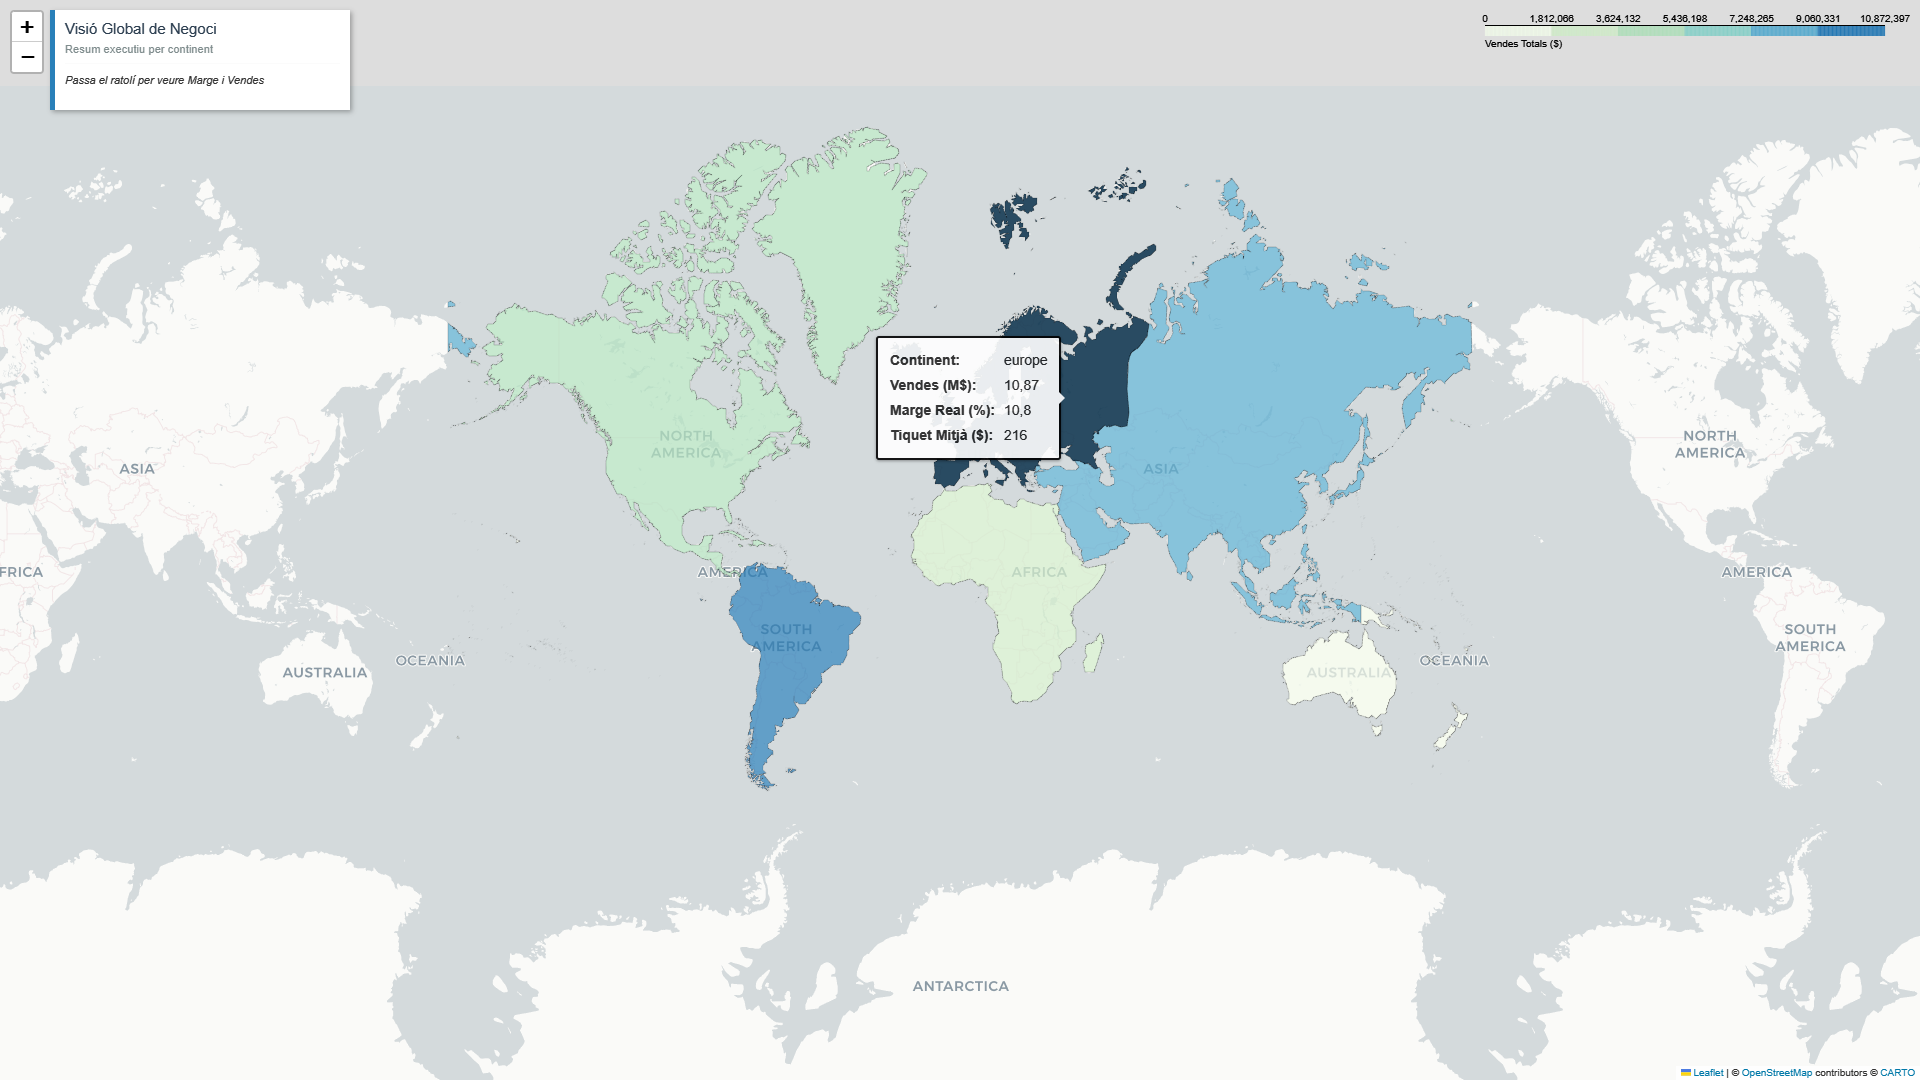
\includegraphics[width=1.0\textwidth]{figures/maps/map0.png} 
    \caption{Mapa 0: Visió general per continents. En passar el cursor sobre una regió es veuen les seves xifres clau.}
    \label{fig:map0}
\end{figure}

\textbf{Què ens va ensenyar?}
El mapa revela una geografia comercial amb dos grans pols i tres mercats secundaris:

\begin{itemize}
    \item \textbf{Els dos grans: Europa i Sudamèrica} dominen el negoci. Europa lidera en vendes (10,87M\$), seguida molt de prop per Sudamèrica (10,28M\$). Entre els dos sumen més del 60\% de la facturació global.
    
    \item \textbf{Sudamèrica: la sorpresa positiva} Tot i vendre lleugerament menys que Europa, Sudamèrica té un marge superior (10,9\% vs 10,8\%) i un tiquet mitjà sòlid (199\$). Això indica que és un mercat sòlid i rendible.
    
    \item \textbf{Nord-amèrica: el mercat rendible} Amb només 5,07M\$ de vendes, té el marge més alt de tots (11,1\%). Cada venda és més valuosa aquí, però el volum total és baix.
    
    \item \textbf{Àsia-Pacífic: el gegant amb rendibilitat ajustada} És el tercer mercat en vendes (8,27M\$) però amb el marge més baix (10,4\%). Venda molt, però amb marges comprimits.
    
    \item \textbf{Àfrica: el mercat emergent} Amb 2,29M\$, és el més petit, però té un marge saludable (11\%) i potencial de creixement.
\end{itemize}

\textbf{Conclusió pràctica:} El negoci es concentra a Europa i Sudamèrica, que són mercats madurs amb volums similars. La diferència estratègica és clara:

\begin{itemize}
    \item \textbf{A Europa (líder volum):} L'objectiu hauria de ser mantenir el lideratge però millorar la rendibilitat, potser revisant costos operatius o el mix de productes.
    
    \item \textbf{A Sudamèrica (sòlid i rendible):} Es pot aprofitar el bon marge per intentar créixer i superar Europa en vendes, ja que cada nova venda és rendible.
    
    \item \textbf{A Nord-amèrica (alta rendibilitat):} És el mercat on més es guanya per venda. Valdria la pena explorar per què no ven més.
\end{itemize}

Aquesta visió global ens diu que no cal anar a buscar nous continents: el potencial està a \textbf{Amèrica} (nord i sud), que combinada supera Europa en rendibilitat i té espai per créixer.
\subsection{Visualització 1: Risc de retard per país (Mapa de colors)}

Després de detectar una taxa global de retards del 55\%, la pregunta lògica era: \textit{És un problema concentrat en regions conflictives o és un problema mundial?} Aquest mapa de coropletes respon visualment a aquesta incògnita.

\textbf{Per què aquest mapa?}
L'objectiu era simple però crític: identificar si hi havia països o regions específiques on els retards fossin especialment greus. Si fos així, podríem actuar localment; si no, significaria que el problema és sistèmic i requereix una solució global.

\textbf{Com es va fer?}
Hem fusionat les dades de comandes amb la geometria de \texttt{countries.geojson}. Per a cada país, vam calcular el percentatge de comandes que arriben tard. Vam aplicar una escala de color lineal de tres nivells:
\begin{itemize}
    \item \textbf{Verd:} Baix risc de retard (menys del 40\%)
    \item \textbf{Taronja:} Risc mitjà (40\%-70\%)
    \item \textbf{Vermell:} Alt risc de retard (més del 70\%)
\end{itemize}

Els països sense dades apareixen en gris clar, ja que no tenim comandes o no hem pogut fer coincidir el nom amb el mapa.

\begin{figure}[H]
    \centering
    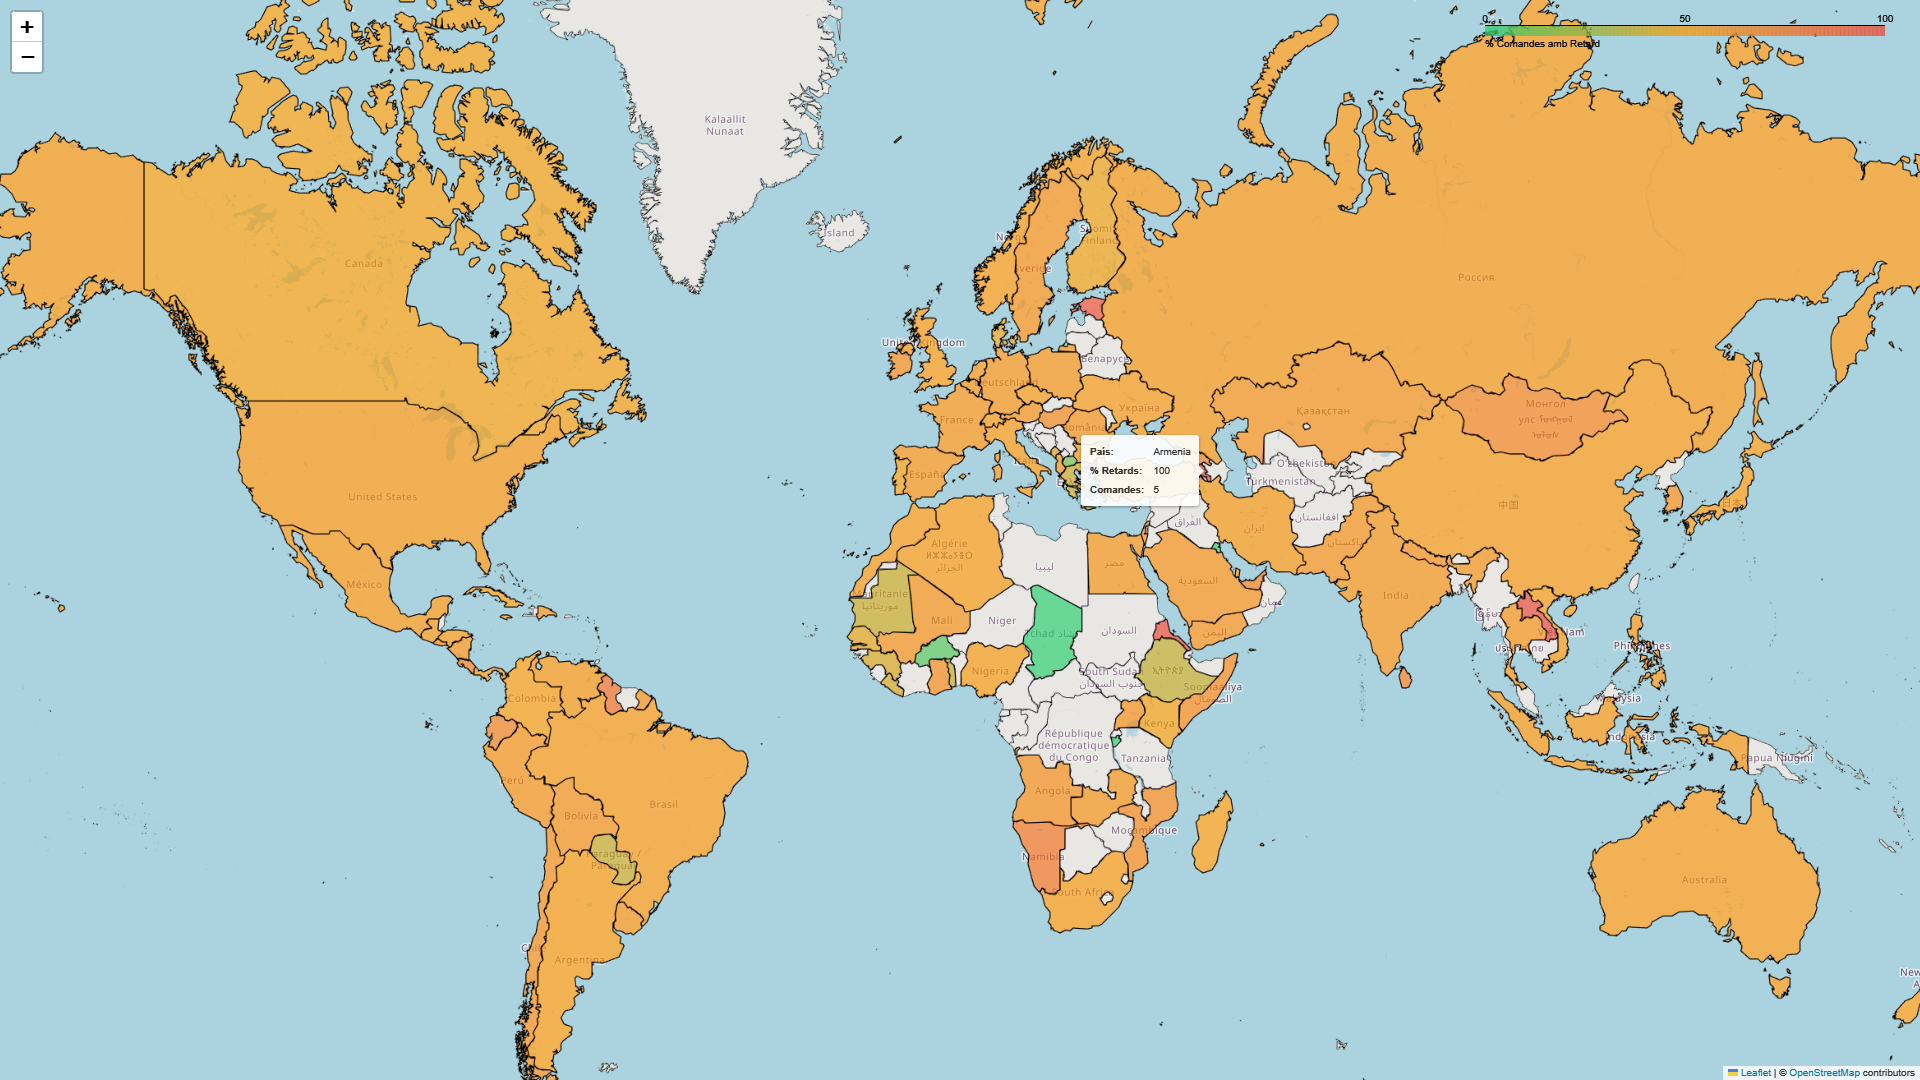
\includegraphics[width=1.0\textwidth]{figures/maps/map1.png} 
    \caption{Visualització 1: La ''Marea Taronja''. El mapa mostra una homogeneïtat preocupant en els retards a nivell global. El popup destaca el cas extrem d'Armènia (100\% retards).}
    \label{fig:map1}
\end{figure}

\textbf{Què ens va ensenyar?}
El resultat és revelador precisament per la seva \textbf{manca de contrast}. En lloc de veure zones vermelles i zones verdes clarament diferenciades, observem una \textbf{uniformitat taronja} a gairebé tots els mercats principals:

\begin{itemize}
    \item \textbf{El patró global (50-60\%):} Tant els Estats Units, com Europa Occidental, Brasil, la Xina i Austràlia comparteixen exactament la mateixa tonalitat. Això confirma visualment la hipòtesi de la ''Invariància Geogràfica'': no importa si el país és ric o en vies de desenvolupament, el sistema logístic falla en la meitat dels casos a tot arreu.
    
    \item \textbf{Mercats clau amb el mateix problema:}
    \begin{itemize}
        \item \textbf{Estats Units:} 55\% de retards
        \item \textbf{Alemanya:} 56\% de retards  
        \item \textbf{França:} 56\% de retards
        \item \textbf{Brasil:} 54\% de retards
        \item \textbf{Mèxic:} 55\% de retards
    \end{itemize}
    
    \item \textbf{Outliers (Casos Extrems):} Els únics punts que s'allunyen del taronja són països amb molt poques comandes on l'estadística es dispara.
    \begin{itemize}
        \item Com mostra el \textit{popup} de la captura, \textbf{Armènia} apareix en vermell intens amb un \textbf{100\% de retards} (5 comandes, totes tard).
        \item Alguns països africans com \textbf{Burkina Faso} apareixen en verd (9\% de retards), però probablement es deu a un volum de mostres insignificant (11 comandes) més que a una eficiència real.
    \end{itemize}
    
\end{itemize}

\textbf{Conclusió pràctica:} Aquest mapa canvia completament la perspectiva del problema:

\begin{enumerate}
    \item \textbf{No és un problema local:} No podem culpar a duanes específiques, proveïdors regionals o infraestructures locals. El problema és centralitzat.
    
    \item \textbf{La solució ha de ser global:} Cal revisar els processos centrals de l'empresa: càlcul de dates de lliurament promesa, selecció de transportistes globals, sistemes de seguiment.
    
    \item \textbf{Els outliers són enganyosos:} Països com Armènia (100\%) o Burkina Faso (9\%) no són representatius. L'atenció s'ha de centrar en els mercats principals que mostren el patró comú del 50-60\%.
\end{enumerate}

La ''Marea Taronja'' ens diu que estem davant d'una \textbf{fallida sistèmica}. L'empresa promet més del que pot complir a escala mundial, i aquest problema s'estén de manera uniforme per tot el planeta. No cal enviar equips a cada país; cal revisar el motor central de planificació logística.

\subsection{Visualització 2: Concentració i Rendibilitat (Mapa de Bombolles i Clusters)}

Si el mapa anterior ens donava una visió per països, aquest mapa de bombolles baixa al nivell de detall màxim: la ciutat. L'objectiu és identificar els nodes logístics reals i verificar si el volum de vendes es tradueix automàticament en beneficis.

\textbf{Repte Tècnic i Solució Interaactiva:}
Representar més de 11.000 ubicacions de venedors en un sol mapa presenta un problema de superposició visual (''overplotting''). Per resoldre-ho, hem implementat una visualització dual mitjançant \texttt{Folium Plugins}:
\begin{itemize}
    \item \textbf{Capa de Clusters (Agrupació):} Per a les vistes allunyades (zoom out), el mapa agrupa automàticament les ciutats properes en cercles verds amb un número (vegeu els clusters a Europa o Àsia a la Figura \ref{fig:map2}). Això permet quantificar la densitat de venedors per regió sense saturar la vista.
    \item \textbf{Capa Individual (Bombolles):} En fer zoom o desactivar l'agrupació, es revelen les bombolles individuals. Hem codificat dues variables visuals:
    \begin{itemize}
        \item \textbf{Mida (Radi):} Proporcional al volum de vendes (més gran = més facturació).
        \item \textbf{Color (Semàfor de Rendibilitat):} 
        Verd fosc ($>$40\$ benefici/comanda), 
        Verd clar (20-40\$), 
        Taronja (0-20\$) i 
        \textbf{Vermell (Pèrdues)}.
    \end{itemize}
\end{itemize}

\begin{figure}[H]
    \centering
    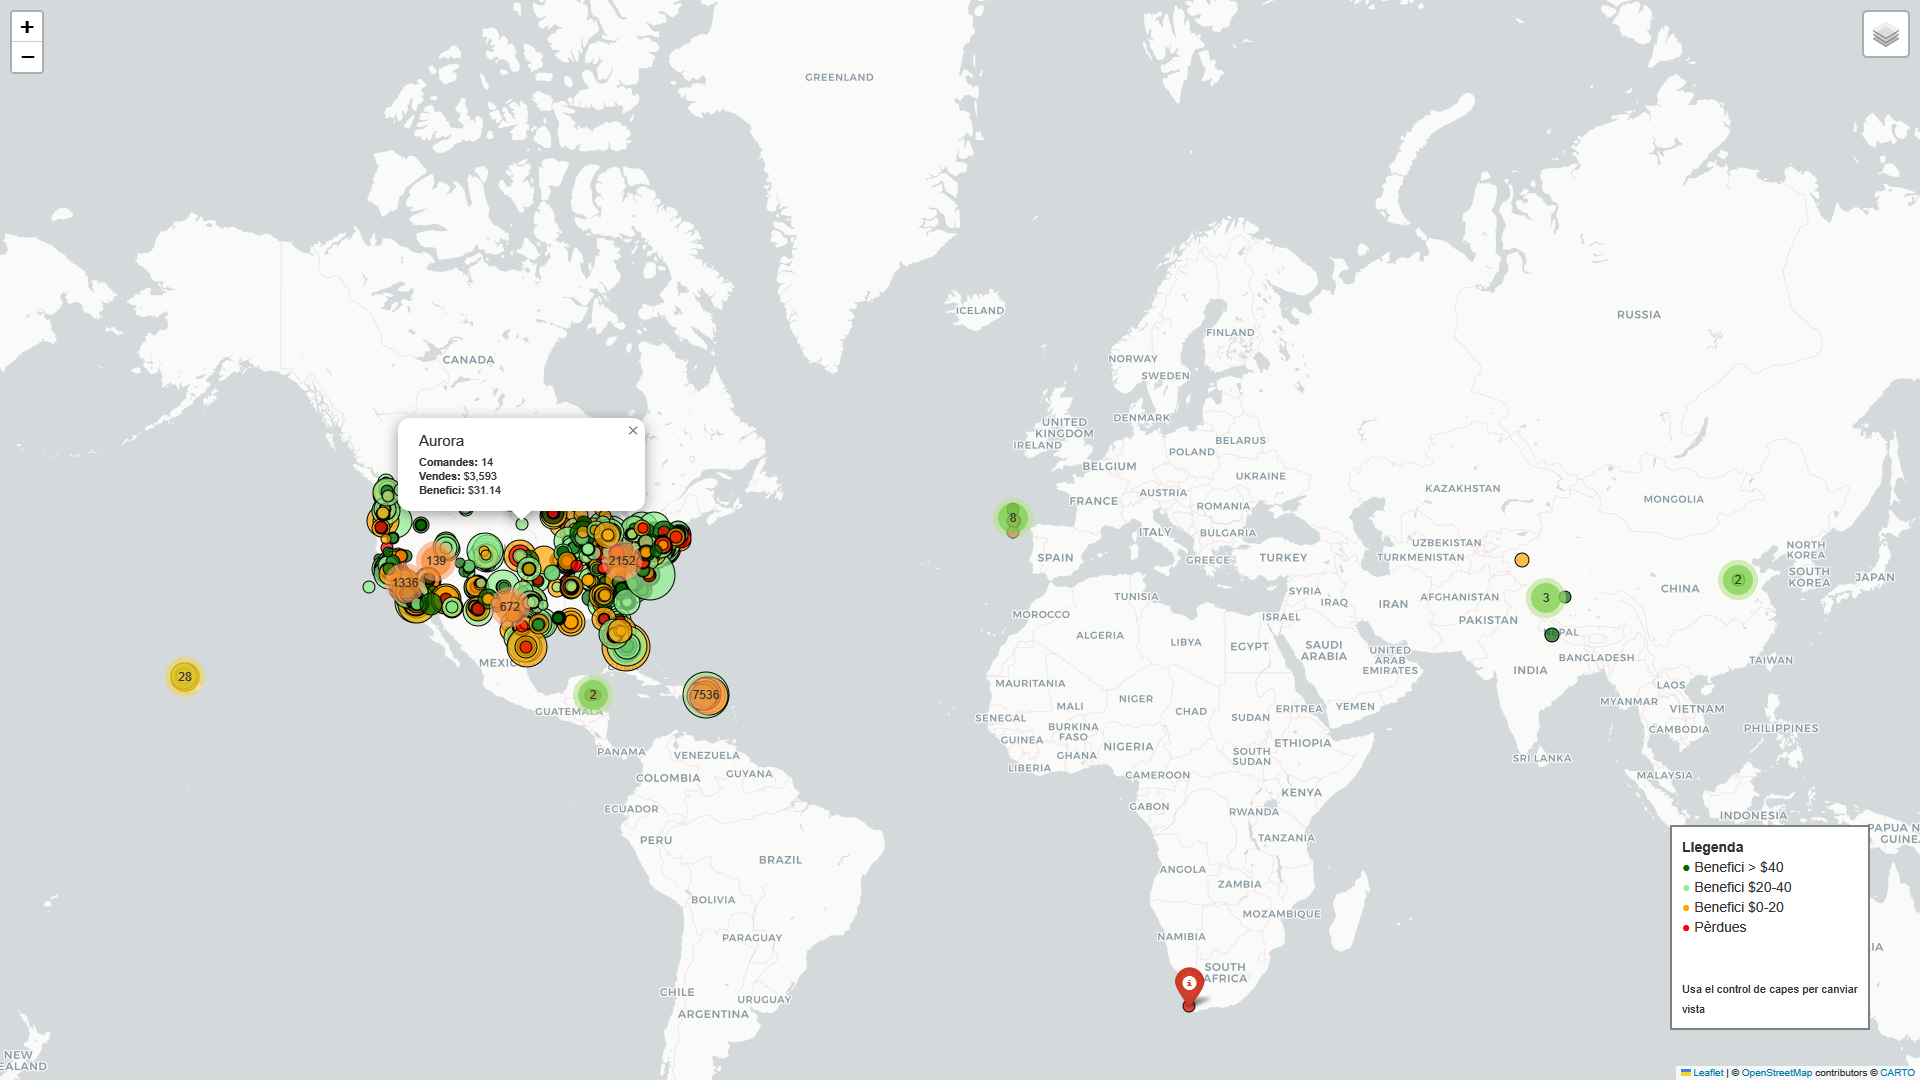
\includegraphics[width=1.0\textwidth]{figures/maps/map2.png} 
    \caption{Visualització 2: Mapa de Hubs Comercials. La captura mostra l'ús de popups per inspeccionar ciutats específiques (Ex: Aurora, EUA) i l'aparició d'alertes vermelles (Ex: Sud-àfrica).}
    \label{fig:map2}
\end{figure}

\textbf{Anàlisi de Casos (Lectura del Mapa):}
La interactivitat ens permet extreure conclusions immediates observant punts específics de la captura:
\begin{enumerate}
    \item \textbf{El cas d'Aurora (EUA):} El \textit{popup} desplegat ens mostra una ciutat mitjana-petita amb 14 comandes i 3.553\$ en vendes. Malgrat no ser un gran hub, el seu benefici és positiu (color verd/taronja). Aquest tipus de ciutats formen la ''Cua Llarga'' (\textit{Long Tail}) del negoci: milers de petits punts que, sumats, aporten volum.
    
    \item \textbf{L'Alerta a Sud-àfrica:} A la part inferior del mapa, observem un marcador de color \textbf{vermell intens}. Això indica que l'operació en aquest punt específic (zona de Ciutat del Cap) està generant pèrdues sistemàtiques. El mapa actua aquí com un sistema d'alerta primerenca per detectar fugues de diners en regions perifèriques.
    
    \item \textbf{La Concentració Americana:} La densitat de cercles superposats als Estats Units i el Carib contrasta radicalment amb la dispersió a Europa (on veiem un cluster de 8 punts) o Àsia (clusters de 2 o 3 punts). El negoci és, fonamentalment, americà.
\end{enumerate}

\textbf{Descobriment Estructural: El Monopoli de Caguas}
Més enllà dels detalls visuals, l'anàlisi de les dades subjacents al mapa revela una realitat estructural preocupant: la dependència extrema d'una sola ciutat, Caguas (Puerto Rico).
\begin{itemize}
    \item Mentre que la majoria de ciutats (com Aurora) gestionen desenes o centenars de dòlars, Caguas gestiona milions.
    \item Aquesta concentració representa un \textbf{Single Point of Failure (Punt únic de fallada)}. Un desastre natural (huracà) o un canvi regulatori a Puerto Rico paralitzaria una part crítica de la cadena de subministrament.
\end{itemize}

\textbf{Implicació Estratègica:}
El mapa ensenya un negoci amb dues velocitats. D'una banda, un nucli massiu i concentrat al Carib/EUA que requereix protecció de riscos. De l'altra, una xarxa dispersa global (els punts a Europa, Àsia, Àfrica) que presenta oportunitats d'expansió però també riscos de rendibilitat (punts vermells) que cal monitorar individualment.
\subsection{Visualització 3: El pols de la demanda (Mapa de Calor Temporal)}

Si el Mapa 2 ens mostrava l'estàtica de l'oferta, aquest tercer mapa introdueix la dimensió crítica del \textbf{temps}. Gràcies a l'animació mensual (2015-2018) i l'anàlisi del ''Top 10'' mensual, hem descobert que la demanda no és estable: es comporta com una \textbf{onada migratòria}.

\begin{figure}[H]
    \centering
    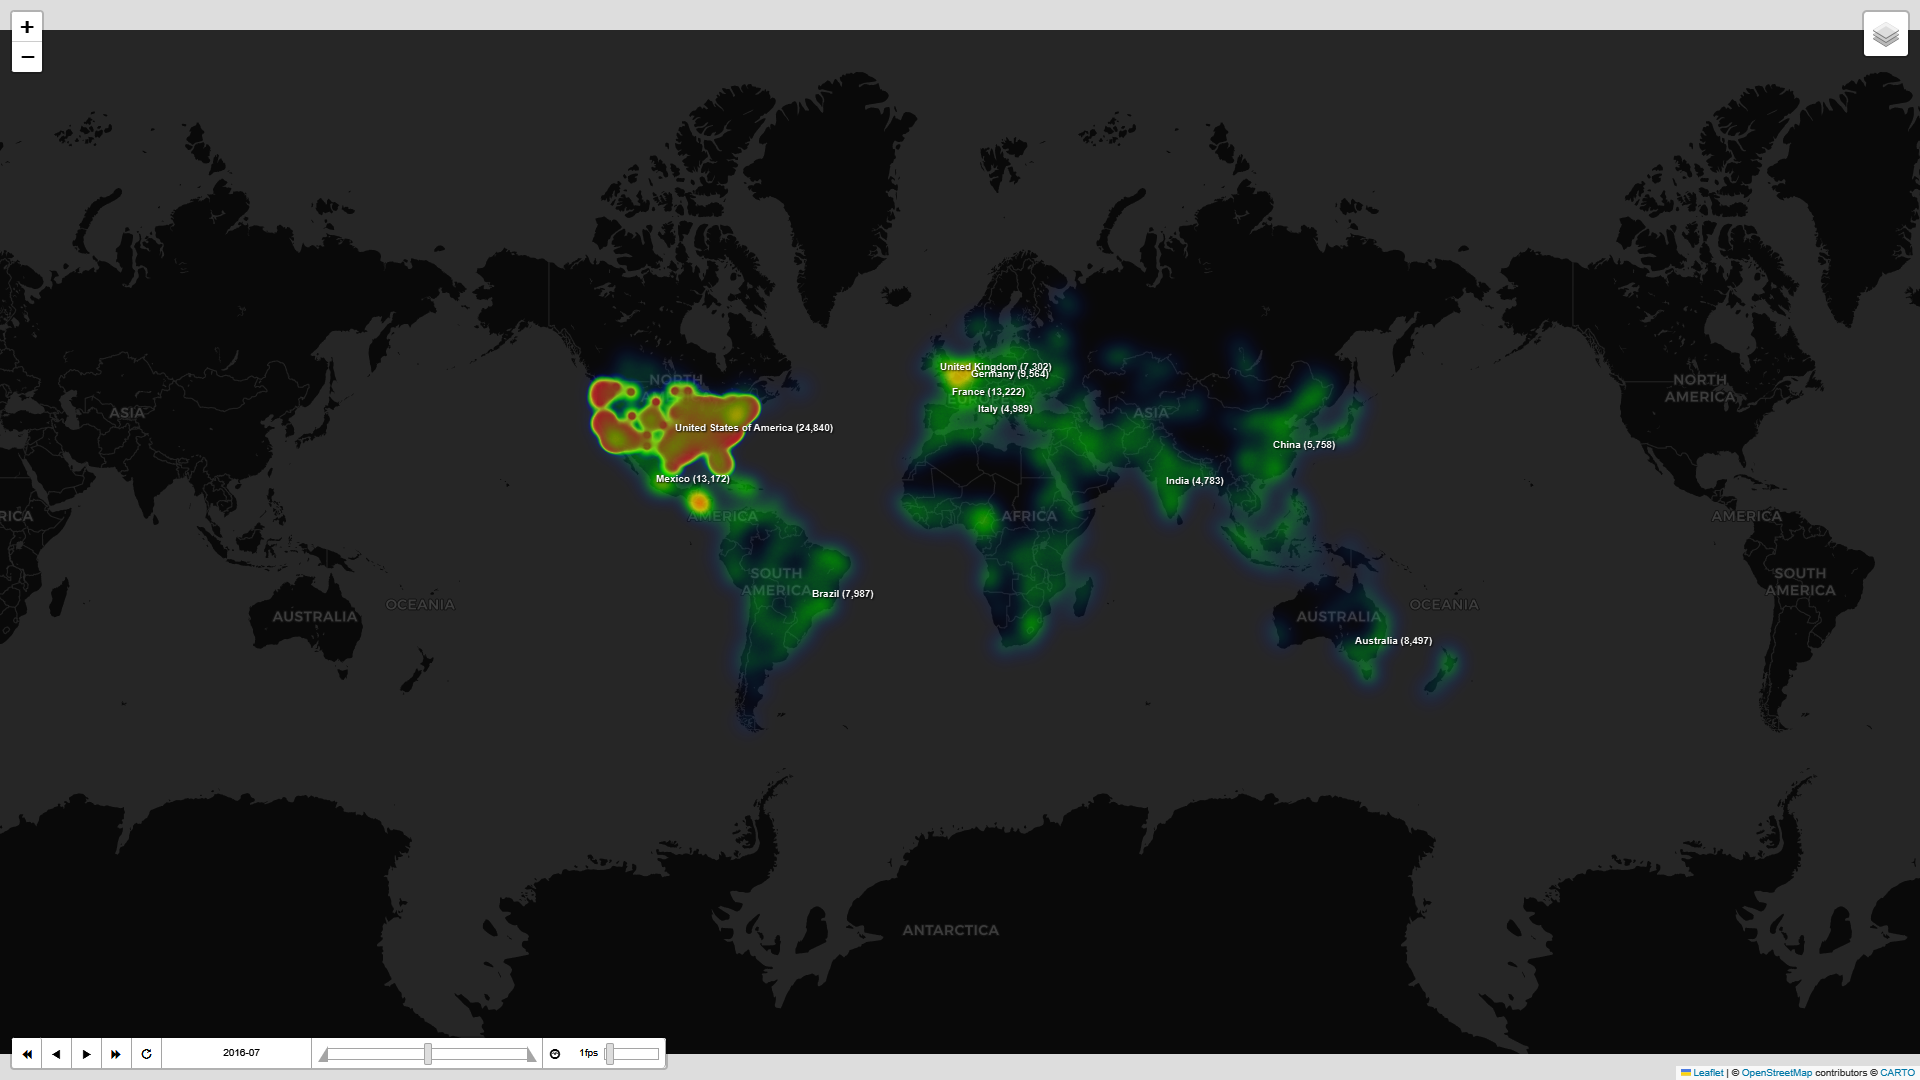
\includegraphics[width=1.0\textwidth]{figures/maps/map3.png} 
    \caption{Visualització 3: Mapa de Calor Temporal. La captura mostra la densitat de la demanda. L'animació del mapa revela com aquesta ''taca'' es desplaça geogràficament al llarg dels mesos.}
    \label{fig:map3}
\end{figure}

\textbf{Dinàmica Temporal: La teoria de la ''Demanda Nòmada''}
Contràriament a la creença inicial d'una expansió homogènia, les dades revelen que l'empresa focalitza els seus esforços comercials en regions específiques durant períodes concrets, creant cicles de mercat molt definits.

L'evolució segueix 4 fases estratègiques clares:

\begin{enumerate}
    \item \textbf{Fase 1: El Pèndol Atlàntic (2015 - 2016):}
    Durant els primers anys, la demanda oscil·la pendularment entre Amèrica Llatina i Europa:
    \begin{itemize}
        \item \textbf{Hivern/Primavera:} Domini absolut de LATAM. El gener de 2015, per exemple, el Top 5 és íntegrament llatinoamericà (Mèxic, Brasil, El Salvador, Rep. Dominicana, Cuba).
        \item \textbf{Estiu/Tardor:} El focus es desplaça a Europa. Al juny-setembre de 2015, França i Alemanya lideren el rànquing, desplaçant completament els països llatins.
    \end{itemize}

    \item \textbf{Fase 2: L'Anomalia dels Mercats Emergents (Finals 2016):}
    Entre agost i desembre de 2016, detectem un fenomen estrany. Els mercats tradicionals desapareixen i sorgeix un lideratge inesperat de països com \textbf{Turquia} (Líder amb ~700 comandes/mes), \textbf{Nigèria} i l'\textbf{Iran}. Això suggereix una campanya agressiva o una obertura temporal en mercats de l'Orient Mitjà i Àfrica (EMEA).

    \item \textbf{Fase 3: El Gegant Americà (Puntual):}
    Els Estats Units mostren un comportament explosiu però concentrat. Quan s'activen (ex: abril-juliol 2016), generen un volum massiu incomparable (\textbf{>5.000 comandes mensuals}, mentre que la resta de líders habituals ronden les 1.500). És un mercat de ''tot o res''.

    \item \textbf{Fase 4: El Gir Asiàtic Definitiu (Pivot to East - 2018):}
    La troballa més rellevant per al futur de l'empresa apareix als últims fotogrames de l'animació. A partir de novembre de 2017, Europa i LATAM s'enfonsen i Àsia pren el control absolut.
    \begin{itemize}
        \item \textbf{Gener 2018:} El canvi de paradigma es completa. El Top 5 mundial és, per primera vegada, 100\% de la regió Àsia-Pacífic:
        \begin{enumerate}
            \item \textbf{Austràlia} (543 comandes)
            \item \textbf{Índia} (375 comandes)
            \item \textbf{Xina} (361 comandes)
            \item \textbf{Indonèsia} (286 comandes)
            \item \textbf{Filipines} (123 comandes)
        \end{enumerate}
    \end{itemize}
\end{enumerate}

\textbf{Conclusió Operativa:}
L'empresa no té una demanda global estable, sinó que ''viatja''.
Això representa un repte logístic majúscul: no serveix de res tenir grans magatzems fixes a Europa si durant 6 mesos la demanda es mou a LATAM o Àsia.
\textit{Recomanació:} Cal passar d'una estructura logística estàtica a una de \textbf{flexible i modular}, capaç de seguir aquesta ''demanda nòmada'' que el 2018 s'ha instal·lat definitivament a l'Orient.
\subsection{Visualització 4: Fluxos Logístics (Flow Map)}

Fins ara hem vist punts estàtics al mapa (on venem i on comprem). Però la cadena de subministrament és moviment. Amb aquesta quarta visualització, connectem l'origen i el destí per revelar les artèries principals per on circulen els ingressos de la companyia.

\textbf{Disseny Tècnic: Dibuixant les connexions}
Hem filtrat el dataset per extreure les \textbf{Top 50 rutes comercials} per volum de facturació. Utilitzant la classe \texttt{PolyLine} de Folium, hem dibuixat línies que connecten la ciutat del venedor (\textit{Customer City}) amb la del comprador (\textit{Order City}).
El disseny incorpora dues variables visuals per facilitar la lectura ràpida:
\begin{itemize}
    \item \textbf{Gruix de la línia (Weight):} Proporcional a les vendes. Les rutes més gruixudes transporten més valor econòmic.
    \item \textbf{Codi de Colors (Rendibilitat):}
    \begin{itemize}
        \item \textbf{Verd:} Rutes molt rendibles (Benefici $>$ 20\$).
        \item \textbf{Taronja:} Rutes de marge ajustat (0-20\$).
        \item \textbf{Vermell:} Rutes deficitàries.
    \end{itemize}
\end{itemize}

\begin{figure}[H]
    \centering
    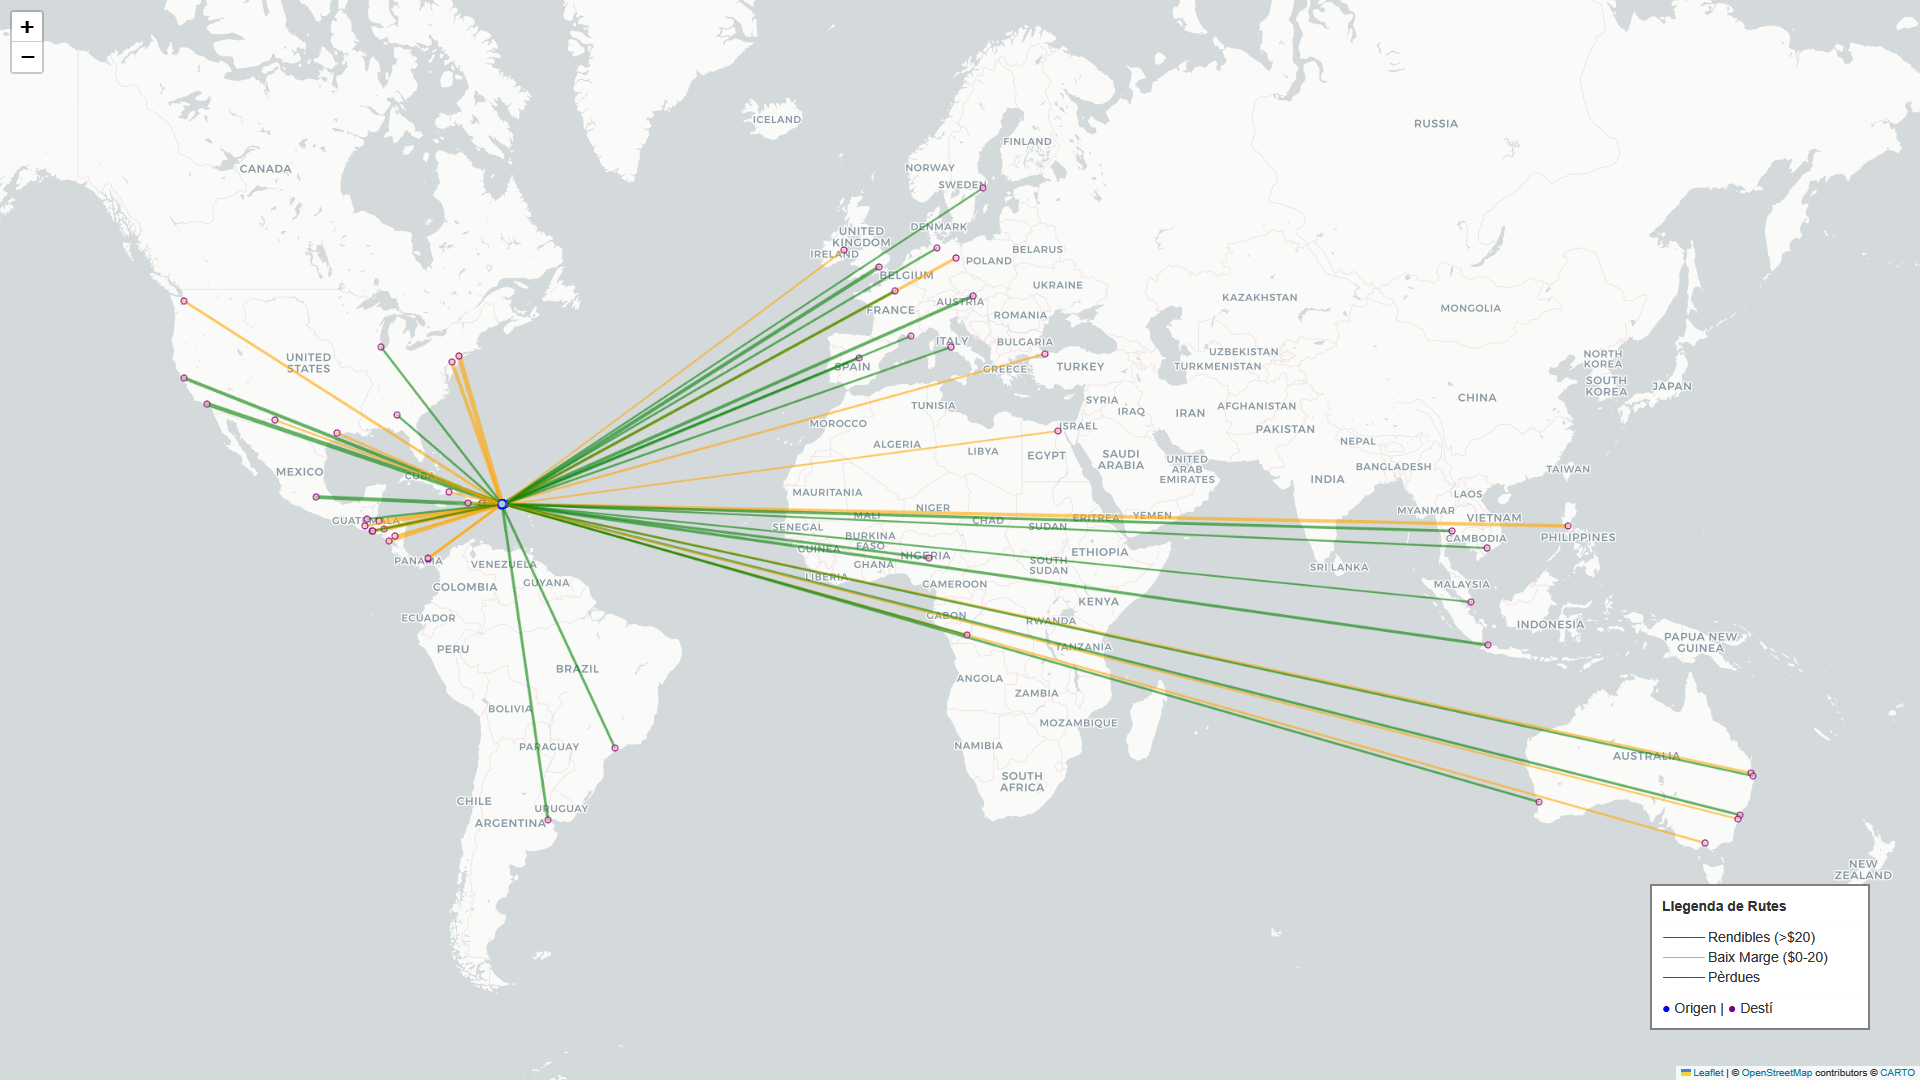
\includegraphics[width=1.0\textwidth]{figures/maps/map4.png} 
    \caption{Visualització 4: Mapa de Fluxos de les Top 50 rutes. S'observa una estructura radial perfecta amb centre a Puerto Rico.}
    \label{fig:map4}
\end{figure}

\textbf{Anàlisi de la Topologia: L'Efecte ''Aranya''}
El resultat visual és impactant per la seva simplicitat estructural. No veiem una malla complexa de connexions entre múltiples punts; veiem una \textbf{topologia radial (Hub-and-Spoke)} perfecta.

Analitzant les dades del Top 50 , confirmem el monopoli absolut d'un sol origen:
\begin{itemize}
    \item \textbf{L'Origen Únic:} Totes i cadascuna de les 50 rutes principals parteixen de \textbf{Caguas (Puerto Rico)}. Això converteix aquesta ciutat en el ''cor'' que bombeja sang a tot el sistema.
    \item \textbf{La Ruta Reina (Caguas $\rightarrow$ NYC):} La línia més gruixuda del mapa connecta Puerto Rico amb la ciutat de Nova York. Aquesta sola ruta genera \textbf{160.893\$} en vendes. Curiosament, està pintada de \textbf{taronja} (benefici mitjà 18.9\$), indicant que és una ruta de volum, no de marge.
    \item \textbf{Diversitat de Destins:} Des del centre a Caguas, les línies es disparen cap a:
    \begin{itemize}
        \item \textbf{Proximitat:} Santo Domingo (158.448\$, ruta taronja) i Tegucigalpa (134.007\$, ruta taronja).
        \item \textbf{Llarga Distància:} El mapa mostra línies que travessen l'oceà fins a destins sorprenents com \textbf{Manila} (Filipines) o \textbf{Perth} (Austràlia).
    \end{itemize}
\end{itemize}

\textbf{La Paradoxa de la Distància:}
Una troballa clau en observar els colors és que la distància no sembla penalitzar el benefici.
\begin{itemize}
    \item Les rutes curtes i massives (NYC, Santo Domingo) apareixen majoritàriament en \textbf{taronja} (marge baix).
    \item En canvi, rutes transoceàniques com \textbf{Caguas $\rightarrow$ Perth} o \textbf{Caguas $\rightarrow$ Estocolm} apareixen en \textbf{verd} (beneficis de 30\$ i 23\$ respectivament).
    \item Això suggereix que en els enviaments internacionals de llarga distància, l'empresa és capaç de repercutir millor els costos o ven productes de gamma més alta, protegint millor el marge que en les rutes domèstiques massives.
\end{itemize}

\textbf{Conclusió Operativa:}
El mapa de fluxos confirma una \textbf{vulnerabilitat crítica}: la centralització total. Tota la facturació surt del mateix port/aeroport a Puerto Rico. Un bloqueig logístic en aquest punt (vagues, huracans) tallaria immediatament les 50 artèries principals d'ingressos de la companyia.
\subsection{Visualització 5: Preferències Regionals (Mapa de Categories)}

Finalment, tanquem l'anàlisi geoespacial baixant al nivell del producte. La pregunta de negoci era: \textit{Hem d'adaptar el catàleg a cada cultura o tenim un producte global?} Aquest mapa analitza el ''Mix de Productes'' de cada regió per trobar la resposta.

\textbf{Disseny Tècnic: Agregació i Detall}
Per construir aquest mapa, hem processat centenars de línies de comandes per agrupar-les en 23 regions comercials.
\begin{itemize}
    \item \textbf{Mida del node (Importància):} Hem representat cada regió amb un cercle blau. El radi del cercle és proporcional al volum total de comandes (ex: el cercle d'Europa Occidental és molt més gran que el d'Àsia Central).
    \item \textbf{Informació al detall (Popups):} Com que no podem pintar 50 colors en un mapa sense crear caos, hem optat per una solució interactiva. En fer clic a cada regió, es desplega una taula amb el \textbf{Top 5 de Categories} més venudes i el seu pes percentual (vegeu Figura \ref{fig:map5}).
\end{itemize}

\begin{figure}[H]
    \centering
    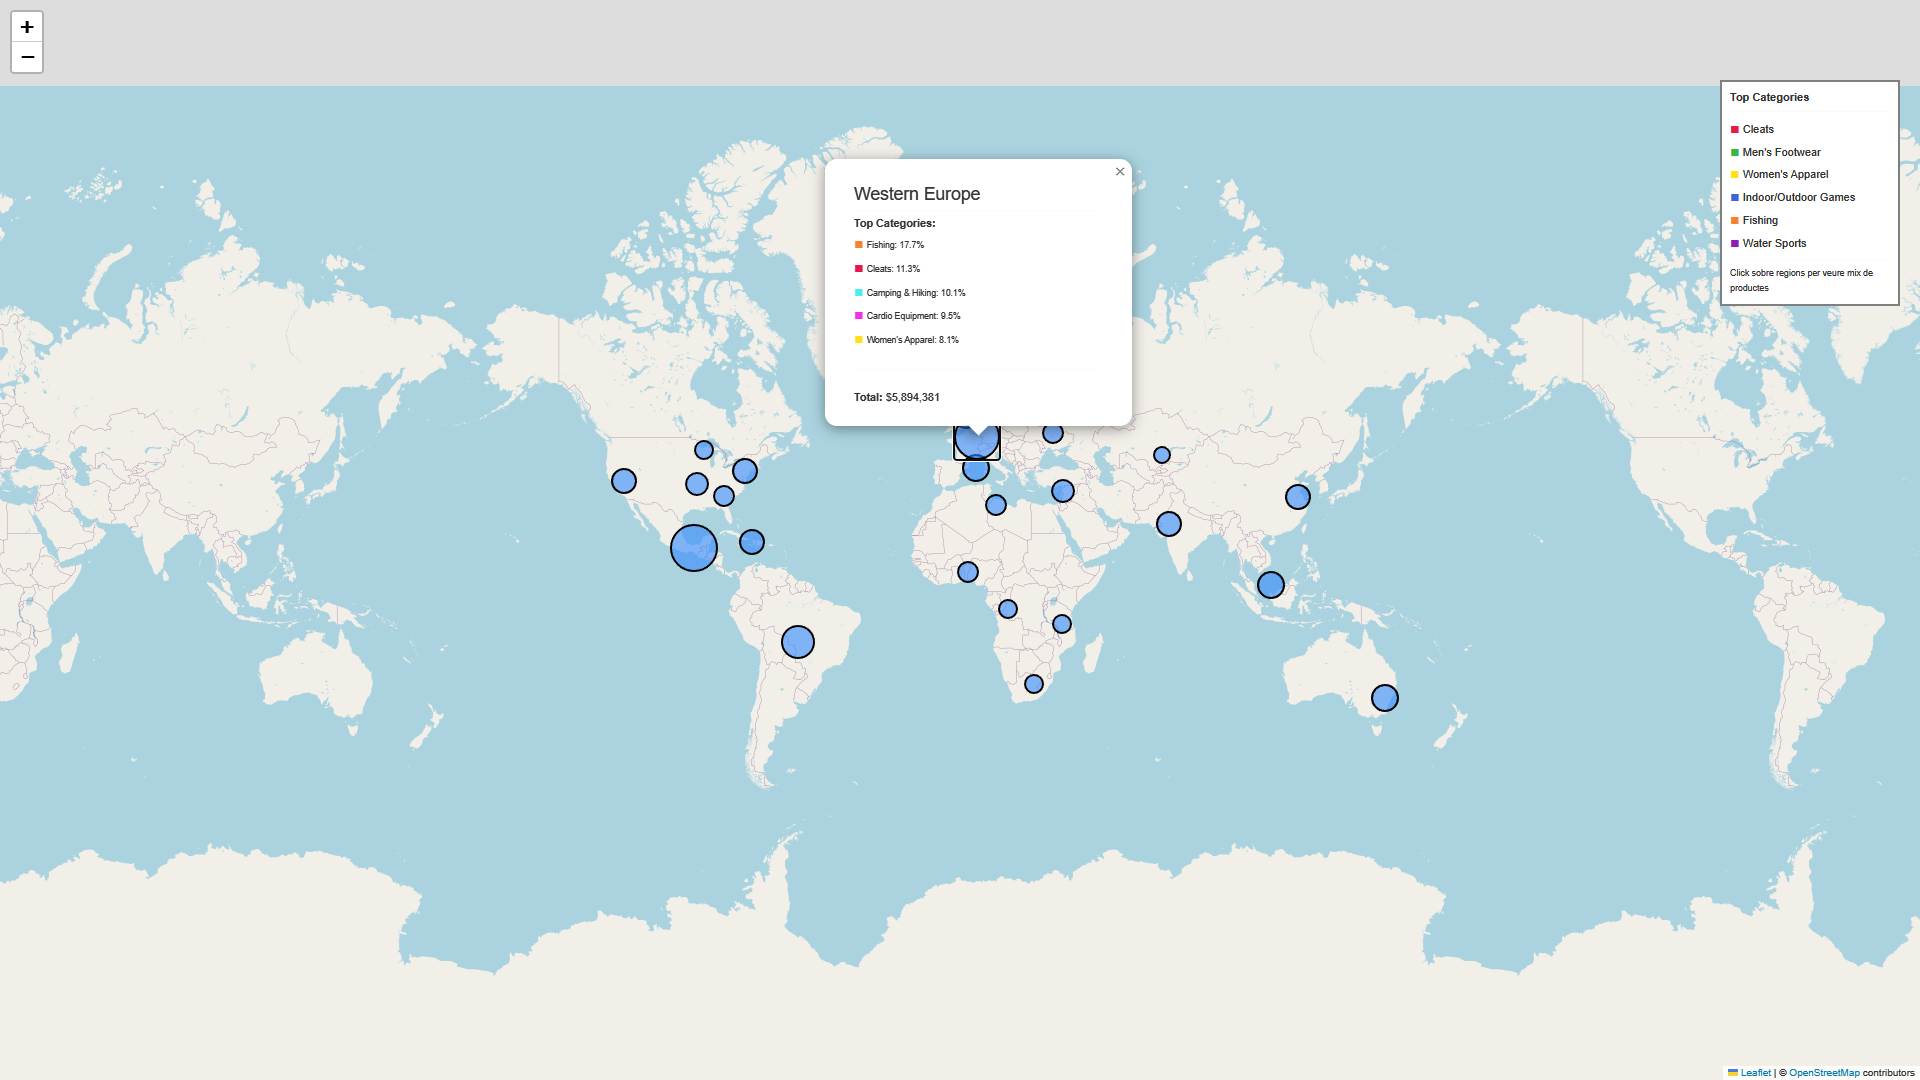
\includegraphics[width=1.0\textwidth]{figures/maps/map5.png} 
    \caption{Visualització 5: Preferències per Regió. El popup mostra el mix de productes d'una zona específica, revelant quines categories dominen el mercat local.}
    \label{fig:map5}
\end{figure}

\textbf{Anàlisi del Mix de Producte: La Uniformitat Global}
L'anàlisi de les dades subjacents revela una troballa contraintuïtiva: no hi ha diferències culturals significatives en el consum. El ''Top Seller'' és el mateix a la neu del Canadà que al desert de l'Oest Asiàtic.

Analitzem dos exemples extrems extrets de les dades:

\begin{itemize}
    \item \textbf{Canadà (Clima Fred / Nord-amèrica):}
    \begin{enumerate}
        \item \textbf{Fishing:} 14.8\% de les vendes.
        \item \textbf{Cleats (Botes de tac):} 13.7\%.
        \item \textbf{Cardio Equipment:} 13.2\%.
    \end{enumerate}
    
    \item \textbf{Oest Asiàtic (Clima Àrid / Orient Mitjà):}
    \begin{enumerate}
        \item \textbf{Fishing:} \textbf{20.2\%} de les vendes (Lideratge encara més fort).
        \item \textbf{Cleats:} 13.6\% (Idèntic al Canadà).
        \item \textbf{Camping \& Hiking:} 11.9\%.
    \end{enumerate}
\end{itemize}

\textbf{Patró Universal:}
Aquesta repetició sistemàtica de les categories \textit{Fishing} i \textit{Cleats} a les primeres posicions de gairebé totes les regions (des d'Àfrica fins a Europa) indica que:
\begin{enumerate}
    \item \textbf{L'Esport és Universal:} El futbol (representat per \textit{Cleats}) i l'activitat a l'aire lliure (\textit{Fishing}, \textit{Camping}) són transversals a totes les cultures del nostre mercat.
    \item \textbf{No existeix el ''Producte Local'':} No hem trobat cap regió on una categoria minoritària es converteixi de sobte en líder. El catàleg funciona en bloc.
\end{enumerate}

\textbf{Conclusió Estratègica:}
La uniformitat de la demanda simplifica enormement l'estratègia d'inventari.
\textit{Decisió:} No cal crear catàlegs personalitzats per regió ni estratègies de màrqueting hiper-locals. L'empresa pot aplicar una estratègia de producte global estandarditzada, ja que el que triomfa a Toronto també triomfa a Riad. Això permet economies d'escala massives en la compra de material (especialment en Pesca i Futbol).
% ============================================================================
% 7. CONCLUSIONS I RECOMANACIONS
% ============================================================================
% ============================================================================
% 7. CONCLUSIONS I RECOMANACIONS
% ============================================================================
\section{Conclusions i recomanacions}

\subsection{Síntesi dels resultats}
Aquest estudi ha transformat un conjunt de dades massiu en un diagnòstic precís sobre la salut de la cadena de subministrament. L'anàlisi exploratòria, financera i geoespacial revela una empresa amb una arquitectura de \textbf{doble velocitat}: financerament robusta gràcies a una enginyeria de preus excel·lent, però operativament crítica a causa d'una centralització excessiva i una logística de lliurament fallida.

Els quatre pilars que defineixen la realitat de l'empresa són:

\begin{enumerate}
    \item \textbf{Fragilitat del Catàleg (Ràtio 80/6):} L'empresa ha empitjorat la seva salut estructural. Si el 2017 necessitava 13 productes per fer el 80\% de les vendes, el 2018 el sistema s'ha col·lapsat i depèn de només 4 referències. Aquesta ''hiper-concentració'' supera qualsevol estàndard de risc acceptable.
    
    \item \textbf{Invariància del Fracàs Logístic:} Amb un 54.8\% de retards globals, el problema no és regional ni de duanes. Els mapes demostren que el retard és idèntic a tot el món (la ''Marea Taronja''), assenyalant un error sistèmic en el càlcul de les dates promeses, agreujat per una taxa de fallada del 95\% en els serveis prèmium.
    
    \item \textbf{Enginyeria de Preus Sòlida:} Contra tot pronòstic, l'estratègia de descomptes agressius és un èxit matemàtic. L'empresa aconsegueix mantenir un marge constant del 12\% independentment del descompte aplicat, utilitzant les ofertes com a motor de volum sense destruir valor.
    
    \item \textbf{Topologia Radial i Demanda Nòmada:} L'anàlisi geoespacial ha descobert que tota l'empresa penja d'un sol fil: el hub de Caguas (Puerto Rico). Aquesta estructura centralitzada xoca frontalment amb una demanda que és ''nòmada'' i que el 2018 s'ha desplaçat massivament cap a l'Àsia-Pacífic.
\end{enumerate}

\subsection{Resposta a les hipòtesis plantejades}
L'anàlisi rigorosa de les dades ha permès refutar la majoria de les intuïcions inicials, demostrant el valor de l'analítica de dades davant la suposició gerencial:

\begin{itemize}
    \item \textbf{H1: Els descomptes alts generen pèrdues.} \\
    \textbf{REFUTADA.} El benefici unitari es manté positiu (\$18.41) fins i tot amb descomptes del 25\%. La simulació demostra que limitar els descomptes seria catastròfic: provocaria una caiguda del 35\% en el benefici total per pèrdua de quota de mercat.
    
    \item \textbf{H2: Pagar més per l'enviament garanteix puntualitat.} \\
    \textbf{REFUTADA (La ''Paradoxa Logística'').} Existeix una correlació inversa entre cost i qualitat. Els enviaments \textit{Standard Class} (gratuïts/barats) són els més fiables, mentre que el \textit{First Class} falla sistemàticament. El client està pagant un sobrecost per un servei pitjor.
    
    \item \textbf{H3: El comportament de compra varia segons la cultura local.} \\
    \textbf{REFUTADA (Uniformitat Global).} L'anàlisi de categories per regió demostra que no existeix el ''producte local''. Categories com \textit{Fishing} i \textit{Cleats} són líders de vendes tant al Canadà com a l'Orient Mitjà. El catàleg és universal.
    
    \item \textbf{H4: Els retards depenen de la infraestructura del país de destí.} \\
    \textbf{REFUTADA.} El mapa de risc logístic mostra una homogeneïtat de colors (taronja) entre països desenvolupats i emergents. El problema és intern (processos de l'empresa), no extern (infraestructura del país).
\end{itemize}

\subsection{Limitacions de l'estudi}
\begin{itemize}
    \item \textbf{Manca de costos de transport real:} Sabem que la ruta Caguas $\rightarrow$ Austràlia és rendible, però no tenim el cost real de l'enviament marítim/aeri per validar si el marge absorbeix totalment la logística inversa (devolucions).
    \item \textbf{Finestra temporal (El tall del 2018):} L'estudi detecta l'inici del ''Pivot to East'' (explosió de vendes a Àsia) just al final de la sèrie temporal. No tenim dades del 2019 per confirmar si aquesta tendència s'ha consolidat.
\end{itemize}

\subsection{Recomanacions Estratègiques (Pla d'Acció)}
Basant-nos en les evidències, proposem un full de ruta urgent:

\begin{enumerate}
    \item \textbf{Descentralització Logística (Adaptació a la Demanda Nòmada):}
    L'estructura actual (tot surt de Puerto Rico) és ineficient per a una demanda que s'ha mogut a l'Àsia. 
    \textit{Acció:} Establir un centre de distribució satèl·lit (3PL) al sud-est asiàtic (Vietnam o Filipines) per reduir temps i costos cap al nou mercat principal.
    
    \item \textbf{Auditoria del Servei ''First Class'':}
    La taxa de fallada del 95\% en enviaments urgents és un risc reputacional inacceptable.
    \textit{Acció:} Suspendre temporalment l'opció de pagament per enviament ràpid o recalcular els algoritmes de predicció de dates (afegint +2 dies de marge de seguretat) immediatament.
    
    \item \textbf{Estratègia de Clients (Targeting Quirúrgic):}
    L'algorisme de clustering ha identificat 6.000 clients (Cluster 3) que gasten molt però s'estan ''adormint''.
    \textit{Acció:} Llançar campanyes de reactivació específiques per a aquest grup, evitant gastar pressupost en el Clúster 2 (clients ja perduts).
    
    \item \textbf{Gestió de Riscos (Diversificació):}
    L'empresa està massa exposada a un sol producte (\textit{Field \& Stream}) i un sol origen (Caguas).
    \textit{Acció:} Prioritzar la promoció de productes de categories secundàries (com \textit{Cardio Equipment}) per suavitzar la corba de Pareto i reduir la dependència del ''Top Seller''.
\end{enumerate}

\subsection{Conclusió final}
L'empresa es troba en un punt d'inflexió. Té un motor financer sa (preus i producte funcionen globalment) però un xassís operatiu trencat (logística centralitzada i lenta). Si no soluciona el problema dels retards i acompanya el desplaçament de la demanda cap a l'Àsia, corre el risc de morir d'èxit: vendre més del que pot entregar.
% ============================================================================
% REFERÈNCIES
% ============================================================================
% ============================================================================
% BIBLIOGRAFIA
% ============================================================================
\section{Referències Bibliogràfiques}

Per a l'elaboració d'aquest estudi, s'han consultat fonts acadèmiques i documentació tècnica especialitzada, amb especial èmfasi en les tècniques d'Intel·ligència Artificial aplicades a la segmentació de clients (Part 2 de l'estudi).

\subsection*{Algoritmes de Machine Learning i Segmentació (Clustering)}

\begin{itemize}
    \item \textbf{Sobre la metodologia combinada RFM + K-Means:} \\
    Christy, A. J., Umamakeswari, A., Priyatharsini, L., \& Neyaa, A. (2021). RFM ranking – An effective approach to customer segmentation. \textit{Journal of King Saud University - Computer and Information Sciences}, 33(8), 1171-1181. \\
    \textit{Justificació:} Aquest article acadèmic valida l'ús de les variables Recència, Freqüència i Monetari com a base sòlida per alimentar algorismes de clustering en comerç electrònic.

    \item \textbf{Sobre l'algorisme K-Means:} \\
    Scikit-learn Developers. (2023). \textit{Clustering: K-Means}. Scikit-learn: Machine Learning in Python. Recuperat de: \url{https://scikit-learn.org/stable/modules/clustering.html#k-means} \\
    \textit{Justificació:} Documentació oficial de la llibreria utilitzada, necessària per definir els paràmetres tècnics de l'algorisme (inicialització de centroides i convergència).

    \item \textbf{Sobre la validació del model (Mètode del Colze):} \\
    Bholowalia, P., \& Kumar, A. (2014). EBK-Means: A Clustering Technique based on Elbow Method and K-Means. \textit{International Journal of Computer Applications}, 105(9), 17-24. \\
    \textit{Justificació:} Referència clau per justificar la decisió matemàtica de triar $K=4$ segments, basant-se en la reducció de la distorsió (inèrcia) intra-clúster.
\end{itemize}

\subsection*{Gestió de la Cadena de Subministrament i Visualització}

\begin{itemize}
    \item \textbf{Sobre l'Anàlisi de Pareto i Inventaris:} \\
    Reid, R. D., \& Sanders, N. R. (2019). \textit{Operations Management: An Integrated Approach} (7th ed.). Wiley. \\
    \textit{Justificació:} Marc teòric que sustenta l'anàlisi ABC i la regla 80/20 aplicada a la concentració de vendes per producte (estudi de ''Blockbusters'').

    \item \textbf{Sobre la Intel·ligència Geoespacial (Supply Chain Mapping):} \\
    Mogos, R. C., et al. (2018). Spatial Analysis for Supply Chain Management. \textit{Amfiteatru Economic}, 20(49), 689-704. \\
    \textit{Justificació:} Fonamenta l'ús de mapes de calor i fluxos logístics per detectar patrons d'ineficiència en la distribució global.
\end{itemize}


% ============================================================================
% APÈNDIXS
% ============================================================================
\appendix
\section{Diccionari de Dades}
\label{app:data_dictionary}

El dataset original utilitzat en aquest estudi (\texttt{DataCoSupplyChainDataset.csv}) conté informació transaccional detallada. A continuació es descriuen les variables més rellevants utilitzades per a l'anàlisi exploratòria i els models predictius.

\begin{table}[H]
\centering
\caption{Descripció de les variables principals del dataset}
\label{tab:data_dict}
\resizebox{\textwidth}{!}{%
\begin{tabular}{l|l|p{8cm}}
\hline
\textbf{Nom Variable} & \textbf{Tipus} & \textbf{Descripció} \\ \hline
\texttt{Type} & Categòrica & Tipus de transacció (DEBIT, TRANSFER, PAYMENT, CASH). \\ \hline
\texttt{Days for shipping (real)} & Numèrica & Dies reals que va trigar l'enviament. \\ \hline
\texttt{Days for shipment (scheduled)} & Numèrica & Dies promesos al client per a l'entrega. \\ \hline
\texttt{Benefit per order} & Numèrica & Benefici net de la comanda (Ingressos - Costos). Pot ser negatiu. \\ \hline
\texttt{Sales per customer} & Numèrica & Total facturat al client (inclou impostos i descomptes). \\ \hline
\texttt{Delivery Status} & Categòrica & Estat final de l'enviament (Late Delivery, Shipping on time, etc.). \\ \hline
\texttt{Late\_delivery\_risk} & Binària & 1 si l'enviament va arribar tard, 0 si va ser puntual. \\ \hline
\texttt{Category Name} & Categòrica & Categoria del producte (Fishing, Cleats, Cardio, etc.). \\ \hline
\texttt{Customer City/Country} & Categòrica & Ubicació geogràfica del client (Destí). \\ \hline
\texttt{Order Region} & Categòrica & Regió comercial de destí (ex: Western Europe, South East Asia). \\ \hline
\texttt{Order Item Discount Rate} & Numèrica & Percentatge de descompte aplicat (0.00 a 0.25). \\ \hline
\end{tabular}%
}
\end{table}

\section{Implementació Tècnica (Python)}
\label{app:technical_code}

Aquest estudi s'ha realitzat utilitzant el llenguatge de programació Python (v3.9). A continuació es detallen les llibreries utilitzades i els fragments de codi clau per a la segmentació i visualització.

\subsection{Stack Tecnològic}
S'han utilitzat les següents llibreries per al processament i anàlisi:
\begin{itemize}
    \item \textbf{Pandas \& NumPy:} Manipulació i neteja de dades tabulars.
    \item \textbf{Matplotlib \& Seaborn:} Visualització estadística estàtica.
    \item \textbf{Folium:} Generació de mapes interactius (basat en Leaflet.js).
    \item \textbf{Scikit-learn:} Algorismes de Machine Learning (K-Means, StandardScaler).
\end{itemize}

\subsection{Codi clau: Clustering de Clients (K-Means)}
Per a la segmentació RFM, s'ha implementat el següent flux de treball: normalització de dades i aplicació de l'algorisme K-Means.

\begin{verbatim}
# 1. Preparació de dades RFM
scaler = StandardScaler()
rfm_normalized = scaler.fit_transform(rfm_df[['Recency', 'Frequency', 'Monetary']])

# 2. Aplicació de K-Means (amb K=4 segons mètode del colze)
kmeans = KMeans(n_clusters=4, random_state=42, n_init=10)
rfm_df['Cluster'] = kmeans.fit_predict(rfm_normalized)

# 3. Interpretació dels resultats
print(rfm_df.groupby('Cluster').agg({
    'Recency': 'mean',
    'Frequency': 'mean',
    'Monetary': 'mean',
    'customer_id': 'count'
}))
\end{verbatim}

\subsection{Codi clau: Generació del Mapa de Fluxos}
Per visualitzar les rutes comercials (Flow Map), s'ha utilitzat la funció \texttt{PolyLine} de Folium iterant sobre les rutes agrupades.

\begin{verbatim}
# Iterar sobre les rutes principals per dibuixar línies
for idx, row in routes_agg.iterrows():
    # Assignar color segons rendibilitat (Verd = bo, Vermell = dolent)
    if row['benefit_per_order'] < 0:
        color = 'red'
    elif row['benefit_per_order'] < 20:
        color = 'orange'
    else:
        color = 'green'
    
    # Dibuixar la línia origen -> destí
    folium.PolyLine(
        locations=[[row['lat_src'], row['lon_src']], 
                   [row['lat_dest'], row['lon_dest']]],
        color=color,
        weight=2.5,
        opacity=0.7
    ).add_to(map_flow)
\end{verbatim}
\section{Glossari de Termes}
\label{app:glossary}

Definició dels conceptes tècnics i mètriques utilitzades en aquest informe.

\begin{description}[leftmargin=3cm, style=nextline]
    
    \item[AntPath]
    Tècnica de visualització en mapes de flux que utilitza línies animades discontínues (simulant formigues) per indicar la direcció i velocitat d'un moviment entre dos punts geogràfics.
    
    \item[Break-even Point (Punt Mort)]
    Nivell d'activitat o preu a partir del qual els ingressos igualen als costos. En el context d'aquest estudi, es refereix al percentatge de descompte màxim que es pot aplicar sense incórrer en pèrdues mitjanes per comanda.
    
    \item[Choropleth Map]
    Mapa temàtic on les àrees geogràfiques (països, regions) es tenyeixen de colors amb una intensitat proporcional al valor d'una variable estadística (ex: taxa de retard).
    
    \item[Clustering (K-Means)]
    Algorisme d'aprenentatge automàtic no supervisat que agrupa dades en ''k'' grups (clústers) basant-se en la seva similitud matemàtica, minimitzant la variància intra-grup.
    
    \item[EDA (Exploratory Data Analysis)]
    Fase inicial de l'anàlisi de dades que utilitza estadística descriptiva i visualització per descobrir patrons, detectar anomalies i comprovar hipòtesis.
    
    \item[Heatmap (Mapa de Calor)]
    Representació gràfica de dades on els valors individuals es representen com a colors. Utilitzat aquí per veure la densitat geogràfica de les comandes i la matriu de rendibilitat per categoria/mercat.
    
    \item[Kurtosis (Curtosi)]
    Mesura estadística que determina el grau de concentració que presenten els valors d'una variable al voltant de la zona central de la distribució de freqüències (puntxeguda vs plana).
    
    \item[Late Delivery Risk]
    Variable binària (0/1) que indica si una comanda té una probabilitat alta d'arribar més tard de la data promesa, basant-se en l'històric d'enviaments similars.
    
    \item[Outlier (Valor Atípic)]
    Observació que es desvia tant d'altres observacions que desperta sospites que va ser generada per un mecanisme diferent (ex: una venda de 100.000\$ en un dataset amb mitjana de 200\$).
    
    \item[Pareto Principle (80/20)]
    Regla empírica que suggereix que, per a molts esdeveniments, aproximadament el 80\% dels efectes provenen del 20\% de les causes. En el nostre cas, el 80\% de vendes provenen d'un nombre molt reduït de productes.
    
    \item[RFM (Recency, Frequency, Monetary)]
    Model de segmentació de màrqueting que avalua tres dimensions: fa quant temps va comprar el client (Recència), quantes vegades compra (Freqüència) i quant gasta (Valor Monetari).
    
    \item[Skewness (Asimetria)]
    Mesura de la manca de simetria d'una distribució de probabilitat. Una asimetria positiva indica una cua llarga a la dreta (molts valors baixos i pocs de molt alts).

\end{description}


% ============================================================================
% FI DEL DOCUMENT
% ============================================================================
\end{document}
